\def\catalan{0}
\def\coloring{0}
\documentclass[a4paper,UKenglish,cleveref,autoref]{lipics-v2019}

\hypersetup{
    colorlinks=true,
    linkcolor=Sepia,
    citecolor=ForestGreen,
    urlcolor=RoyalBlue}

\usepackage[dvipsnames]{xcolor}

\usepackage{algorithm}
\usepackage{thm-restate}
\usepackage{mathtools}
\usepackage[noend]{algpseudocode}
\usepackage[colorinlistoftodos]{todonotes}
\usepackage[T1]{fontenc}
\usepackage{relsize}
%\usepackage{multirow}
\usetikzlibrary{
  shapes.multipart,
  matrix,
  positioning,
  shapes.callouts,
  shapes.arrows,
  calc}


\def\bo{\mathcal{O}}
\def\Bo{\mathlarger{\mathcal{O}}}
\def\bt{\Theta}
\def\polylog{\mathrm{polylog}\;}

\DeclarePairedDelimiter\floor{\lfloor}{\rfloor}
\newcommand{\SL}[2]{\sum\limits_{#1}^{#2}}
\newcommand{\BSL}[2]{\mathlarger{\mathlarger{\sum}\limits_{#1}^{#2}}}
\newcommand{\PL}[2]{\prod\limits_{#1}^{#2}}
\newcommand{\BPL}[2]{\mathlarger{\mathlarger{\prod}\limits_{#1}^{#2}}}
\newcommand{\func}[1]{\texttt{\textsc{#1}}}
\newcommand{\distr}[1]{\mathsf{#1}}
\newcommand{\matr}[1]{\mathbf{#1}}
\newcommand{\data}[1]{\mathbf{#1}}
\def\poly{\mathrm{poly}}

\def\filled{\textup{\textsf{filled}}}
\def\unfilled{\textup{\textsf{unfilled}}}

\def\ZERO{\mathsf{0}}
\def\ONE{\mathsf{1}}
\def\PHI{\phi}
\def\LAST{\matr{last}}
\def\BUCKET{\matr{bucket}}
\def\BEGIN{\matr{begin}}
\def\END{\matr{end}}
\def\ADJ{\matr{A}}

\newcommand{\sectioninput}{\input}

\usepackage{bm}

\renewcommand{\vec}[1]{\mathbf{#1}}
\graphicspath{{./images/}}


\bibliographystyle{alpha}

\title{Miscellaneous Results}

\date{}
\author{Amartya Shankha Biswas}{CSAIL, MIT}{asbiswas@mit.edu}{https://orcid.org/0000-0002-5068-1524}{funding}
\author{Ronitt Rubinfeld}{CSAIL, MIT}{ronitt@csail.mit.edu}{}{funding}
\author{Anak Yodpinyanee}{CSAIL, MIT}{anak@csail.mit.edu}{https://orcid.org/0000-0002-7572-2003}{funding}

\authorrunning{A.\,S. Biswas}

\keywords{Dummy keyword}%TODO mandatory; please add comma-separated list of keywords

\nolinenumbers

\hideLIPIcs


\begin{document}

\maketitle

\begin{abstract}

\todo[inline,color=red!80!green!25]{Consistency, keywords and spell check}
\todo[inline]{Kleinberg}
Consider an algorithm performing a computation on a \emph{huge random object} (for example a random graph or a ``long'' random walk).
Is it necessary to generate the entire object prior to the computation,
or is it possible to provide query access to the object and sample it incrementally ``on-the-fly'' (as requested by the algorithm)?
Such an \emph{implementation} should emulate the random object by answering queries in a manner consistent with
an instance of the random object sampled from the true distribution (or close to it).
This paradigm is useful when the algorithm is sub-linear and thus, sampling the entire object up front would ruin its efficiency.

Our first set of results focus on undirected graphs with independent edge probabilities,
i.e. each edge is chosen as an independent Bernoulli random variable.
We provide a general implementation for this model under certain assumptions.
Then, we use this to obtain the first efficient local implementations for the Erd\"os-R\'enyi $G(n,p)$ model for \emph{all} values of $p$,
and the Stochastic Block model.
As in previous local-access implementations for random graphs, we support \func{Vertex-Pair} and \func{Next-Neighbor} queries.
In addition, we introduce a new \func{Random-Neighbor} query.
Next, we give the first local-access implementation for \func{All-Neighbors} queries in the (sparse and directed) Kleinberg's Small-World model.
Our implementations require no pre-processing time, and answer each query using $ \mathcal{O}(\poly(\log n)) $ time, random bits, and additional space.

Next, we show how to implement random Catalan objects, specifically focusing on Dyck paths
(balanced random walks on the integer line that are always positive).
Here, we support $\func{Height}$ queries to find the location of the walk,
and $\func{First-Return}$ queries to find the time when the walk returns to a specified location.
This in turn can be used to implement $\func{Next-Neighbor}$ queries on random rooted and binary trees,
and $\func{Matching-Bracket}$ queries on random well bracketed expressions (the Dyck language).

Finally, we define a new model that allows us to generate a richer class of random objects that do not have a succinct description.
Specifically, we study uniformly random \emph{valid} $q$-colorings of an input graph $G$ with maximum degree $\Delta$.
This is in contrast to prior work in the area, where random objects are defined as a distribution with $\mathcal O(1)$ parameters
(for example, $n$ and $p$ in the $G(n,p)$ model).
The distribution over valid colorings of $G$ is instead specified via a ``huge'' input (the underlying graph $G$),
that is far too large to be read by a sub-linear time algorithm.
Instead, our implementation accesses the description through local neighborhood probes to $G$.

This new model can be compared to \emph{Local Computation Algorithms}, which also implement query access to a consistent valid solution,
and read their input using local probes.
Inspired by this connection, we extend our model to support implementations that are memory-less.
This setting allows multiple independent (possibly simultaneous) instantiations to agree on the same random object, without any communication.
When $q > \alpha\Delta$ for a small constant $\alpha$, we show how to implement queries to the color of any given node in sub-linear time,
such that the resulting colors are consistent with a single valid coloring drawn from the uniform distribution.
Unlike LCAs which can return an arbitrary valid solution, our model requires a uniformly random one.

\end{abstract}

\newpage

\tableofcontents
\newpage

\section{Introduction}
Consider an algorithm performing a computation on a \emph{huge random object} (for example a random graph or a ``long'' random walk).
Is it necessary to generate the entire object prior to the computation,
or is it possible to provide query access to the object and sample it incrementally ``on-the-fly'' (as requested by the algorithm)?
Such an \emph{implementation} would emulate the random object by answering appropriate queries in a consistent manner.
Specifically, all responses to queries must be consistent with an instance of the random object sampled from the true distribution (or close to it).
This paradigm is useful when the algorithm is sub-linear and thus, sampling the entire object up front would ruin its efficiency.
The problem of sampling partial information about huge random objects was pioneered in \cite{huge_old,huge}.
Further work in \cite{sparse,reut} considers the generation of different random graph models.
\todo[inline,color=Red!20]{Add more citations}

\todo[inline,color=Red!20]{In this paper, we . . . Finish}
One emerging theme that we develop further in this work is to provide common data-structure query access to huge random objects.
For example, for random graph implementations, in addition to supporting adjacency matrix queries about the existence of edge $(u,v)$,
\cite{reut} introduced the study of $\func{Next-Neighbor}$ queries which provide efficient access to the adjacency list representation.

For example, the greedy routing algorithm on Kleinberg's small world networks \cite{kleinberg} only uses $\mathcal O(\log^2 n)$ probes.
Using our implementation, one can execute this algorithm on a random small world instance
in $\mathcal O(\poly(\log n))$ time without incurring the $\mathcal O(n)$ prior-sampling overhead.




\subsection{Random Graphs}%
\label{sec:random_graphs}
In Section~\ref{sec:undirected}, we implement queries to both the adjacency matrix and adjacency list representation
for the generic class of \emph{undirected graphs} with {\em independent edge probabilities} $\left\{ p_{uv} \right\}_{u,v\in V}$,
where $p_{uv}$ denotes the probability that there is an edge between $u$ and $v$.
We implement \func{Vertex-Pair}, \func{Next-Neighbor}, and \func{Random-Neighbor}
\footnote{\func{Vertex-Pair}$(u,v)$ returns whether $u$ and $v$ are adjacent, \func{Next-Neighbor}$(v)$ returns a new neighbor of $v$ each time
it is invoked (until none is left), and \func{Random-Neighbor}$(v)$ returns a uniform random neighbor of $v$ (if $v$ is not isolated).} queries.
Under reasonable assumptions on the ability to compute certain values pertaining to consecutive edge probabilities,
our implementations support all three types of queries using $\mathcal{O}(\poly(\log n))$ time, space, and random bits.
Note that in this setting, $\func{Vertex-Pair}$ queries are trivial, since the existence of an edge depends on an independent random variable.
As in \cite{reut} (and unlike many of the implementations presented in \cite{huge_old,huge}), our techniques allow unlimited queries.
In particular, our construction yields local-access implementations for the Erd\"{o}s-R\'{e}nyi $G(n,p)$ model (for \emph{all} values of $p$),
and the Stochastic Block model with random community assignment.
\begin{table}[htpb]
\centering
\renewcommand{\arraystretch}{1}
\begin{tabular}{| >{\centering\arraybackslash}m{120pt} || >{\centering\arraybackslash}m{50pt} | >{\centering\arraybackslash}m{60pt} | >{\centering\arraybackslash}m{70pt} | >{\centering\arraybackslash}m{60pt} |}
    \hline
    \textbf{Model}              & \func{Vertex-Pair} & \func{Next-Neighbor} & \func{Random-Neighbor} & \func{All-Neighbors} \\      \hline \hline
    $G(n,p)$ with $p=\frac{\log^{\mathcal O(1)} n}{n}$
                                & \cite{sparse}      & \cite{sparse}        & \cite{sparse}          & \cite{sparse}        \\[5pt] \cline{1-5}
    $G(n,p)$ for arbitrary $p$  & This paper         & This paper           & This paper             & \UBD                 \\[5pt] \cline{1-5}
    Stochastic Block Model with $\log^{\mathcal O(1)} n$ communities
                                & This paper         & This paper           & This paper             & \UBD                 \\[5pt] \cline{1-5}
    BA Preferential Attachment  & \cite{reut}        & \cite{reut}          & \BD                    & \UBD                 \\[5pt] \cline{1-5}
    Small world model           & This paper         & This paper           & This paper             & This paper           \\[5pt] \cline{1-5}
    Random ordered rooted trees & This paper         & This paper           & This paper             & This paper           \\[5pt] \cline{1-5}
    \end{tabular}
    \vspace{0.7em}
    \caption{\textbf{(Local access implementations for random graphs):}
        All the implementations in this table use polylogarithimc time, additional space and random bits per query.
        A \UBD\ in the \func{All-Neighbors} column indicates that the graphs in this model may have un-bounded degree,
        and it is therefore impossible to sample \func{All-Neighbors} efficiently.
        A \BD\ entry indicates a sampling problem with no known efficient solution.}
    \label{table:graph_results}
\end{table}


While \func{Vertex-Pair} and \func{Next-Neighbor} queries, as well as \func{All-Neighbors} queries for sparse graphs,
have been considered in the prior works of \cite{reut, huge_old, huge, sparse},
we provide the first implementations of non-sparse random graph models.
Prior results for implementing queries to $G(n,p)$ focused on the sparse case where $p = \log^{\mathcal O(1)} n/n$ \cite{sparse}.
The dense case where $p = \Theta(1)$ is also relatively simple because most of the adjacency matrix is filled,
and neighbor queries can be answered by performing $\Theta(1)$ \func{Vertex-Pair} queries until an edge is found.
The interesting case is when $p$ takes on some intermediate value; say $p = 1/\sqrt{n}$.
In this regime, each vertex has high degree $\mathcal O(\sqrt{n})$ but most of the adjacency matrix is empty,
thus making it difficult to sample a neighbor efficiently.
We also provide the first implementation (to the best of our knowledge) of \func{Random-Neighbor} queries in \emph{non-sparse graphs}.
Such queries are useful, for instance, in sub-linear algorithms that employ random walk processes.


\paragraph*{Directed Random Graphs: The Small World Model}
\label{par:directed_random_graphs}
We then consider local-access implementations for directed graphs in Kleinberg's Small World model,
where the probabilities are based on distances in a 2-dimensional grid.
Building on our previous sampling procedure, we implement \func{All-Neighbors} queries for the Small World model,
using $\mathcal{O}(\poly(\log n))$ time, space and random bits (since such graphs are sparse, the other queries follow directly).




\subsection{Catalan Objects}%
\label{sec:intro_catalan_objects}
We show how to provide query access to very long ($2n$ step) one dimensional random walks,
One obvious query of interest is $\func{Height}(t)$ which returns the position of the walk at time $t$.
We also introduce and support \func{First-Return} queries, where $\func{First-Return}(t)$ returns
the first time when the random walk returns to the same level as it was at time $t$.
\func{Height} queries for the simple unconstrained random walk
follow trivially from the implementation of interval summable functions presented in \cite{huge}.
Here, we focus on an important generalization by considering balanced random walks (equal number of up and down steps) on the integer line,
that are constrained to be always positive (commonly known as Dyck Paths).
The added constraint introduces intricate non-local dependencies on the distribution of positions.
However, we are able to support both queries using $\mathcal O(\poly(\log n))$ resources.

Dyck paths are one type of Catalan object, and they have natural bijections to other Catalan objects
such as bracketed expressions, random rooted trees and binary trees.
Thus, we can use our Dyck Path implementation to obtain useful implementations of other random Catalan objects.
For instance, $\func{Height}$ queries correspond to $\func{Depth}$ queries on rooted trees and bracketed expressions
(Section~\ref{sec:bijections_to_other_catalan_objects}).
We also support more involved queries that are widely used; for example, finding the children of a node in a random tree
or finding the matching bracket in a random bracketed expression.
To achieve this, we note that \func{First-Return} queries queries correspond to $\func{Next-Neighbor}$ queries on trees,
and $\func{Matching-Bracket}$ queries on bracketed expressions (Section~\ref{sec:bijections_to_other_catalan_objects}).




\subsection{Random Coloring of Graphs}%
\label{sec:random_coloring_of_graphs}
Finally, we introduce a new model for implementating huge random objects with \emph{huge input description};
that is, the distribution is specified as a uniformly random solution to a huge combinatorial problem.
In this model, we implement query access to random $q$-colorings of a given huge graph $G$ with maximum degree $\Delta$.
A random coloring is sampled by proposing $\mathcal O(n\log n)$ color updates and accepting the ones that do not create a conflict (Glauber dynamics).
This is an inherently sequential process with the acceptance of a particular proposal depending on all preceding neighboring proposals.
Moreover, unlike the previously considered random objects, this one has no succinct representation, and we can only uncover the proper distribution
by probing the graph (in the manner of \emph{local computation algorithms} \cite{LCA, LCA_space_efficient}).
Unlike LCAs which have to return \emph{some} valid solution, we also have to make sure that we return a solution from the correct distribution.
We are able to construct an efficient oracle that returns the final color of a vertex using only a sub-linear number of probes when $q\ge 7\Delta$.




\subsection{Related Work}
\label{sec:related_work}
The problem of computing local information of huge random objects was pioneered in \cite{huge_old,huge}.
Further work of \cite{sparse} considers the generation of sparse random $G(n,p)$ graphs from the Erd\"{o}s-R\'{e}nyi model \cite{er},
with $p = O(\poly(\log n)/n)$, which answers $\poly(\log n)$ \func{All-Neighbors} queries, listing the neighbors of queried vertices.
While these implementations use polylogarithmic resources over their entire execution,
they generate graphs that are  only guaranteed to \emph{appear random} to algorithms that inspect a \emph{limited portion} of the generated graph.

In \cite{reut}, the authors construct an oracle for the generation of recursive trees, and BA preferential attachment graphs.
Unlike prior work, their implementation allows for an arbitrary number of queries.
This result is particularly interesting --  although the graphs in this model are generated via a sequential process,
the oracle is able to locally generate arbitrary portions of it and answer queries in polylogarithmic time.
Though preferential attachment graphs are sparse, they contain vertices of high degree,
thus \cite{reut} provides access to the adjacency list through \func{Next-Neighbor} queries.

For additional related work, see Section~\ref{sec:related_work}.

\section{Preliminaries}
\label{sec:model}
\subsection{Local-Access Generators}
\label{sec:oracle_model}

We begin by formalizing a model of {\em local-access generators} (Section~\ref{sec:oracle_model}), implicitly used in \cite{reut}.
\todo{Not good}
Our work provides local-access generators for various basic classes of graphs described in the following, with 
\func{Vertex-Pair}, \func{Next-Neighbor}, and \func{Random-Neighbor} queries.
In all of our results, each query is processed using $\poly(\log n)$ time, random bits, and additional space, with \emph{no initialization overhead}.
These guarantees hold even in the case of adversarial queries.
Our bounds assume constant computation time for each arithmetic operation with $O(\log n)$-bit precision.
Each of our generators constructs a random graph drawn from a distribution that is $1/\poly(n)$-close to the desired distribution in the $L_1$-distance.
\footnote{The \emph{$L_1$-distance} between two probability distributions $\distr{p}$ and $\distr{q}$ over domain $D$
is defined as $\|\distr{p-q}\|_1 = \sum_{x \in D } |p(x)-q(x)|$.
We say that $\distr{p}$ and $\distr{q}$ are $\epsilon$-close if $\|\distr{p-q}\|_1 \leq \epsilon$.}

We consider the problem of locally generating random graphs $G = (V,E)$ drawn from the desired families of simple unweighted graphs, undirected or directed. We denote the number of vertices $n = |V|$, and refer to each vertex simply via its unique ID from $[n]$. For undirected $G$, the set of neighbors of $v \in V$ is defined as $\Gamma(v) = \{u \in V: \{v,u\} \in E\}$; denote its degree by $\deg(v) = |\Gamma(v)|$.
Inspired by the goals and results of \cite{reut}, we define a model of local-access generators as follows.
\begin{definition}
A \emph{local-access generator} of a random graph $G$ sampled from a distribution $\distr{D}$,
is a data structure that provides access to $G$ by answering various types of
\emph{supported queries}, while satisfying the following:
%For clarity, we assume that the generator is invoked until its entire graph $G$ is exposed.
%The local-access generator for a probability distribution $\distr{D}$ of the desired random graph model must satisfy the following properties:
\begin{itemize}
\item \textbf{Consistency.} The responses of the local-access generator to all probes throughout the entire execution must be consistent with a single graph $G$.
\item \textbf{Distribution equivalence.} 
The random graph $G$ provided by the generator must be sampled from some distribution $\distr{D}'$
that is $\epsilon$-close to the desired distribution $\distr{D}$ in the $L_1$-distance.
In this work we focus on supporting $\epsilon = n^{-c}$ for any desired constant $c>0$.
As for \func{Random-Neighbor}$(v)$, the distribution from which a neighbor is returned
must be $\epsilon$-close to the uniform distribution over neighbors of $v$
with respect to the sampled random graph $G$ (w.h.p $1-n^{-c}$ for each query).
\item \textbf{Performance.} The resources, consisting of (1) computation time, (2) additional random bits required, and (3) additional space required, in order to compute an answer to a single query and update the data structure, must be sub-linear, preferably $\poly(\log n)$.
\end{itemize}
\end{definition}
In particular, we allow queries to be made adversarially and non-deterministically. The adversary has full knowledge of the generator's behavior and its past random bits.

For ease of presentation, we allow generators to create graphs with self-loops.
When self-loops are not desired, it is sufficient to add a wrapper function that simply re-invokes \func{Next-Neighbor}$(v)$ or \func{Random-Neighbor}$(v)$ when the generator returns $v$.


\paragraph*{Supported Queries in our Model} 
For undirected graphs, we consider queries of the following forms.
now we might want to do \func{Next-Neighbor} first for consistency.
\begin{itemize}
\item \func{Next-Neighbor}$(v)$: The generator returns the neighbor of $v$ with the lowest ID that has not been returned during the execution of the generator so far. If all neighbors of $u$ have already been returned, the generator returns $n+1$.
\item \func{Random-Neighbor}$(v)$: The generator returns a neighbor of $v$ uniformly at random (with probability $1/\deg(v)$ each). If $v$ is isolated, $\bot$ is returned.
\item \func{Vertex-Pair}$(u,v)$: The generator returns either $\ONE$ or $\ZERO$, indicating whether $\{u,v\}\in E$ or not.
\item \func{All-Neighbors}$(v)$: The generator returns the entire list of out-neighbors of $v$. We may use this query for relatively sparse graphs, specifically in the Small-World model.
\end{itemize}

\subsection{Random Graph Models}
\label{sec:graph_model}

\paragraph*{Erd\"{o}s-R\'{e}nyi Model}
We consider the $G(n, p)$ model: each edge $\{u,v\}$ exists independently with probability $p \in [0, 1]$.
Note that $p$ is not assumed to be constant, but may be a function of $n$.

\paragraph*{Stochastic Block Model}
This model is a generalization of the Erd\"{o}s-R\'{e}nyi Model. The vertex set $V$ is partitioned into $r$ communities $C_1, \ldots, C_r$. The probability that the edge $\{u,v\}$ exists is $p_{i,j}$ when $u\in C_i$ and $v\in C_j$, where the probabilities are given as an $r\times r$ symmetric matrix $\matr{P} = [p_{i,j}]_{i,j \in [r]}$.
We assume that we are given explicitly the distribution $\distr{R}$ over the communities, and
each vertex is assigned its community according to $\distr{R}$ independently at random.\footnote{Our algorithm also supports the alternative specification where the community sizes $\langle |C_1|, \ldots, |C_r|\rangle$ are given instead, where the assignment of vertices $V$ into these communities is chosen uniformly at random.}
%The main difficulty here is being able to compute the uniformly sampled assignment of vertices to communities on-the-fly.

\paragraph*{Small-World Model}
In this model, each vertex is identified via its 2D coordinate $v = (v_x, v_y) \in [\sqrt{n}]^2$. Define the Manhattan distance as $\func{dist}(u,v)=|u_x-v_x|+|u_y-v_y|$, and the probability that each directed edge $(u,v)$ exists is $c/(\func{dist}(u,v))^{2}$. Here, $c$ is an indicator of the number of long range directed edges present at each vertex. A common choice for $c$ is given by normalizing the distribution so that there is exactly one directed edge emerging from each vertex ($c = \Theta(1/\log n)$).
We will however support a range of values of $c=\log^{\pm\Theta(1)}n$.
While not explicitly specified in the original model description of \cite{kleinberg}, we assume that the probability is rounded down to $1$ if $c/(\func{dist}(u,v))^{2} > 1$.


\subsection{Miscellaneous}

\paragraph*{Arithmetic operations} Let $N$ be a sufficiently large number of bits required to maintain a multiplicative error of at most a $\frac{1}{\poly(n)}$ factor over $\poly(n)$ elementary computations ($+, -, \cdot, /, \exp$).\footnote{In our application of $\exp$, we only compute $a^b$ for $b \in \mathbb{Z}^+$ and $0 < a \leq 1+\Theta(\frac{1}{b})$, where $a^b = \Bo(1)$. For this, $N=\Bo(\log n)$ bits are sufficient to achieve the desired accuracy, namely an additive error of $n^{-c}$.} We assume that each elementary operation on words of size $N$ bits can be performed in constant time. Likewise, a random $N$-bit integer can be acquired in constant time. We assume that the input is also given with $N$-bit precision. %Any other non-trivial operations will be justified later.

\paragraph*{Sampling via a CDF}\label{para:CDF}
Consider a probability distribution $\distr{X}$ over $O(n)$ consecutive integers, whose cumulative distribution function (CDF) for can be computed with at most $n^{-c}$ additive error for constant $c$.
Using $\Bo(\log n)$ CDF evaluations, one can sample from a distribution that is
$\frac{1}{\poly(n)}$-close to $\distr{X}$ in $L_1$-distance.\footnote{Generate a random $N$-bit number $r$, and binary-search for the smallest domain element $x$ where $\mathbb P[X\leq x] \geq r$.}

\section{Some Basic Implementations}%
\label{sec:building_blocks}
\todo{This section needs major overhaul}

\subsection{Sampling from the Multivariate Hypergeometric Distribution}
\label{sec:multivariate_hypergeometric_sampling}

Consider the following random experiment. Suppose that we have an urn containing $B \leq n$ marbles (representing vertices), each occupies one of the $r$ possible colors (representing communities) represented by an integer from $[r]$. The number of marbles of each color in the urn is known: there are $C_k$ indistinguishable marbles of color $k \in [r]$, where $C_1 + \cdots + C_r = B$. Consider the process of drawing $\ell \leq B$ marbles from this urn \emph{without replacement}. We would like to sample how many marbles of each color we draw.

More formally, let $\vec{C} = \langle c_1, \ldots, c_r \rangle$, then we would like to (approximately) sample a vector $\matr{S}^\vec{C}_\ell$ of $r$ non-negative integers such that
\[\Pr[\matr{S}^\vec{C}_\ell = \langle s_1, \ldots, s_r \rangle]
= \frac{{C_1\choose s_1}\cdot{C_2\choose s_2}\cdots{C_r\choose s_r}}{{B \choose C_1+C_2+ \cdots +C_r}}\]

where the distribution is supported by all vectors satisfying $s_k \in \{0, \ldots, C_k\}$ for all $k \in [r]$ and $\sum_{k=1}^{r} s_k = \ell$. This distribution is referred to as the \emph{multivariate hypergeometric distribution}.

The sample $\matr{S}^\vec{C}_\ell$ above may be generated easily by simulating the drawing process, but this may take $\Omega(\ell)$ iterations, which have linear dependency in $n$ in the worst case: $\ell = \Theta(B) = \Theta(n)$. Instead, we aim to generate such a sample in $O(r\,\poly(\log n))$ time with high probability. We first make use of the following procedure from \cite{huge}.

\begin{restatable}{lemma}{res:ggn-marble}\label{claim:ggn}
Suppose that there are $T$ marbles of color $1$ and $B-T$ marbles of color $2$ in an urn,
where $B \leq n$ is even. There exists an algorithm that samples $\langle s_1, s_2 \rangle$,
the number of marbles of each color appearing when drawing $B/2$ marbles from the urn without replacement,
in $O(\poly(\log n))$ time and random words.
Specifically, the probability of sampling a specific pair $\langle s_1, s_2 \rangle$ where $s_1 + s_2 = T$
is approximately ${B/2 \choose s_1}{B/2 \choose T-s_1}/{B \choose T}$ with error of at most $n^{-c}$ for any constant $c>0$.
\end{restatable}

In other words, the claim here only applies to the two-color case,
where we sample the number of marbles when drawing exactly half of the marbles from the entire urn ($r=2$ and $\ell = B/2$).
First we generalize this claim to handle any desired number of drawn marbles $\ell$ (while keeping $r=2$).

\begin{restatable}{lemma}{res:new-marble2}\label{thm:sampling_two_colors}
Given $C_1$ marbles of color $1$ and $C_2 = B-C_1$ marbles of color $2$,
there exists an algorithm that samples $\langle s_1, s_2 \rangle$,
the number of marbles of each color appearing when drawing $\ell$ marbles from the urn without replacement,
in $O(\poly(\log B))$ time and random words.
\end{restatable}
\begin{proof}
For the base case where $B=1$, we trivially have $\matr{S}^\vec{C}_1=\vec{C}_1$ and $\matr{S}^\vec{C}_0=\vec{C}_2$.
Otherwise, for even $B$, we apply the following procedure.
\begin{itemize}
\item If $\ell \leq B/2$, generate $\vec{C}'=\matr{S}^\vec{C}_{B/2}$ using Claim~\ref{claim:ggn}.
\begin{itemize}
\item If $\ell = B/2$ then we are done.
\item Else, for $\ell < B/2$ we recursively generate $\matr{S}^\vec{C'}_{\ell}$.
\end{itemize}
\item Else, for $\ell > B/2$, we generate $\matr{S}^\vec{C'}_{B-\ell}$ as above, then output $\vec{C}-\matr{S}^\vec{C'}_{B-\ell}$.
\end{itemize}
On the other hand, for odd $B$, we simply simulate drawing a single random marble
from the urn before applying the above procedure on the remaining $B-1$ marbles in the urn.
That is, this process halves the domain size $B$ in each step, requiring $\log B$ iterations to sample $\matr{S}^\vec{C}_\ell$.
\end{proof}

Lastly we generalize to support larger $r$.
\begin{restatable}{theorem}{res:new-marble}
\label{thm:sampling_many_colors}
Given $B$ marbles of $r$ different colors, such that there are $C_i$ marbles of color $i$,
there exists an algorithm that samples $\langle s_1, s_2,\cdots, s_r \rangle$,
the number of marbles of each color appearing when drawing $l$ marbles from the urn without replacement,
in $O(r\cdot\poly(\log B))$ time and random words.
\end{restatable}
\begin{proof}
Observe that we may reduce $r>2$ to the two-color case by sampling the number of marbles of the first color,
collapsing the rest of the colors together.
Namely, define a pair $\vec D=\langle C_1, C_2+\cdots+C_r \rangle$,
then generate $\matr{S}^{\vec D}_{\ell}=\langle s_1, s_2+\ldots+s_r\rangle$ via the above procedure.
At this point we have obtained the first entry $s_1$ of the desired $\matr{S}^{\vec{C}}_{\ell}$.
So it remains to generate the number of marbles of each color from the remaining $r-1$ colors in $\ell-s_1$ remaining draws.
In total, we may generate $\matr{S}^{\vec{C}}_{\ell}$ by performing $r$ iterations of the two-colored case.
The error in the $L_1$-distance may be established similarly to the proof of Lemma~\ref{lemma:transition}.
\end{proof}
\todo{faster sampling for first $k$ colors}
\begin{theorem}
\label{thm:sampling_many_colors_contiguous}
Given $B$ marbles of $r$ different colors in $[r]$, such that there are $C_i$ marbles of color $i$ and a parameter $k\le r$,
there exists an algorithm that samples $s_1 + s_2 +\cdots + s_k$,
the number of marbles among the first $k$ colors appearing when drawing $\ell$ marbles from the urn without replacement,
in $O(\poly(\log B))$ time and random words.
\end{theorem}
\begin{proof}
Since we don't have to find the individual counts, we can be more efficient by grouping half the colors together at each step.
Formally, we define a pair $\vec  D= \langle D_1,D_2 \rangle$ where $D_1=C_1 + C_2 +\cdots + C_{r/2}$ and $D_2=C_{r/2+1}+\cdots+C_{r-1}+C_r$.
We then generate $ \langle D_1', D_2'\rangle = \matr S^{\vec D}_\ell$.
\begin{itemize}
    \item If $k < r/2$, we recursively solve the problem with the first $r/2$ colors, $B\gets D_1'$, and the original value of $k$.
    \item If $k > r/2$, we recurse on the last $r/2$ colors, $B$ set to $D_2'$, and $k$ set to $k-r/2$.
    In this case, we add $D_1'$ to the returned value.
    \item Otherwise, $k=r/2$ and we can return $D_1'$.
\end{itemize}
The number of recursive calls is $\mathcal O(\log r) = \mathcal O(\log B)$ (since $r\le B$).
So, the overall runtime is $\mathcal O(\poly(\log B))$.
\end{proof}




\subsubsection{Data structure}
We now show that Theorem~\ref{thm:sampling_many_colors} may be used in order to create the following data structure.
Recall that $\distr{R}$ denote the given distribution over integers $[r]$ (namely, the random distribution of communities for each vertex).
Our data structure generates and maintains random variables $X_1, \ldots, X_n$,
each of which is drawn independently at random from $\distr{R}$: $X_i$ denotes the community of vertex $i$.
Then given a pair $(i, j)$, it returns the vector $\vec{C}(i, j) = \langle c_1, \ldots, c_r \rangle$
where $c_k$ counts the number of variables $X_i, \ldots, X_j$ that takes on the value $k$.
Note that we may also find out $X_i$ by querying for $(i, i)$ and take the corresponding index.

We maintain a complete binary tree whose leaves corresponds to indices from $[n]$.
Each node represents a range and stores the vector $\vec{C}$ for the corresponding range.
The root represents the entire range $[n]$, which is then halved in each level.
Initially the root samples $\vec{C}(1, n)$ from the multinomial distribution according to $\distr{R}$
(see e.g., Section 3.4.1 of \cite{knuth}).
Then, the children are generated on-the-fly using the lemma above.
Thus, each query can be processed within $O(r\,\poly(\log n))$ time, yielding Theorem~\ref{thm:sbm-data}.
Then, by embedding the information stored by the data structure into the state (as in the proof of Lemma~\ref{lemma:transition}),
we obtain the desired Corollary~\ref{cor:sbm-construct}.

\section{Local-Access Implementations for Random Undirected Graphs}
\label{sec:undirected}

In this section, we provide an efficient local access implementations for random undirected graphs
when the probabilities $p_{uv}=\mathbb P[(u,v)\in E]$ are given, and we can efficiently approximate the following quantities:
(1) the probability that there is no edge between a vertex $u$ and a range of consecutive vertices $[a,b]$, namely $\prod_{u=a}^b (1-p_{vu})$, and
(2) the sum of the edge probabilities (i.e., the expected number of edges) between $u$ and vertices from $[a,b]$, namely $\sum_{u=a}^b p_{vu}$.
In Section~\ref{sec:applications}, we provide subroutines for computing these values for the Erd\"{o}s-R\'{e}nyi model and the Stochastic Block model.
We also begin by assuming perfect-precision arithmetic, which we relax in Section~\ref{sec:remove-perfect}.

\iffalse
{\color{blue}
Alternatively, we provide an implementation for these two models with a deterministic performance guarantee in Section~\ref{sec:ER-det}.
In this setting, introducing the \func{Vertex-Pair} queries results in an amortized guarantee on the run-time.
The deterministic guarantee comes at the cost of more complicated data-structures
(we use a two-level nested interval tree and binary search tree).
%We then give two modifications to this implementation; a simplified generator that provides a randomized guarantee in Section~\ref{sec:ER-rand}, and an augmented generator that also implements \func{Vertex-Pair} queries in Section~\ref{sec:ER-pair}.
}
\fi

First, consider the adjacency matrix $\ADJ$ of $G$ where each entry $\ADJ[u][v]$ can exist in three possible states:
$\ADJ[u][v] = \ONE$ or $\ZERO$ if the algorithm has determined that $\{u,v\}\in E$ or $\{u,v\} \notin E$ respectively,
and $\ADJ[u][v] = \PHI$ if whether ${u,v}\in E$ or not will be determined by future random choices
(in fact, the marginal probability of $\mathbb P[(u,v)\in E]$ conditioned on all prior samples is still $p_{uv}$).
Our implementation also maintains the vector $\LAST$ (used in the same sense as \cite{reut}),
where $\LAST[v]$ records the neighbor of $v$ returned in the last call \func{Next-Neighbor}$(v)$, or $\LAST[v]=0$ if no such call has been invoked.
All cells of $\ADJ$ and $\LAST$ are initialized to $\PHI$ and $0$, respectively.

We use the Bernoulli random variable $X_{uv} \sim \mathsf{Bern}(p_{uv})$ when sampling the value of $\ADJ[u][v]=\phi$.
For the sake of analysis, we will frequently view our random process as if the \emph{entire} table of random variables $X_{uv}$ has been sampled
\emph{up-front} (i.e. all coins have already been flipped), and the algorithm simply ``uncovers'' these variables instead of making coin-flips.
Thus, every cell $\ADJ[u][v]$ is originally $\PHI$, but will eventually take the value $X_{uv}$ once the graph generation is complete.

\paragraph*{Obstacles for maintaining $\ADJ$ explicitly}
First, consider a naive implemention that fills out the cells of $\ADJ$ one-by-one as required by each query;
equivalently, we perform $\func{Vertex-Pair}$ queries on successive vertices until a neighbor is found.
There are two problems with this approach.
Firstly, the algorithm only finds a neighbor, for a \func{Random-Neighbor} or \func{Next-Neighbor} query, with probability $p_{uv}$,
which requires too many iterations: for $G(n,p)$ this requires $1/p$ iterations, which is already infeasible for $p = o(1/\poly(\log n))$.
Secondly, the algorithm may generate a large number of non-neighbors in the process, possibly in random or arbitrary locations.




\subsection{\func{Next-Neighbor} Queries via Run-of-$\ZERO$'s Sampling}\label{sec:ER-rand}

We implement \func{Next-Neighbor}$(v)$ by sampling for the first index $u > \LAST[v]$ such that $X_{vu}=\ONE$,
from a sequence of Bernoulli RVs $\{X_{v, u}\}_{u > \LAST[v]}$.
To do so, we sample a consecutive ``run'' of $\ZERO$'s with probability $\prod_{u=\LAST[v]+1}^{u'} (1-p_{vu})$:
this is the probability that there is no edge between a vertex $v$ and any $u \in (\LAST[v],u']$, which can be computed efficiently by our assumption.
The problem is that, some entries $\ADJ[v][u]$'s in this run may have already been determined (to be $\ONE$ or $\ZERO$)
by queries $\func{Next-Neighbor}(u)$ for $u > \LAST[v]$.
To mitigate this issue, we give a succinct data structure that determines the value of $\ADJ[v][u]$ for $u >\LAST[v]$ and,
more generally, captures the state $\ADJ$, in Section~\ref{sec:nn-ds}.
Using this data structure, we ensure that our sampled run does not skip over any $\ONE$.
Next, for the sampled index $u$ of the first occurrence of $\ONE$,
we check against this data structure to see if $\ADJ[v][u]$ is already assigned to $\ZERO$, in which case we re-sample for a new candidate $u' > u$.
Section~\ref{sec:nn-correctness} discusses the subtlety of this issue.

We note that we do not yet try to handle other types of queries here yet.
We also do not formally bound the number of re-sampling iterations of this approach here, because the argument is not needed by our final algorithm.
Yet, we remark that $O(\log n)$ iterations suffice with high probability, even if the queries are adversarial.
This method can be extended to support \func{Vertex-Pair} queries (but unfortunately not \func{Random-Neighbor} queries).
See Section~\ref{sec:reroll-cont} for full details.

\subsubsection{Data structure}\label{sec:nn-ds}

From the definition of $X_{uv}$, \func{Next-Neighbor}$(v)$ is given by $\min\{u > \LAST[v]: X_{vu} = \ONE\}$.
Let $P_v = \{u: \ADJ[v][u]=1\}$ be the set of known neighbors of $v$, and $w_v = \min \{(P_v \cap (\LAST[v], n])\}$ be its first known neighbor
not yet reported by a $\func{Next-Neighbor}(v)$ query, or equivalently, the next occurrence of $\ONE$ in $v$'s row on $\ADJ$ after $\LAST[v]$.
If there is no known neighbor of $v$ after $\LAST[v]$, we set $w_v = n+1$.
Consequently, $\ADJ[v][u] \in \{\PHI,\ZERO\}$ for all $u \in (\LAST[v], w_v)$,
so \func{Next-Neighbor}$(v)$ is either the index $u$ of the first occurrence of $X_{vu} = \ONE$ in this range, or $w_v$ if no such index exists.

We keep track of $\LAST[v]$ in a dictionary, to avoid any initialization overhead.
Each $P_v$ is maintained as an ordered set, which is also instantiated when it becomes non-empty.
When \func{Next-Neighbor}$(v)$ returns $u$, we add $v$ to $P_u$ and $u$ to $P_v$.
We do not attempt to maintain $\ADJ$ explicitly, as updating it requires replacing up to $\Theta(n)$ $\PHI$'s to $\ZERO$'s
for a single \func{Next-Neighbor} query in the worst case.
Instead, we argue that $\LAST$ and $P_v$'s provide a succinct representation of $\ADJ$ via the following observation.

\begin{restatable}{lemma}{cond}\label{lem:cond-0}
The data structures $\LAST$ and $P_v$'s together provide a succinct representation of $\ADJ$ when only \func{Next-Neighbor} queries are allowed. In particular, $\ADJ[v][u]=\ONE$ if and only if $u \in P_v$. Otherwise, $\ADJ[v][u]=\ZERO$ when $u <\LAST[v]$ or $v < \LAST[u]$. In all remaining cases, $\ADJ[v][u]=\PHI$.
\end{restatable}
\begin{proof}
The condition for $\ADJ[v][u]=\ONE$ clearly holds by constuction.
Otherwise, observe that $\ADJ[v][u]$ becomes \emph{decided} (i.e. its value is changed from $\PHI$ to $\ZERO$)
during the first call to \func{Next-Neighbor}$(v)$ that returns a value $u' > u$ thereby setting $\LAST[v] = u' \implies u<\LAST[v]$, or vice versa.
\end{proof}



\subsubsection{Queries and Updates}
\label{sec:nn-correctness}
\begin{wrapfigure}[14]{R}{0.42\textwidth}
\vspace{-1em}
\begin{framed}
    \renewcommand\figurename{Algorithm}
    \caption{Sampling \func{Next-Neighbor}}
    \label{alg:oblivious-coin-toss}
    \begin{algorithmic}[1]
        \Procedure{Next-Neighbor}{$v$}
            \State{$u \gets \LAST[v]$}
            \State{$w_v \gets \min \{(P_v \cap (u, n]) \cup \{n+1\}\}$}
            \While{$u = w_v$ or $\LAST[u] < v$}
                \State{\textbf{sample} $F\sim\mathsf{F}(v,u,w_v)$}
                \State{$u \gets F$}
            \EndWhile
            \If{$u \neq w_v$}
                \State{$P_v \gets P_v \cap \{u\}$}
                \State{$P_u \gets P_u \cap \{v\}$}
            \EndIf
            \State{$\LAST[v] \gets u$}
            \State \Return $u$
        \EndProcedure
    \end{algorithmic}
\end{framed}
\end{wrapfigure}
We now present Algorithm~\ref{alg:oblivious-coin-toss}, and discuss the correctness of its sampling process.
The argument here is rather subtle and relies on viewing the random process as an ``uncovering'' process on the table of RVs $X_{uv}$
(introduced in Section~\ref{sec:undirected}).
Consider the following experiment for sampling the next neighbor of $v$ in the range $(\LAST[v],w_v)$.
Suppose that we generate a sequence of $w_v-\LAST[v]-1$ independent coin-tosses,
where the $i^{th}$ coin $C_{vu}$ corresponding to $u = \LAST[v]+i$ has bias $p_{vu}$, regardless of whether $X_{vu}$'s are decided or not.
Then, we use the sequence $\langle C_{vu} \rangle$ to assign values to \emph{undecided} random variable $X_{vu}$.
The main observation here is that, the \emph{decided} random variables $X_{vu} = \ZERO$ do not need coin-flips,
and the corresponding coin result $C_{vu}$ can simply be discarded.
Thus, we generate coin-flips until we encounter some $u$ satisfying both $C_{vu} = \ONE$ and $\ADJ[v][u] = \PHI$.

Let $\mathsf{F}(v,a,b)$ denote the probability distribution of the occurrence $u$ of the first coin-flip $C_{vu} = \ONE$ among the neighbors in $(a, b)$.
More specifically, $F\sim\mathsf{F}(v,a,b)$ represents the event that $C_{v,a+1}=\cdots=C_{v,F-1}=\ZERO$ and $C_{v,F}=\ONE$,
which happens with probability $\mathbb P[F=f]=\prod_{u=a+1}^{f-1} (1-p_{vu}) \cdot p_{vf}$.
For convenience, let $F = b$ denote the event where all $C_{vu}=\ZERO$. Our algorithm samples $F_1\sim\mathsf{F}(v,\LAST[v],w_v)$ to find the first occurrence of $C_{v,F_1} = \ONE$, then samples $F_2\sim\mathsf{F}(v,F_1,w_v)$ to find the second occurrence $C_{v,F_2} = \ONE$, and so on.
These values $\{F_i\}$ are iterated as $u$ in Algorithm~\ref{alg:oblivious-coin-toss}.
As this process generates $u$ satisfying $C_{vu}=1$ in the increasing order, we repeat until we find one that also satisfies $\ADJ[u][v]=\phi$.
Note that once the process terminates at some $u$, we make no implications on the results of any uninspected coin-flips after $C_{vu}$.

\paragraph*{Obstacles for extending beyond \func{Next-Neighbor} queries}
There are two main issues that prevent this method from supporting \func{Random-Neighbor} queries.
Firstly, while one might consider applying \func{Next-Neighbor} starting from some random location $u$ to find the minimum $u' \geq u$
where $\ADJ[v][u']=\ONE$, the probability of choosing $u'$ will depend on the probabilities $p_{vu}$'s, and is generally not uniform.
Secondly, in Section~\ref{sec:nn-ds}, we observe that $\LAST[v]$ and $P_v$ together provide a succinct representation of $\ADJ[v][u] = \ZERO$
only for contiguous cells $\ADJ[v][u]$ where $u \leq \LAST[v]$ or $v \leq \LAST[u]$: they cannot handle $\ZERO$ anywhere else.
Unfortunately, in order to support \func{Random-Neighbor} queries, we will likely need to assign $\ADJ[v][u]$ to $\ZERO$ in random locations
beyond $\LAST[v]$ or $\LAST[u]$, which cannot be captured by the current data structure.
Specifically, to speed-up the sampling process for small $p_{vu}$'s, we must generate many random non-neighbors at once,
but we cannot afford to spend time linear in the number of created $\ZERO$'s to update our data structure.
We remedy these issues via the following blocking approach.
\todo[inline,color=red!80!green!25]{Blocking??}

\subsection{Final Generator via the Bucketing Approach}
\label{sec:buckets}

We now resolve both of the above issues via the bucketing approach, allowing our generator to support all remaining types of queries.
We begin this section by focusing first on \func{Random-Neighbor} queries, then extend the construction to the remaining ones. In order to handle \func{Random-Neighbor}$(v)$,
we divide the neighbors of $v$ into \emph{buckets} $B_v = \{ B_v^{(1)}, B_v^{(2)},\ldots\}$,
so that each bucket contains, in expectation, roughly the same number of neighbors of $v$.
We may then implement \func{Random-Neighbor}$(v)$ by randomly selecting a bucket $B_v^{(i)}$,
fill in entries $\ADJ[v][u]$ for $u \in B_v^{(i)}$ with $\ONE$'s and $\ZERO$'s, then report a random neighbor from this bucket.
As the bucket size may be too large when the probabilities are small, instead of using a linear scan, our \func{Fill} subroutine will be implemented with the \func{Next-Neighbor} subroutine in Algorithm~\ref{alg:oblivious-coin-toss} previously developed in Section~\ref{sec:ER-rand}.
Since the number of iterations required by this subroutine is roughly proportional to the number of neighbors, we choose to allocate a constant number of neighbors in expectation to each bucket: with constant probability the bucket contains some neighbors, and with high probability it has at most $O(\log n)$ neighbors.

Nonetheless, as the actual number of neighbors appearing in each bucket may be different, we balance out these discrepancies by performing \emph{rejection sampling}, equalizing the probability of choosing any neighbor implicitly, again without the knowledge of $\deg(v)$ as previously done in Section~\ref{sec:ER-naive}.
Leveraging the fact that the maximum number of neighbors in any bucket is $\Bo(\log n)$, we show not only that the probabability of success in the rejection sampling process is at least $1/\poly(\log n)$, but the number of iterations required by \func{Next-Neighbor} is also bounded by $\poly(\log n)$, achieving the overall $\poly(\log n)$ complexities.
Here in this section, we will extensively rely on the assumption that the expected number of neighbors for consecutive vertices, $\sum_{u=a}^b p_{v,u}$, can be computed efficiently.

\subsubsection{Partitioning into buckets}
\label{sec:bucket_partition}
More formally, we fix some sufficiently large constant $L$,
and assign the vertex $u$ to the $\lceil\sum^{u}_{i=1} p_{v,i}/L\rceil^\textrm{th}$ bucket of $v$.
%So the total number of buckets is $|B_v| = \lceil\sum^{n}_{i=1} p_{v,i}/L\rceil$.
Essentially, each bucket represents a contiguous range of vertices,
where the expected number of neighbors of $v$ in the bucket is (mostly) in the range $[L-1,L+1]$
(for example, for $G(n,p)$, each bucket contains roughly $L/p$ vertices).
Let us define $\Gamma^{(i)}(v) = \Gamma(v) \cap B_v^{(i)}$,
the actual neighbors appearing in bucket $B^{(i)}_v$.
Our construction ensures that $\mathbb E \left[|\Gamma^{(i)}(v)|\right] < L+1$ for every bucket,
and $\mathbb E > L-1$ for every $i < |B_v|$
(i.e., the condition holds for all buckets but possibly the last one).

Now, we show that with high probability, all the bucket sizes $|\Gamma^{(i)}(v)|=\mathcal{O}(\log n)$, and at least a $1/3$-fraction of the buckets are non-empty (i.e., $|\Gamma^{(i)}(v)|>0$), via the following lemmas.

\begin{restatable}{lemma}{max-bucket-size}
\label{lem:max_bucket_size}
With high probability, the number of neighbors in every bucket, $|\Gamma^{(i)}(v)|$, is at most $ \mathcal{O}(\log n)$.
\end{restatable}
\begin{proof}
Fix a bucket $B_v^{(i)}$, and consider the Bernoulli RVs $\left\{ X_{v,u}\right\}_{u\in B_v^{(i)}}$.
The expected number of neighbors in this bucket is
$ \textstyle\mathbb{E} \left[ |\Gamma^{(i)}(v)| \right] =\mathbb{E} \left[ \sum_{u\in B_v^{(i)}} X_{v,u} \right] < L+1$.
Via the Chernoff bound,
\[
\mathbb{P} \left[ |\Gamma^{(i)}(v)|> (1+3c\log n)\cdot L \right]
\le e^{-\frac{3c\log n\cdot L}{3}} = n^{-\Theta(c)}
\]
for any constant $c > 0$.
\end{proof}

\begin{restatable}{lemma}{empty-bucket}
\label{lem:empty_bucket}
With high probability, for every $v$ such that $|B_v| = \Omega(\log n)$ (i.e., $\mathbb E = \Omega(\log n)$), at least a $1/3$-fraction of the buckets $\{B_v^{(i)}\}_{i\in[|B_v|]}$ are non-empty.
\end{restatable}
\begin{proof}
For $i < |B_v|$, since $ \mathbb{E} \left[ |\Gamma^{(i)}(v)| \right] =\mathbb{E} \left[ \sum_{u\in B_v^{(i)}} X_{v,u} \right] > L-1$, we bound the probability that $B_v^{(i)}$ is empty:
\[
\mathbb P[B_v^{(i)}\textrm{ is empty}] = \prod_{u\in B_v^{(i)}} (1-p_{v,u}) \leq e^{-\sum_{u\in B_v^{(i)}} p_{v,u}} \leq e^{1-L}=c
\]
for any arbitrary small constant $c$ given sufficienty large constant $L$. Let $T_{i}$ be the indicator for the event that $B_v^{(i)}$ is \emph{not} empty, so $\mathbb E 1-c$. By the Chernoff bound, the probability that less than $|B_v|/3$ buckets are non-empty is 
\[
\textstyle
\mathbb P\left[\sum_{i\in[|B_v|]} T_i<\frac{|B_v|}{3}\right]<\mathbb P\left[\sum_{i\in[|B_v|-1]} T_i<\frac{|B_v-1|}{2}\right]\leq e^{-\Theta(|B_v|-1)} = n^{-\Omega(1)}
\] as $|B_v| = \Omega(\log n)$ by assumption.
\end{proof}




\subsubsection{Filling a bucket}
\label{sec:bucket_filling}

We consider buckets to be in two possible states -- \filled~or \unfilled.
Initially, all buckets are considered \unfilled.
In our algorithm we will maintain, for each bucket $B^{(i)}_v$, the set $P^{(i)}_v$ of known neighbors of $u$ in bucket $B^{(i)}_v$; this is a refinement of the set $P_v$ in Section~\ref{sec:ER-rand}. 
We define the behaviors of the procedure $\func{Fill}(v,i)$ as follows. When invoked on an unfilled bucket $B_v^{(i)}$, $\func{Fill}(v,i)$ performs the following tasks:
\begin{itemize}
\item decide whether each vertex $u \in B_v^{(i)}$ is a neighbor of $v$ (implicitly setting $\ADJ[v][u]$ to $\ONE$ or $\ZERO$) unless $X_{v,u}$ is already decided; in other words, update $P_v^{(i)}$ to $\Gamma^{(i)}(v)$
\item mark $B_v^{(i)}$ as \filled.
\end{itemize}
For the sake of presentation, we postpone our description of the implementation of $\func{Fill}$ to Section~\ref{sec:fill_implement}. For now, let us use $\func{Fill}$ as a black-box operation.





\subsubsection{Putting it all together: \func{Random-Neighbor} queries}
\label{sec:random_neighbor}

\begin{wrapfigure}[18]{L}{0.5\textwidth}
    \caption{Bucketing Generator}
    \label{alg:random}
    \begin{algorithmic}
        \Procedure{Random-Neighbor}{$v$}
            \State{$R \gets [|B_v|]$}
            \While{$R=\emptyset$}
                \State{\textbf{sample} $i \in R$ u.a.r.}
                \If {$B_v^{(i)}$ is not \emph{filled}}
                    \State$\func{Fill}\left( v,i\right)$
                \EndIf
                \If {$|P_v^{(i)}| > 0$}
                    \State{\textbf{with probability} $\frac{|P_v^{(i)}|}{M}$}
                    \State{\hspace{\algorithmicindent}\textbf{sample} $u\in P_v^{(i)}$ u.a.r }
                    \State{\hspace{\algorithmicindent}\Return $u$}
                \Else
                    \State{$R \gets R\setminus\{i\}$}
                \EndIf
            \EndWhile
            \State \Return $\bot$
        \EndProcedure
    \end{algorithmic}
\end{wrapfigure}

Consider Algorithm~\ref{alg:random} for generating a random neighbor via rejection sampling, in a rather similar overall framework as the simple implementation in Section~\ref{sec:ER-naive}.
For simplicity, throughout the analysis, we assume $|B_v| = \Omega(\log n)$; otherwise, invoke $\func{Fill}(v,i)$ for all $i \in [|B_v|]$ to obtain the entire neighbor list $\Gamma(v)$. This does not affect the analysis because we will soon bound the number of calls that Algorithm~\ref{alg:random} makes to \func{Fill} by $O(\log n)$ (in expectation) for $|B_v| = \Omega(\log n)$.

To obtain a random neighbor, we first choose a bucket $B_v^{(i)}$ uniformly at random.
% TODO: Reference to Anak's section <28-10-17, shankha> %
If the bucket is not yet filled, we invoke $\func{Fill}(v,i)$ and fill this bucket.
Then, we \emph{accept} the sampled bucket for generating our random neighbor with probability proportional to $|P_v^{(i)}|$. More specifically, let $M = \Theta(\log n)$ be the upper bound on the maximum number of neighbors in any bucket, as derived in Lemma~\ref{lem:max_bucket_size}; we accept this bucket with probability $|P_v^{(i)}|/M$, which is well-defined (i.e., does not exceed $1$) with high probability. 
(Note that if $P_v^{(i)} = \emptyset$, we remove $i$ from the pool, then repeat as usual.) 
If we choose to accept this bucket, we return a random neighbor from $P_v^{(i)}$.
Otherwise, \emph{reject} this bucket and repeat the process again.

Since the returned value is always a member of $P_v^{(i)}$,
a valid neighbor is always returned.
Further, $i$ is removed from $R$ only if $B_v^{(i)}$ does not contain any neighbors.
So, if $v$ has any neighbor, $\func{Random-Neighbor}$ does not return $\bot$.
We now proceed to showing the correctness of the algorithm and bound the number of iterations required for the rejection sampling process.
\begin{restatable}{lemma}{rand-gen-correct}
\label{lem:rand_gen_correct}
Algorithm~\ref{alg:random} returns a uniformly random neighbor of vertex $v$.
\end{restatable}
\begin{proof}
It suffices to show that the probability that any neighbor in $\Gamma(v)$ is return with uniform positive probability, within the same iteration.
Fix a single iteration and consider a vertex $u\in P_v^{(i)}$:
we compute the probability that $u$ is accepted.
The probability that $i$ is picked is $1/|R|$, the probability that $B_v^{(i)}$ is accepted is $|P_v^{(i)}|/M$, and the probability that $u$ is chosen among $P_v^{(i)}$ is $1/|P_v^{(i)}|$.
Hence, the overall probability of returning $u$ in a single iteration
of the loop is $1/(|R|\cdot M)$, which is positive and independent of $u$.
Therefore, each vertex is returned with the same probability.
\end{proof}

\begin{restatable}{lemma}{rand-gen-fast}
\label{lem:rand_gen_fast}
Algorithm~\ref{alg:random} terminates in $\mathcal{O}(\log n)$ iterations in expectation, or $\mathcal{O}(\log^2 n)$ iterations with high probability.
\end{restatable}
\begin{proof}
Following the analysis above, the probability that some vertex from $P_v^{(i)}$ is accepted in an iteration is at least $1/(|R|\cdot M)$. From Lemma~\ref{lem:empty_bucket}, a $(1/3)$-fraction of the buckets are non-empty (with high probability), so the probability of choosing a non-empty bucket is at least $1/3$. Further, $M = \Theta(\log n)$ by Lemma~\ref{lem:max_bucket_size}. Hence, the success probability of each iteration is at least $1/(3M)=\Omega(1/\log n)$. Thus, with high probability, the number of iterations required is  $O(\log^2 n)$ with high probability.
\end{proof}

% TODO: Overall runtime <28-10-17, shankha> %
%So, the algorithm calls the procedure $\func{Fill}(v,i)$, $ \mathcal{O}(\log^2 n)$ times with high probability.
%It remains to implement and analyze the performance of $\func{Fill}(v,i)$.





\subsection{Implementation of \func{Fill}}
\label{sec:fill_implement}

\begin{wrapfigure}[15]{L}{0.5\textwidth}
    \caption{Sampling in a Bucket}
    \label{alg:fill}
    \begin{algorithmic}
    \Procedure{Fill}{$v,i$}
    \State{$(a,b) \gets B^{(i)}_j$}
    %	\State{$w_v \gets \min \{(P_v \cap (u, n]) \cup \{n+1\}\}$}
    %    \For{$b$ in $P_v^{(i)}\cup\{\END(v,i)\}$}
            \While{$a \ge b$}
                \State{\textbf{sample} $u\sim\mathsf{F}(v,a,b)$}
                \State{$B_u^{(j)} \gets$ $u$'s bucket containing $v$}
    %            \State{$j\gets \BUCKET(u,v)$}
                \If{$B_u^{(j)}$ is not \filled}
                    \State{$P_v^{(i)}\gets P_v^{(i)}\cup\{u\}$}
                    \State{$P_u^{(j)}\gets P_u^{(j)}\cup\{v\}$}
                \EndIf
                \State{$a \gets u$}
            \EndWhile
            \State{\textbf{mark} $B_u^{(j)}$ as \filled}
    %        \State \Return $P_v^{(i)}$
    %    \EndFor
    \EndProcedure
    \end{algorithmic}
\end{wrapfigure}

Lastly, we describe the implementation of the $\func{Fill}$ procedure, employing the approach of skipping non-neighbors, as developed for Algorithm~\ref{alg:oblivious-coin-toss}. We aim to simulate the following process: perform coin-tosses $C_{v,u}$ with probability $p_{v,u}$ for every $u \in B_v^{(i)}$ and update $\ADJ[v][u]$'s according to these coin-flips unless they are decided (i.e., $\ADJ[v][u] \neq \PHI$). We directly generate a sequence of $u$'s where the coins $C_{v,u} = \ONE$, then add $u$ to $P_v$ and vice versa if $X_{v,u}$ has not previously been decided. Thus, once $B_v^{(i)}$ is \filled, we will obtain $P_v^{(i)} = \Gamma^{(i)}(v)$ as desired.

As discussed in Section~\ref{sec:ER-rand}, while we have recorded all occurrences of $\ADJ[v][u]=\ONE$ in $P_v^{(i)}$, we need and efficient way of checking whether $\ADJ[v][u] = \ZERO$ or $\PHI$. In Algorithm~\ref{alg:oblivious-coin-toss}, $\LAST$ serves this purpose by showing that $\ADJ[v][u]$ for all $u \leq \LAST[v]$ are decided as shown in Lemma~\ref{lem:cond-0}. Here instead, with our bucket structure, we maintain a single bit marking whether each bucket is \filled~or \unfilled: a \filled~bucket implies that $\ADJ[v][u]$ for all $u \in B_v^{(i)}$ are decided. The bucket structure along with mark bits, unlike $\LAST$, are capable of handling intermittent ranges of intervals, namely buckets, which is sufficient for our purpose, as shown in the following lemma. This yields the implementation Algorithm~\ref{alg:fill} for the $\func{Fill}$ procedure fulfilling the requirement previously given in Section~\ref{sec:bucket_filling}. 

\begin{restatable}{lemma}{cond}\label{lem:cond-0-fill}
The data structures $P_v^{(i)}$'s and the bucket marking bits together provide a succinct representation of $\ADJ$ as long as modifications to $\ADJ$ are performed solely by the \func{Fill} operation in Algorithm~\ref{alg:fill}. In particular, let $u \in B_v^{(i)}$ and $v \in B_u^{(j)}$. Then, $\ADJ[v][u]=\ONE$ if and only if $u \in P_v^{(i)}$. Otherwise, $\ADJ[v][u]=\ZERO$ when at least one of $B_v^{(i)}$ or $B_u^{(j)}$ is marked as \filled. In all remaining cases, $\ADJ[v][u]=\PHI$.
\end{restatable}
\begin{proof}
The condition for $\ADJ[v][u]=\ONE$ still holds by constuction. Otherwise, observe that $\ADJ[v][u]$ becomes decided precisely during a \func{Fill}$(v,i)$ or a \func{Fill}$(u,j)$ operation, which thereby marks one of the corresponding buckets as \filled.
\end{proof}


%More formally, let $u \in B_v^{(i)}$ and $v \in B_u^{(j)}$. Similarly to For $\ADJ[v][u] \neq \ONE$ (i.e., $u \notin B_v^{(i)}$ and $v \notin B_u^{(i)}$), we maintain the following invariant: $\ADJ[v][u]\neq \PHI$ if and only if at least one of $B_v^{(i)}$ or $B_u^{(j)}$ is \filled. Ensuring this invariant is very simple for Algorithm~\ref{alg:random}: fill an entire bucket at a time. Thus, we obtain the following criteria for computing $\ADJ[v][u]$ while filling $B_v^{(i)}$: if $u \in P_v$ then $\ADJ[v][u]=\ONE$; else if $B_u^{(j)}$ is \filled~then $\ADJ[v][u] = \ZERO$; else $\ADJ[v][u] = \PHI$.
Note that $P_v^{(i)}$'s, maintained by our generator, are initially empty but may not still be empty at the beginning of the \func{Fill} function call. These $P_v^{(i)}$'s are again instantiated and stored in a dictionary once they become non-empty.
Further, observe that the coin-flips are simulated independently of the state of $P_v^{(i)}$, so the number of iterations of Algorithm~\ref{alg:fill} is the same as the number of coins $C_{v,u} = \ONE$ which is, in expectation, a constant (namely $\sum_{u\in B_v^{(i)}} \mathbb P[C_{v,u}=\ONE] = \sum_{u\in B_v^{(i)}} p_{v,u} \leq L+1$). % at most $M = O(\log n)$ with high probability (over the entire process of filling all $O(n^2)$ buckets throughout the iteration of the generator).
%Identifying $B_u^{(j)}$ containing $v$ requires a binary search, adding $O(\log n)$ time per iteration.



By tracking the resource required by Algorithm~\ref{alg:fill} we obtain the following lemma; note that ``additional space'' refers to the enduring memory that the generator must allocate and keep even after the execution, not its computation memory. The $\log n$ factors in our complexities are required to perform binary-search for the range of $B_v^{(i)}$, or for the value $u$ from the CDF of $\mathsf{F}(u,a,b)$, and to maintain the ordered sets $P_v^{(i)}$ and $P_u^{(j)}$.

\begin{restatable}{lemma}{fill_time}
\label{lem:fill_time}
Each execution of Algorithm~\ref{alg:fill} (the \func{Fill} operation) on an \unfilled~bucket $B_v^{(i)}$, in expectation:
\begin{itemize}
\item terminates within $\bo(1)$ iterations (of its \textup{\textbf{repeat}} loop);
\item computes $\bo(\log n)$ quantities of $\prod_{u \in [a,b]} (1-p_{v,u})$ and $\sum_{u\in[a,b]} p_{v,u}$ each;
\item aside from the above computations, uses $\bo(\log n)$ time, $\bo(1)$ random $N$-bit words, and $\bo(1)$ additional space.
\end{itemize}
\end{restatable}

Observe that the number of iterations required by Algorithm~\ref{alg:fill} only depends on its random coin-flips and independent of the state of the algorithm.
Combining with Lemma~\ref{lem:rand_gen_fast}, we finally obtain polylogarithimc resource bound for our implementation of $\func{Random-Neighbor}$.

\begin{restatable}{corollary}{random_neighbor_time}
\label{cor:random_neighbor_time}
Each execution of Algorithm~\ref{alg:random} (the \func{Random-Neighbor} query), with high probability,
\begin{itemize}
\item terminates within $\bo(\log^2 n)$ iterations (of its \textup{\textbf{repeat}} loop);
\item computes $\bo(\log^3 n)$ quantities of $\prod_{u \in [a,b]} (1-p_{v,u})$ and $\sum_{u\in[a,b]} p_{v,u}$ each;
\item aside from the above computations, uses $\bo(\log^3 n)$ time, $\bo(\log^2 n)$ random $N$-bit words, and $\bo(\log^2 n)$ additional space.
\end{itemize}
\end{restatable}

\paragraph*{Extension to other query types}
We finally extend our algorithm to support other query types as follows.
\begin{itemize}
\item \func{Vertex-Pair}(u,v): We simply need to make sure that Lemma~\ref{lem:cond-0-fill} holds, so we first apply \func{Fill}$(u,j)$ on bucket $B_u^{(j)}$ containing $v$ (if needed), then answer accordingly.
\item \func{Next-Neighbor}(v): We maintain $\LAST$, and keep invoking \func{Fill} until we find a neighbor. Recall that by Lemma~\ref{lem:empty_bucket}, the probability that a particular bucket is empty is a small constant. Then with high probability, there exists no $\omega(\log n)$ \emph{consecutive} empty buckets $B_v^{(i)}$'s for any vertex $v$, and thus \func{Next-Neighbor} only invokes up to $\bo(\log n)$ calls to \func{Fill}.
\end{itemize}

We summarize the results so far with through the following theorem.

\begin{restatable}{theorem}{res:grand}
\label{thm:grand}
Given a random graph model defined by the probabilty matrix $\{ p_{uv}\}$ and assuming that we can compute the the quantities
$\prod_{u=a}^b (1-p_{v,u})$ and $\sum_{u=a}^b p_{v,u}$ in polylogarithmic time,
there exists a local-access implementation for this random graph model that supports \func{Random-Neighbor},
\func{Vertex-Pair} and \func{Next-Neighbor} queries using polylogarithmic running time, additional space, and random words per query.
\end{restatable}

We have also been implicitly assuming perfect-precision arithmetic and we relax this assumption in Section~\ref{sec:remove-perfect}.
In the following Section~\ref{sec:applications}, we show applications of Theorem~\ref{thm:grand} to the $G(n,p)$ model,
and the Stochastic Block model under random community assignment,
by providing formulas and by constructing data structures for computing the quantities specified in Theorem~\ref{thm:grand}.

\section{Removing the Perfect-Precision Arithmetic Assumption}
\label{sec:remove-perfect}

In this section we remove the prefect-precision arithmetic assumption. Instead, we only assume that it is possible to compute $\prod_{u=a}^b (1-p_{v,u})$ and $\sum_{u=a}^b p_{v,u}$ to $N$-bit precision, as well as drawing a random $N$-bit word, using polylogarithmic resources. Here we will focus on proving that the family of the random graph we generate via our procedures is statistically close to that of the desired distribution. The main technicality of this lemma arises from the fact that, not only the generator is randomized, but the agent interacting with the generator may choose his queries arbitrarily (or adversarially): our proof must handle any sequence of random choices the generator makes, and any sequence of queries the agent may make.

Observe that the distribution of the graphs constructed by our generator is governed entirely by the samples $u$ drawn from $\mathsf{F}(v,a,b)$ in Algorithm~\ref{alg:fill}. By our assumption, the CDF of any $\mathsf{F}(v,a,b)$ can be efficiently computed from $\prod_{u=a}^{u'} (1-p_{v,u})$, and thus sampling with $\frac{1}{\poly(n)}$ error in the $L_1$-distance requires a random $N$-bit word and a binary-search in $\bo(\log (b-a+1)) = \bo(\log n)$ iterations. Using this crucial fact, we prove our lemma that removes the perfect-precision arithmetic assumption.

%Note that throughout the proof, we refer to the pair $\mathsf{F}(v,a,b), \mathsf{F}'(v,a,b)$ generically 

\begin{restatable}{lemma}{transition}\label{lemma:transition}
If Algorithm~\ref{alg:fill} (the \func{Fill} operation) is repeatedly invoked to construct a graph $G$ by drawing the value $u$ for at most $S$ times in total, each of which comes from some distribution $\mathsf{F}'(v,a,b)$ that is $\epsilon$-close in $L_1$-distance to the correct distribution $\mathsf{F}(v,a,b)$ that perfectly generates the desired distribution $\mathsf{G}$ over all graphs, then the distribution $\mathsf{G}'$ of the generated graph $G$ is $(\epsilon S)$-close to $\mathsf{G}$ in the $L_1$-distance.
\end{restatable}
\begin{proof}
\label{proof:transition}
For simplicity, assume that the algorithm generates the graph to completion according to a sequence of up to $n^2$ distinct buckets $\mathcal{B} = \langle B^{(u_1)}_{v_1}, B^{(u_2)}_{v_2}, \ldots \rangle$, where each $B^{(u_i)}_{v_i}$ specifies the \unfilled~bucket in which any query instigates a \func{Fill} function call. Define an \emph{internal state} of our generator as the triplet $s = (k, u, \ADJ)$, representing that the algorithm is currently processing the $k^\textrm{th}$ \func{Fill}, in the iteration (the \textbf{repeat} loop of Algorithm~\ref{alg:fill}) with value $u$, and have generated $\ADJ$ so far. Let $t_{\ADJ}$ denote the \emph{terminal state} after processing all queries and having generated the graph $G_\ADJ$ represented by $\ADJ$. We note that $\ADJ$ is used here in the analysis but not explicitly maintained; further, it reflects the changes in every iteration: as $u$ is updated during each iteration of \func{Fill}, the cells $\ADJ[v][u'] = \PHI$ for $u' < u$ (within that bucket) that has been skipped are also updated to $\ZERO$.

Let $\mathcal{S}$ denote the set of all (internal and terminal) states. For each state $s$, the generator samples $u$ from the corresponding $\mathsf{F}'(v,a,b)$ where $\|\mathsf{F}(v,a,b)-\mathsf{F}'(v,a,b)\|_1 \leq \epsilon = \frac{1}{\poly(n)}$, then moves to a new state according to $u$. In other words, there is an induced pair of collection of distributions over the states: $(\mathcal{T},\mathcal{T}')$ where $\mathcal{T}=\{\mathsf{T}_s\}_{s\in\mathcal{S}}, \mathcal{T}'=\{\mathsf{T}'_s\}_{s\in\mathcal{S}}$, such that $\mathsf{T}_s(s')$ and $\mathsf{T}'_s(s')$ denote the probability that the algorithm advances from $s$ to $s'$ by using a sample from the correct $\mathsf{F}(v,a,b)$ and from the approximated $\mathsf{F}'(v,a,b)$, respectively. Consequently, $\|\mathsf{T}_s-\mathsf{T}'_s\|_1 \leq \epsilon$ for every $s\in\mathcal{S}$.

The generator begins with the initial (internal) state $s_0 = (1, 0, \ADJ_\PHI)$ where all cells of $\ADJ_\PHI$ are $\PHI$'s, goes through at most $S=O(n^3)$ other states (as there are up to $n^2$ values of $k$ and $O(n)$ values of $u$), and reach some terminal state $t_\ADJ$, generating the entire graph in the process. Let $\pi = \langle s^\pi_0 = s_0, s^\pi_1, \ldots, s^\pi_{\ell(\pi)} = t_\ADJ \rangle$ for some $\ADJ$ denote a sequence (``path'') of up to $S+1$ states the algorithm proceeds through, where $\ell(\pi)$ denote the number of transitions it undergoes. For simplicity, let $T_{t_\ADJ}(t_\ADJ)=1$, and $T_{t_\ADJ}(s)=0$ for all state $s \neq t_\ADJ$, so that the terminal state can be repeated and we may assume $\ell(\pi) = S$ for every $\pi$. Then, for the correct transition probabilities described as $\mathcal{T}$, each $\pi$ occurs with probability $q(\pi) = \prod_{i=1}^{S} \mathsf{T}_{s_{i-1}}(s_i)$, and thus $\mathsf{G}(G_\ADJ) = \sum_{\pi:s^\pi_{S} = t_\ADJ} q(\pi)$.

Let $\mathcal{T}^{\min}=\{\mathsf{T}^{\min}_s\}_{s\in\mathcal{S}}$ where $\mathsf{T}^{\min}_s(s') = \min\{\mathsf{T}_s(s'),\mathsf{T}'_s(s')\}$, and note that each $\mathsf{T}^{\min}_s$ is not necessarily a probability distribution. Then, $\sum_{s'} \mathsf{T}^{\min}_s(s') = 1 - \|\mathsf{T}_s-\mathsf{T}'_s\|_1 \geq 1-\epsilon$. Define $q', q^{\min}, \mathsf{G}'(G_\ADJ),\mathsf{G}^{\min}(G_\ADJ)$ analogously, and observe that $q^{\min}(\pi) \leq \min\{q(\pi), q'(\pi)\}$ for every $\pi$, so $\mathsf{G}^{\min}(G_\ADJ) \leq \min\{\mathsf{G}(G_\ADJ),\mathsf{G}'(G_\ADJ)\}$ for every $G_\ADJ$ as well. In other words, $q^{\min}(\pi)$ lower bounds the probability that the algorithm, drawing samples from the correct distributions or the approximated distributions, proceeds through states of $\pi$; consequently, $\mathsf{G}^{\min}(G_\ADJ)$ lower bounds the probability that the algorithm generates the graph $G_\ADJ$.

Next, consider the probability that the algorithm proceeds through the prefix $\pi_i = \langle s^\pi_0, \ldots, s^\pi_{i}\rangle$ of $\pi$. Observe that for $i \geq 1$,
\begin{align*}\sum_{\pi} q^{\min}(\pi_i) &=\sum_{\pi} q^{\min}(\pi_{i-1})\cdot \mathsf{T}^{\min}_{s^\pi_{i-1}}(s^\pi_{i}) 
= \sum_{s,s'} \sum_{\pi:s^\pi_{i-1} = s,s^\pi_{i} = s'} q^{\min}(\pi_{i-1})\cdot \mathsf{T}^{\min}_{s}(s') \\
&= \sum_{s'} \mathsf{T}^{\min}_s(s')\cdot\sum_{s} \sum_{\pi:s^\pi_{i-1} = s} q^{\min}(\pi_{i-1})
\geq (1-\epsilon) \sum_{\pi} q^{\min}(\pi_{i-1}).\end{align*}
Roughly speaking, at least a factor of $1-\epsilon$ of the ``agreement'' between the distributions over states according to $\mathcal{T}$ and $\mathcal{T}'$ is necessarily conserved after a single sampling process. As $\sum_{\pi} q^{\min}(\pi_0)=1$ because the algorithm begins with $s_0 = (1, 0, \ADJ_\PHI)$, by an inductive argument we have $\sum_{\pi} q^{\min}(\pi)=\sum_{\pi} q^{\min}(\pi_S) \geq (1-\epsilon)^S \geq 1-\epsilon S$. Hence, $\sum_{G_\ADJ} \min\{\mathsf{G}(G_\ADJ),\mathsf{G}'(G_\ADJ)\} \geq \sum_{G_\ADJ} \mathsf{G}^{\min}(G_\ADJ) \geq 1-\epsilon S$, implying that $\|\mathsf{G}-\mathsf{G}'\|_1 \leq \epsilon S$, as desired. In particular,  by substituting $\epsilon = \frac{1}{\poly(n)}$ and $S = O(n^3)$, we have shown that Algorithm~\ref{alg:fill} only creates a $\frac{1}{\poly(n)}$ error in the $L_1$-distance. 
\end{proof}

We remark that \func{Random-Neighbor} queries also require that the returned edge is drawn from a distribution that is close to a uniform one, but this requirement applies only \emph{per query} rather then over the entire execution of the generator. Hence, the error due to the selection of a random neighbor may be handled separately from the error for generating the random graph; its guarantee follows straightforwardly from a similar analysis.


%\anak{Ronitt says the proof above is known (e.g., from pseudorandomness) and will help find a reference.}
\iffalse
We defer its proof in Section~\ref{proof:transition}, and provide a high-level proof sketch here.
To prove Lemma~\ref{lemma:transition}, we consider an arbitrary sequence of up to $n^2$ queries  $Q = \langle q_i \rangle$, where $q_i \in V$ specifies the vertex in which the query \func{Next-Neighbor} is invoked. We represent a \emph{state} of the generator as triplet $s = (k, u, \ADJ)$, representing that the algorithm is currently processing the $k^\textrm{th}$ \func{Next-Neighbor} query in the iteration with value $u$, and have generated $\ADJ$ so far. Then, each random choice sampled from $\mathsf{F}$ and $\mathsf{F}'$ maps each state $s$ to some new state $s'$; in other words, they describe the transition probability that the generator moves to its next state. The distributions of the new states according to each $\mathsf{F}$ and $\mathsf{F}'$ only differ by $\epsilon = \frac{1}{\poly(n)}$ in the $L_1$-distance; that is, at least a factor of $1-\epsilon$ of the ''agreement'' between the distributions over states according to these two transitions is necessarily conserved after a single sampling process. 

Observe that a generator can only undergo at most $S = O(n^3)$ states before it generate the entire graph: for the specification of a state $s = (k, u, \ADJ)$, there are up to $n^2$ values of $k$ and $O(n)$ values of $u$. By an inductive argument, the distribution of $\ADJ$ generated by the ''correct'' sequence of distributions $\mathsf{F}$'s and the ``actual'' sequence of distributions $\mathsf{F}'$'s still agree on at least a fraction of $(1-\epsilon)^S \geq 1-\epsilon S = 1-\frac{1}{\poly(n)}$ of their probability masses, yielding the desired $L_1$-distance guarantee.
We remark that our proof above is rather robust: it is straightforward to embed more information into the state depending on the application, and the proof will still guarantee the desired correctness as long as $\epsilon S \leq \frac{1}{\poly(n)}$.
\fi


\subsection{Applications to Erd\"{o}s-R\'{e}nyi Model and Stochastic Block Model}
\label{sec:applications}
In this section we demonstrate the application of our techniques to
two well known, and widely studied models of randon graphs. That is, as required by Theorem~\ref{thm:grand}, we must provide a method for computing the quantities $\prod_{u=a}^b (1-p_{vu})$ and $\sum_{u=a}^b p_{vu}$ of the desired random graph families in logarithmic time, space and random bits.
Our first implementation focuses on the well known Erd\"{o}s-R\'{e}nyi model -- $G(n,p)$: in this case, $p_{vu} = p$ is uniform and our quantities admit closed-form formulas.
%It is quite simple to calculate the CDF for uniform probabilities.
%{\color{red} Should we still be explicitly mentioning the CDFs? now that we have two ``assumptions'' (product and sum) maybe we should tone this section as actually computing them (rather than just providing CDFs). also did we actually mention sums?}

Next, we focus on the Stochastic Block model with randomly-assigned communities.
\iffalse
{\color{red}In this case, a naive solution would be to simply assign communities to contiguous blocks of indices.
In such a setting, the problem of calculating $\mathsf{F}(v,a,b)$, simply reduces to the $G(n,p)$ case,
with some additional case analysis to check when we are at a community boundary.
However, this setup is unrealistic,
and not particularly useful in the context of the Stochastic Block model.
In fact most algorithms operating on these graphs,
are trying to unveil the underlying community structure.}
{\color{blue} I'd say these motivations should show up in intro or preliminaries (for the full version)}
\fi
Our implementation assigns each vertex to a community in $\{C_1, \ldots, C_r\}$ identically and independently at random, according to some given distribution $\mathsf{R}$ over the communities. We formulate a method of sampling community assignments locally.
This essentially allows us to sample from the \emph{multivariate hypergeometric distribution},
using $\poly(\log n)$ random bits, which may be of independent interest. We remark that, as our first step, we sample for the number of vertices of each community. That is, our construction can alternatively support the community assignment where the number of vertices of each community is given, under the assumption that the \emph{partition} of the vertex set into communities is chosen uniformly at random.

\subsubsection{Erd\"{o}s-R\'{e}nyi Model}
\label{sec:app_er}
As $p_{vu} = p$ for all edges $\{u,v\}$ in the Erd\"{o}s-R\'{e}nyi $G(n,p)$ model, we have the closed-form formulas $\prod_{u=a}^b (1-p_{vu}) = (1-p)^{b-a+1}$ and $\sum_{u=a}^b p_{vu} = (b-a+1)p$, which can be computed in constant time according to our assumption, yielding the following corollary.
\begin{restatable}{corollary}{res:oblivious:corol}
There exists an algorithm that implements local access to a Erd\"{o}s-R\'{e}nyi $G(n,p)$ random graph,
through \func{Vertex-Pair}, \func{Next-Neighbor}, and \func{Random-Neighbor} queries,
while using $\bo(\log^3 n)$ time, $\bo(\log^3 n)$ random bits, and $\bo(\log^2 n)$ additional space per query with high probability.
\end{restatable}

We remark that there exists an alternative approach that picks $F\sim\mathsf{F}(v,a,b)$ directly via a closed-form formula $a+\lceil\frac{\log U}{\log (1-p)}\rceil$ where $U$ is drawn uniformly from $[0,1)$, rather than binary-searching for $U$ in its CDF. Such an approach may save some $\poly(\log n)$ factors in the resources, given the prefect-precision arithmetic assumption. This usage of the $\log$ function requires $\Omega(n)$-bit precision, which is not applicable to our computation model.

While we are able to generate our random graph on-the-fly supporting all three types of queries, our construction still only requires $\bo(m+n)$ space ($\log n$-bit words) in total at any state; that is, we keep $\bo(n)$ words for $\LAST$, $\bo(1)$ words per neighbor in $P_v$'s, and one marking bit for each block (where there can be up to $m+n$ blocks in total). Hence, our memory usage is nearly optimal for the $G(n,p)$ model:

\begin{restatable}{corollary}{res:er-optimal}
\label{thm:er-optimal}
The final algorithm in Section~\ref{sec:undirected} can generate a complete random graph
from the Erd\"{o}s-R\'{e}nyi $G(n,p)$ model using overall
$\widetilde{\mathcal{O}}(n+m)$ time, random bits and space, which is $\widetilde{\bo}(pn^2)$ in expectation.
This is optimal up to $ \mathcal{O}(\poly(\log n))$ factors.
\end{restatable}

\iffalse
The deterministic version (Section~\ref{sec:ER-det}) does not require the extra overhead resulting from failed iterations.
However, the two level data-structure introduces an extra $\Bo(\log n)$ factor, resulting in the same overall running time.
However, this only requires one $N$-bit random word.
\fi





\subsubsection{Stochastic Block model}
\label{sec:application_sbm}
In the Stochastic Block model, each vertex is assigned to some community $C_i$, $i \in [r]$.
By partitioning the product by communities, we may rewrite the desired formulas, for $v \in C_i$,
as $\prod_{u=a}^b (1-p_{vu}) = \prod_{j=1}^r (1-p_{ij})^{|[a,b]\cap C_j|}$ and $\sum_{u=a}^b p_{vu}=\sum_{j=1}^r |[a,b]\cap C_j|\cdot p_{ij}$.
Thus, it suffices to design a data structure that is able to efficiently count the number of occurrences of vertices of each community
in any contiguous range (namely the value $|[a,b]\cap C_j|$ for each $j \in [r]$),
where the vertices are assigned communities according to a given distribution $\mathsf{R}$.
To this end, we use the following lemma,
yielding an implementation for the Stochastic Block model using $O(r\, \poly(\log n))$ resources per query.

\begin{restatable}{theorem}{res:sbm-data}\label{thm:sbm-data}
There exists a data structure that samples a community for each vertex independently at random from $\mathsf{R}$
with $\frac{1}{\poly(n)}$ error in the $L_1$-distance, and supports queries that ask for the number of occurrences of vertices of each community
in any contiguous range, using $O(r\,\poly(\log n))$ time, random bits, and additional space per query.
Further, this data structure may be implemented in such a way that requires no overhead for initialization.
\end{restatable}
\begin{restatable}{corollary}{res:sbm-construct}\label{cor:sbm-construct}
There exists an algorithm that implements local access to a random graph from the Stochastic Block Model with randomly-assigned communities,
through \func{Vertex-Pair}, \func{Next-Neighbor}, and \func{Random-Neighbor} queries,
using $O(r\,\poly(\log n))$ time, random bits, and additional space per query w.h.p.
\end{restatable}

We provide the full details of the construction in Section~\ref{sec:multivariate_hypergeometric_sampling}.
Our construction extends a similar implementation in the work of \cite{huge} which only supports $r = 2$.
The overall data structure is a balanced binary tree, where the root corresponds to the entire range of indices $[n]$,
and the children of each vertex correspond to the first and second half of the parent's range.
Each node\footnote{For clarity, ``vertex'' is only used in the sampled graph, and ``node'' is only used in the internal data structures.}
holds the number of vertices of each community in its range.
The tree initially contains only the root, with the number of vertices of each community $\langle |C_1|, |C_2|,\cdots, |C_r| \rangle$
sampled according to the multinomial distribution (for $n$ samples from the distribution $\mathsf{R}$).
The children are generated top-down on an as-needed basis according to the given queries.
The technical difficulties arise when generating the children,
where one needs to sample the counts assigned to either child from the correct marginal distribution.
We show how to sample such a count from the \emph{multivariate hypergeometric distribution},
below in Theorem~\ref{thm:SamplingManyColors} (proven in Section~\ref{sec:multivariate_hypergeometric_sampling}).

\begin{restatable}{theorem}{SamplingManyColors}
\label{thm:SamplingManyColors}
Given $B$ marbles of $r$ different colors, such that there are $C_i$ marbles of color $i$,
there exists an algorithm that samples $\langle s_1, s_2,\cdots, s_r \rangle$,
the number of marbles of each color appearing when drawing $l$ marbles from the urn without replacement,
in $O(r\cdot\poly(\log B))$ time and random words.
\end{restatable}
\begin{proof}[Proof of Theorem~\ref{thm:sbm-data}]
%We now show that Theorem~\ref{thm:SamplingManyColors} may be used in order to create the following data structure.
Recall that $\mathsf{R}$ denotes the given distribution over integers $[r]$ (namely, the random distribution of communities for each vertex).
Our algorithm generates and maintains random variables $X_1, \ldots, X_n$ (denoting the community assignment),
each of which is drawn independently from $\mathsf{R}$.
Given a pair $(a, b)$, it uses Theorem~\ref{thm:sbm-data} to sample the vector $\vec{C}(a, b) = \langle c_1, \ldots, c_r \rangle$,
where $c_k$ counts the number of variables in $\{X_a, \ldots, X_b\}$ that take on the value $k$.

We maintain a complete binary tree whose leaves corresponds to indices from $[n]$.
Each node represents a range and stores the vector $\vec{C}$ for the corresponding range.
The root represents the entire range $[n]$, which is then halved in each level.
Initially the root samples $\vec{C}(1, n)$ from the multinomial distribution according to $\mathsf{R}$
(see e.g., Section 3.4.1 of \cite{knuth}).
Then, the children are generated on-the-fly as described above.
Thus, each query can be processed within $O(r\,\poly(\log n))$ time, yielding Theorem~\ref{thm:sbm-data}.
\end{proof}

Then, by embedding the information stored by the data structure into the state (as in the proof of Lemma~\ref{lemma:transition}),
we obtain the desired Corollary~\ref{cor:sbm-construct}.

\section{Local-Access Generators for Random Directed Graphs}
\label{sec:small_world}

In this section, we consider Kleinberg's Small-World model \cite{kleinberg, klein}
where the probability that a \emph{directed} edge $(u,v)$ exists is $\min\{c/(\func{dist}(u,v))^2, 1\}$.
Here, $\func{dist}(u,v)$ is the Manhattan distance between $u$ and $v$ on a $\sqrt n\times\sqrt n$ grid.
We begin with the case where $c = 1$, then generalize to different values of $c = \log^{\pm\Theta(1)}(n)$. 
We aim to support $\func{All-Neighbors}$ queries using $\poly(\log n)$ resources. 
This returns the entire list of out-neighbors of $v$.

\subsection{Generator for $c=1$}

%Let $X_{u,v}$ denote the Bernoulli indicator variable for the event that that $(u,v)$ exists; all $X_{u,v}$'s are independent, and unlike the undirected case, $X_{u,v}$ and $X_{v,u}$ are different random variables. Moreover, 
Observe that since the graphs we consider here are directed, the answers to the $\func{All-Neighbor}$ queries are all independent: each vertex may determine its out-neighbors independently.
Given a vertex $v$, we consider a partition of all the other vertices of the graph into sets $\{\Gamma^v_1, \Gamma^v_2,\ldots\}$ by distance: $\Gamma^v_k = \{u: \func{dist}(v,u) = k\}$ contains all vertices at a distance $k$ from vertex $v$. Observe that $|\Gamma^v_k|\leq 4k = O(k)$. Then, the expected number of edges from $v$ to vertices in $\Gamma^v_k$ is therefore $|\Gamma^v_k|\cdot 1/k^2 = O(1/k)$.
Hence, the expected degree of $v$ is at most $\sum_{k=1}^{2(\sqrt{n}-1)}O(1/k) = O(\log n)$.
It is straightforward to verify that this bound holds with high probability (use Hoeffding's inequality).
Since the degree of $v$ is small, in this model we can afford to perform \func{All-Neighbors} queries instead of \func{Next-Neighbor} queries using an additional $\poly(\log n)$ resources.

Nonetheless, internally in our generator, we sample for our neighbors one-by-one similarly to how we process \func{Next-Neighbor} queries.
We perform our sampling in two phases.
In the first phase, we sample a distance $d$, such that the next neighbor closest to $v$ is at distance $d$.
We maintain $\LAST[v]$ to be the last sampled distance.
In the second phase, we sample all neighbors of $v$ at distance $d$, under the assumption that there must be at least one such neighbor.
For simplicity, we sample these neighbors as if there are \emph{full} $4d$ vertices at distance $d$ from $v$:
some sampled neighbors may lie outside our $\sqrt n\times\sqrt n$ grid, which are simply discarded.
As the running time of our generator is proportional to the number of generated neighbors,
then by the bound on the number of neighbors, this assumption does not asymptotically worsen the performance of the generator.

\subsubsection{Phase 1: Sample the distance $D$}
Let $a = \LAST[v] + 1$, and let $\distr{D}(a)$ to denote the probability distribution of the distance where the next closest neighbor of $v$ is located, or $\bot$ if there is no neighbor at distance at most $2(\sqrt{n}-1)$.
That is, if $D\sim\distr{D}(a)$ is drawn, then we proceed to Phase 2 to sample all neighbors at distance $D$.
We repeat the process by sampling the next distance from $\distr{D}(a+D)$ and so on until we obtain $\bot$, at which point we return our answers and terminate.

To sample the next distance, we perform a binary search: we must evaluate the CDF of $\distr{D}(a)$.
The CDF is given by $\mathbb P[D\leq d]$ where $D\sim\distr{D}(a)$, the probability that there is \emph{some} neighbor at distance at most $d$.
As usual, we compute the probability of the negation: there is \emph{no} neighbor at distance at most $d$.
Recall that each distance $i$ has exactly $|\Gamma_i^v| = 4i$ vertices, and the probability of a vertex $u \in \Gamma_i^v$ is not a neighbor is exactly $1-1/i^2$.
So, the probability that there is no neighbor at distance $i$ is $(1-1/i^2)^{4i}$.
Thus, for $D\sim\distr{D}(a)$ and $d \leq 2(\sqrt{n}-1)$,
\begin{align*}
\mathbb P[D\leq d] &= 1-\prod_{i=a}^{d} \left(1-\frac{1}{i^2}\right) = 1-\prod_{i=a}^{d} \left(\frac{(i-1)(i+1)}{i^2}\right)^{4i}
=1-\left(\frac{(a-1)^{a}}{a^{a-1}}\cdot\frac{(d+1)^{d}}{d^{d+1}}\right)^4
\end{align*}
where the product enjoys telescoping as the denominator $(i^2)^{4i}$ cancels with $(i^2)^{4(i-1)}$ and $(i^2)^{4(i+1)}$ in the numerators of the previous and the next term, respectively.
\iffalse
\begin{align}
F_a(b) = &\BPL{d=a}{b} \left[1-\frac{1}{d^2}\right] = \BPL{d=a}{b} \left[\frac{(d-1)(d+1)}{d^2}\right]^{4d} \\
= & \frac{(a-1)^{a}\cancel{(a+1)^{a}}}{a^{2a}}\cdot\frac{a^{a+1}(a+2)^{a+1}}{\cancel{(a+1)^{2(a+1)}}}
\cdot\frac{\cancel{(a+1)^{a+2}}(a+3)^{a+2}}{(a+2)^{2(a+2)}}\cdot\frac{(a+2)^{a+3}(a+4)^{a+3}}{(a+3)^{2(a+3)}}\cdot\\
&\bullet\bullet\bullet
\cdot\frac{(b-4)^{b-3}\cancel{(b-2)^{b-3}}}{(b-3)^{2(b-3)}}\cdot\frac{(b-3)^{b-2}(b-1)^{b-2}}{\cancel{(b-2)^{2(b-2)}}}
\cdot\frac{\cancel{(b-2)^{b-1}}b^{b-1}}{(b-1)^{2(b-1)}}\cdot\frac{(b-1)^{b}(b+1)^{b}}{b^{2b}} \\
= & \frac{(a-1)^{a}\cancel{(a+1)^{a}}}{a^{2a}}\cdot\frac{a^{a+1}\cancel{(a+2)^{a+1}}}{\cancel{(a+1)^{2(a+1)}}}
\cdot\frac{\cancel{(a+1)^{a+2}}\cancel{(a+3)^{a+2}}}{\cancel{(a+2)^{2(a+2)}}}
\cdot\frac{\cancel{(a+2)^{a+3}}\cancel{(a+4)^{a+3}}}{\cancel{(a+3)^{2(a+3)}}}\cdot\\
&\bullet\bullet\bullet
\cdot\frac{\cancel{(b-4)^{b-3}}\cancel{(b-2)^{b-3}}}{\cancel{(b-3)^{2(b-3)}}}
\cdot\frac{\cancel{(b-3)^{b-2}}\cancel{(b-1)^{b-2}}}{\cancel{(b-2)^{2(b-2)}}}
\cdot\frac{\cancel{(b-2)^{b-1}}b^{b-1}}{\cancel{(b-1)^{2(b-1)}}}\cdot\frac{\cancel{(b-1)^{b}}(b+1)^{b}}{b^{2b}} \\
= & \frac{(a-1)^{a}}{a^{a-1}}\cdot\frac{(b+1)^{b}}{b^{b+1}} \\
\implies & F_a(b) = 1 - \frac{(a-1)^{a}}{a^{a-1}}\cdot\frac{(b+1)^{b}}{b^{b+1}}
\end{align}
\fi
This gives us a closed form for the CDF, which we can compute with $2^{-N}$ additive error in constant time (by our computation model assumption).
Thus, we may sample for the distance $D\sim\distr{D}(a)$ with $O(\log n)$ time and one random $N$-bit word.

\subsubsection{Phase 2: Sampling neighbors at distance $D$}
After sampling a distance $D$, we now have to sample all the neighbors at distance $D$.
We label the vertices in $\Gamma_D^v$ with unique indices in $\{1, \ldots, 4D\}$.
Note that now each of the $4D$ vertices in $\Gamma_D^v$ is a neighbor with probability $1/D^2$.
However, by Phase 1, this is conditioned on the fact that there is at least one neighbor among the vertices in $\Gamma_D^v$,
which may be difficult to sample when $1/D^2$ is very small.
We can emulate this na\"{i}vely by repeatedly sampling a ``block'', composing of the $4D$ vertices in $\Gamma_D^v$, by deciding whether each vertex is a neighbor of $v$ with uniform probability $1/D^2$ (i.e., $4D$ identical independent Bernoulli trials), and then discarding the entire block if it contains no neighbor. We repeat this process until we finally sample one block that contains at least one neighbor, and use this block as our output.

For the purpose of making the sampling process more efficient, we view this process differently. Let us imagine that we are given an infinite sequence of independent Bernoulli variables, each with bias $1/D^2$.
We then divide the sequence into contiguous blocks of length $4D$ each.
Our task is to find the \emph{first} occurrence of success (a neighbor), then report the whole block hosting this variable.

This first occurrence of a successful Bernoulli trial is given by sampling from the geometric distribution, $X\sim\distr{Geo}(1/D^2)$.
Since the vertices in each block are labeled by $1, \ldots, 4D$, then this first occurrence has label $X' = {X\mathrm{\,mod\,}4D}$.
By sampling $X\sim\distr{Geo}(1/D^2)$, the first $X'$ Bernoulli variables of this block is also implicitly determined. Namely, the vertices of labels $1, \ldots, X'-1$ are non-neighbors, and that of label $X'$ is a neighbor.
The sampling for the remaining $4D-X'$ vertices can then be performed in the same fashion we sample for next neighbors in the $G(n,p)$ case: 
repeatedly find the next neighbor by sampling from $\distr{Geo}(1/D^2)$, until the index of the next neighbor falls beyond this block.

Thus at this point, we have sampled all neighbors in $\Gamma_D^v$. We can then update $\LAST[v] \leftarrow D$ and continue the process of larger distances.
Sampling each neighbor takes $O(\log n)$ time and one random $N$-bit word; the resources spent sampling the distances is also bounded by that of the neighbors.
As there are $O(\log n)$ neighbors with high probability, we obtain the following theorem.

\begin{restatable}{theorem}{res:swm-thm}\label{thm-swm}
There exists an algorithm that generates a random graph from Kleinberg's Small World model, where probability of including each directed edge $(u,v)$ in the graph is $1/(\func{dist}(u,v))^2$ where $\func{dist}$ denote the Manhattan distance,
using $O(\log^2 n)$ time and random $N$-bit words per \func{All-Neighbors} query with high probability.
\end{restatable}

\subsection{Generator for $c \neq 1$}

Observe that to support different values of $c$ in the probability function $c/(\func{dist}(u,v))^2$, we do not have a closed-form formula for computing the CDF for Phase 1, whereas the process for Phase 2 remains unchanged. To handle the change in the probability distribution Phase 1, we consider the following, more general problem. Suppose that we have a process $P$ that, one-by-one, provide occurrences of successes from the sequence of independent Bernoulli trials with success probabilities $\langle p_1, p_2, \ldots \rangle$. We show how to construct a process $\mathcal{P}^c$ that provide occurrences of successes from Bernoulli trials with success probabilities $\langle c\cdot p_1, c\cdot p_2, \ldots\rangle$ (truncated down to $1$ as needed). For our application, we assume that $c$ is given in $N$-bit precision, there are $O(n)$ Bernoulli trials, and we aim for an error of $\frac{1}{\poly(n)}$ in the $L_1$-distance.

\subsubsection{Case $c < 1$}
We use rejection sampling in order to construct a new Bernoulli process.

\begin{restatable}{lemma}{res:small-c}
Given a process $\mathcal{P}$ outputting the indices of successful Bernoulli trials with bias $\langle p_i\rangle$, there exists a process $\mathcal{P}^c$ outputting the indices of successful Bernoulli trials with bias $\langle c\cdot p_i\rangle$ where $c<1$,
using one additional $N$-bit word overhead for each answer of $\mathcal{P}$.
\end{restatable}
\begin{proof}
Consider the following rejection sampling process to generating the Bernoulli trials.
In addition to each Bernoulli variable $X_i$ with bias $p_i$, we sample another coin-flip $C_i$ with bias $c$.
Set $Y_i = X_i \cdot C_i$, then $\mathbb P[Y_i = 1] = \mathbb P[X_i = 1]\cdot\mathbb P[C_i] = c\cdot p_i$, as desired.
That is, we keep a success of a Bernoulli trial with probability $c$, or reject it with probability $1-c$.

Now, we are already given the process $\mathcal{P}$ that ``handles'' $X_i$'s, generating a sequence of indices $i$ with $X_i = 1$.
The new process $\mathcal{P}^c$ then only needs to handle the $C_i$'s. Namely, for each $i$ reported as success by $\mathcal{P}$, $\mathcal{P}^c$ flips a coin $C_i$ to see if it should also report $i$, or discard it.
As a result, $\mathcal{P}^c$ can generate the indices of successful Bernoulli trials using only one random $N$-bit word overhead for each answer from $\mathcal{P}$.
\end{proof}
Applying this reduction to the distance sampling in Phase 1, we obtain the following corollary.
\begin{restatable}{corollary}{res:small-c-corol}
There exists an algorithm that generates a random graph from Kleinberg's Small World model with edge probabilities $c/(\func{dist}(u,v))^2$ where $c<1$,
using $O(\log^2 n)$ time and random $N$-bit words per \func{All-Neighbors} query with high probability.
\end{restatable}

\subsubsection{Case $c > 1$}

Since we aim to sample with larger probabilities, we instead consider making $k\cdot c$ independent copies of each process $\mathcal{P}$, where $k>1$ is a positive integer.
Intuitively, we hope that the probability that one of these process returns an index $i$ will be at least $c\cdot p_i$, so that we may perform rejection sampling to decide whether to keep $i$ or not.
Unfortunately such a process cannot handle the case where $c\cdot p_i$ is large, notably when $c\cdot p_i > 1$ is truncated down to $1$, while there is always a possibility that none of the processes return $i$.

\begin{restatable}{lemma}{rem:large-c}
Let $k>1$ be a constant integer. Given a process $\mathcal{P}$ outputting the indices of successful Bernoulli trials with bias $\langle p_i\rangle$, there exists a process $\mathcal{P}^c$ outputting the indices of successful Bernoulli trials with bias $\langle \min\{c\cdot p_i, 1\}\rangle$ where $c>1$ and $c \cdot p_i \leq 1-\frac{1}{k}$ for every $i$,
using one additional $N$-bit word overhead for each answer of $k\cdot c$ independent copies of $\mathcal{P}$.
\end{restatable}
\begin{proof}
By applying the following form of Bernoulli's inequality, we have
\begin{align*}
(1-p_{i})^{k\cdot c} \leq 1-\frac{k\cdot c\cdot p_{i}}{1+(k\cdot c-1)\cdot p_{i}}
= 1-\frac{k\cdot c\cdot p_{i}}{1+k\cdot c\cdot p_{i}-p_{i}}
\leq 1-\frac{k\cdot c\cdot p_{i}}{1+(k-1)} = 1-c\cdot p_{i}
\end{align*}
That is, the probability that at least one of the generators report an index $i$ is $1-(1-p_{i})^{k\cdot c} \geq c\cdot p_i$, as required.
Then, the process $\mathcal{P}^c$ simply reports $i$ with probability $(c\cdot p_i) / (1-(1-p_{i})^{k\cdot c})$ or discard $i$ otherwise.
Again, we only require $N$-bit of precision for each computation, and thus one random $N$-bit word suffices.
\end{proof}

In Phase 1, we may apply this reduction only when the condition $c \cdot p_i \leq 1-\frac{1}{k}$ is satisfied.
For lower value of $p_i = 1/D^2$, namely for distance $D < \sqrt{c/(1-1/k)} = O(\sqrt{c})$, we may afford to sample the Bernoulli trials one-by-one as $c$ is $\poly(\log n)$.
We also note that the degree of each vertex is clearly bounded by $O(\log n)$ with high probability, as its expectation is scaled up by at most a factor of $c$.
Thus, we obtain the following corollary.
\begin{restatable}{corollary}{res:large-c-corol}
There exists an algorithm that generates a random graph from Kleinberg's Small World model with edge probabilities $c/(\func{dist}(u,v))^2$ where $c = \poly(\log n)$,
using $O(\log^2 n)$ time and random $N$-bit words per \func{All-Neighbors} query with high probability.
\end{restatable}


\subsection{Permutations}

\anak{Did we try to support more information that just computing $\pi(i)$?}
[Specification]

In addition to a table (dictionary) containing all assigned values $\pi(i)$, we maintain the following binary trees,
whose nodes are generated on-the-fly in response to queries.

$T_1$: Each node of $T_1$ corresponds to a specific range of indices,
where the root represents the entire range $\{1, \ldots, N\}$,
and its two children represents each (approximately) half of the parent's range.
Each node counts the indices $i$ in the range, such that $\pi(i) = \bot$.
Initially $T_1$ only contains the root node, and the number of unassigned indices are $N$.
The children are only generated when we need to traverse down from the root; as these nodes are generated,
all of the indices in their ranges are unassigned.
Once an index becomes assigned, we simply update the information along the path in $\Bo(\log n)$ time.

$T_2$: $T_2$ is similar to $T_1$ but instead of maintaining the number of indices in the range that are still unassigned,
it maintains the number of values in the range that are still unused (have not been assigned to an index).
Similarly, we may sample an unused value or mark it as used within $\Bo(\log n)$ time.

To compute $\pi(i)$, first we check the table for $\pi(i)$ and return its value if $\pi(i)\neq\bot$.
Otherwise, sample an unused value $j$ from $T_2$ and mark that value as used.
Add $\pi(i) = j$ to the table, and mark index $i$ as used on $T_1$.

If we wish to support $\pi^{-1}(i)$, then also store the table of $\pi^{-1}(i)$.
To assign $\pi^{-1}(i)$, sample an unassigned index $j$ from $T_1$ then mark it as assigned,
add $\pi(j)=i$ and $\pi^{-1}(i)=j$ to the table, and mark the value $i$ as used on $T_2$.

\subsection{Generating Permutations with given Cyclic Structure}
We will use the technique from \cite{cyclic} to locally generate a random permutation with a given cyclic structure.
This algorithm uses two permutations $\pi$ and $\sigma$,
where $\pi$ is a uniformly random permutation and $\sigma$ is a fixed permutation with the given structure.
The resulting random permutation is formed by the composition $\pi^{-1}(\sigma(\pi(\cdot)))$.
We will generate the permutation $\pi$ as described in the previous section.;



We receive as input a list of cycle sizes \{$c_1, c_2,\cdots, c_k\}$ with the restriction that $\sum c_i = n$.
Now we need to locally generate the permutation $\sigma$ with the prescribed structure.
Define the indices $C_j = \SL{i=1}{j}c_i$ with $C_0 = 0$.
We will construct the cycle corresponding to $c_i$ as all the elements in the interval $\{c_{i-1}+1,c_{i-1}+2,\cdots,c_i\}$.

Of course we will not be computing $\sigma$ explicitly.
Instead, we will pre-compute the $C_j$ indices, and when given a query $\sigma(x)$,
we binary search amongst $C_j$ to find the cycle that $x$ belongs to.
Then we can report the value of $\sigma(x)$ accordingly.

So, we can now compose the generator oracles for $\pi$, $\sigma$, and $\pi^{-1}$ to get the full generator. 

\section{Implementing Random Catalan Objects}%
\label{sec:catalan_objects}
%Earlier, we were interested in querying the following random object.
%In a random permutation of $n$ white marbles and $n$ black marbles, how many white marbles are present in the first $k$ positions.
%As we have seen before, \cite{huge} gives us a method of sampling from this (hypergeometric) distribution.
%In constructing a implementation for the Stochastic Block model, we generalized this by adding more colors (multivariate hypergeometric distribution).
%We also took this to the extreme where all marbles are distinguishable (i.e. a random permutation),
%and saw that this could also be implemented efficiently.
%Now we focus on a more challenging variant of this question with more complicated conditional dependences among the placement of the marbles.

In the previous Section~\ref{sec:application_sbm} on the Stochastic Block Model, we considered random sequences of colored marbles.
Next, we focus on an important variant of these sequences as Catalan objects, which impose a global constraint on the types of allowable sequences.
Specifically, consider a sequence of $n$ white and $n$ black marbles,
such that every \emph{prefix} of the sequence has at least as many white marbles as black ones.
Our goal will be to support queries to a uniformly random instance of such an object.

\begin{figure}[htbp]
    \centering
    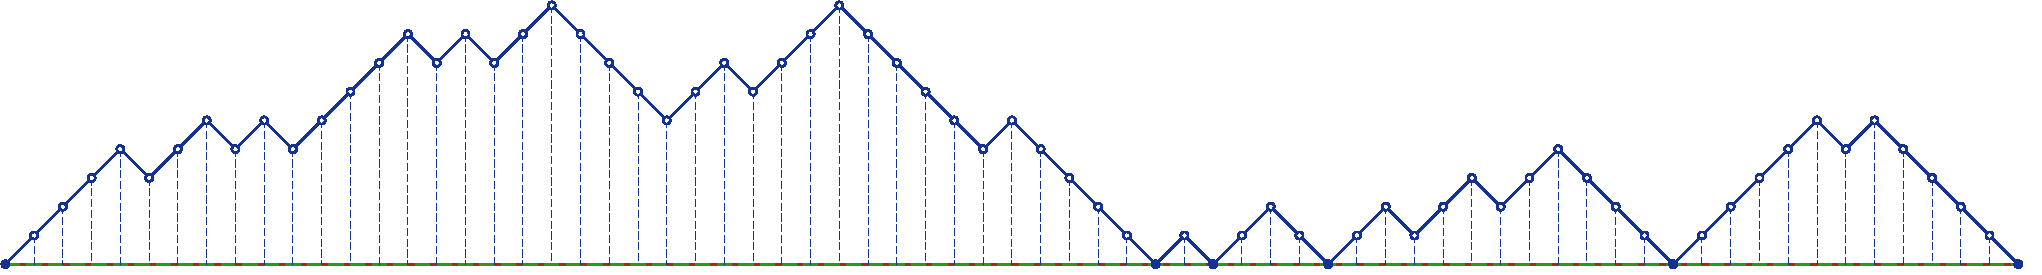
\includegraphics[width=\textwidth]{images/basic_dyck_path.pdf}
    \caption{Simple Dyck path with $n = 35$ up and down steps.}
    \label{fig:basic_dyck}
\end{figure}
One interpretation of Catalan objects is given by Dyck paths (Figure~\ref{fig:basic_dyck}).
A Dyck path is essentially a $2n$ step \emph{balanced} one-dimensional walk with exactly $n$ up and down steps.
In Figure~\ref{fig:basic_dyck}, each step moves one unit along the positive $x$-axis (time) and one unit up or down the positive $y$-axis (position).
The prefix constraint implies that the $y$-coordinate of any point on the walk is $\ge 0$ i.e. the walk never crosses the $x$-axis.
The number of possible Dyck paths (see Theorem~\ref{thm:number_of_dyck_paths}) is the $n^{th}$ Catalan number $C_n=\frac{1}{n+1}\cdot{2n\choose n}$.
Many important combinatorial objects occur in Catalan families of which these are an example.

We will approach the problem of partially sampling Catalan objects through Dyck paths.
This, in turn, will allow us to implement access other random Catalan objects such as rooted trees, and bracketed expressions.
Specifically, we will want to answer the following queries:
\begin{itemize}
    \item \func{Direction}$(t)$: Returns the value of the $t^{th}$ step in the Dyck path (whether the step is up or down).
    \item \func{Height}$(t)$: Returns the $y$-position of the path after $t$ steps
    (the number of up steps minus the number of down steps among the first $t$ steps).
    Since a $\func{Direction}(t)$ query can be simulated using the queries $\func{Height}(t)$ and $\func{Height}(t-1)$,
    we will not explicitly discuss the \func{Direction} queries in what follows.
    \item \func{First-Return}$(t)$: If the $(t+1)^{th}$ step is upwards i.e. $\func{Height}(t+1) = \func{Height}(t)+1$,
    it returns the smallest index $t'>t$ such that $\func{Height}(t')=\func{Height}(t)$.
    While it may not be clear why this query is important, it will be useful for querying bracketed expressions and random trees.
    (see Section~\ref{sec:bijections_to_other_catalan_objects}).
\end{itemize}



\subsection{Bijections to other Catalan objects}%
The $\func{Height}$ query is natural for Dyck paths, but the $\func{First-Return}$ query is important in exploring other Catalan objects.
For instance, consider a random well bracketed expression; equivalently an uniform distribution over the Dyck language.
One can construct a trivial bijection between Dyck paths and words in this language
by replacing up and down steps with opening and closing brackets respectively (Figure~\ref{fig:dyck_bijection}).
The $\func{Height}$ query corresponds to asking for the nesting depth at a certain position in the word,
and $\func{First-Return}(x)$ returns the position after the matched closing bracket for the step $(x\rightarrow x+1)$.

\label{sec:bijections_to_other_catalan_objects}
\begin{figure}[htbp]
    \centering
    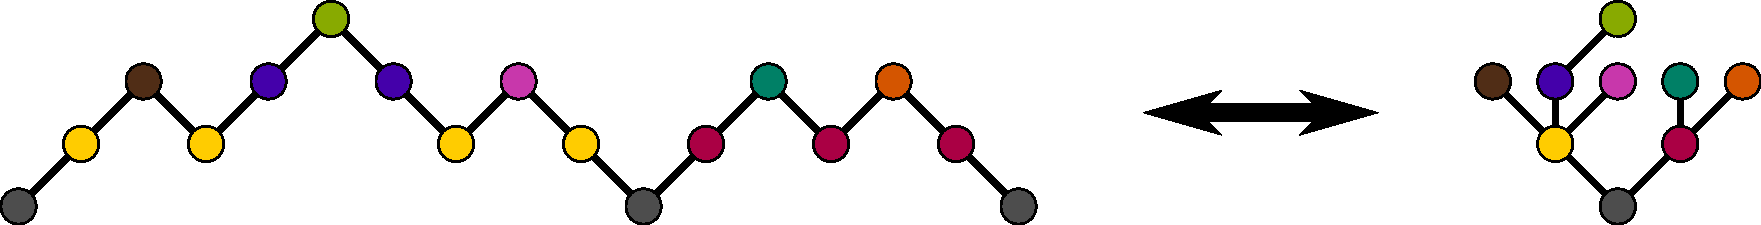
\includegraphics[width=\textwidth]{images/dyck_tree_bijection.pdf}
    \caption{Bijections from Dyck paths to bracketed expressions and ordered rooted trees.
    Note that the color coded \emph{positions} on the path correspond to tree nodes, and the path itself is a DFS traversal of the tree.
    The bijection to bracketed expressions proceeds by directly replacing up and down steps with opening and closing brackets respectively
    (we color the brackets with the \emph{higher} endpoint of the corresponding step).
    Green dashed arrows show successive $\func{First-Return}$ queries on the path.
    Using the bijection, this is equivalent to revealing three child sub-trees in order from left to right for the corresponding tree node,
    and also to finding matching brackets in bracketed expressions.
    \func{First-Return} is not defined for the red boxed nodes in either forward or reverse direction,
    since this position corresponds to a leaf node in the tree, or to a terminal nesting level in the bracket expression.}
    \label{fig:dyck_bijection}
\end{figure}
There is also a natural bijection between Dyck paths and ordered rooted trees (Figure~\ref{fig:dyck_bijection}),
by viewing the Dyck path as a transcript of the tree's DFS traversal.
Starting with the root, for each ``up-step'' we move to a new child of the current node, and for each ``down-step'', we backtrack towards the root.
Thus, the $\func{Height}$ query returns the depth of a node.
Also, since the Dyck path is a DFS transcript of the tree, a $\func{First-Return}$ query on the path
can be used to find successive children of a tree node (each return produces the \emph{next child}).
For instance, in Figure~\ref{fig:dyck_bijection}, we can invoke \func{First-Return} thrice
starting at the first \emph{yellow path position} to reveal the corresponding three children of the \emph{yellow tree node}.
%A similar argument shows a bijection to the set of all ordered binary trees.

By definition, \func{First-Return}$(x)$ is meaningful only when the step from $x$ to $x+1$ is upwards,
i.e. when $\func{Height}(x+1) = \func{Height}(x) + 1$.
We can also implement a \func{Reverse-First-Return} query, which is just a standard \func{First-Return} query on the reversed Dyck path
(consider a reversal of the green dashed arrows in Figure~\ref{fig:dyck_bijection}).
The reversal implies that \func{Reverse-First-Return}$(x)$ is only meaningful when $\func{Height}(x-1) = \func{Height}(x) + 1$.
In terms of bijections, \func{Reverse-First-Return} is equivalent to finding a matching opening bracket in bracketed expressions,
and a \func{Previous-Child} query in rooted trees.
We show how to implement this query in Section~\ref{sec:reverse_first_return_queries}.
In the case where the height at $x$ is larger than both the heights at $x-1$ and $x+1$ (boxed nodes in Figure~\ref{fig:dyck_bijection}),
there is no meaningful ``first return'' from the context of the bijections.
Specifically, these nodes correspond to leaf nodes in rooted trees, or to a terminal nesting level in the bracket expression.

Moving forwards, we will focus on Dyck paths for the sake of simplicity.



\subsection{Catalan Trapezoids and Generalized Dyck Paths}
In order to implement local access to random Dyck paths, we will need to analyze more general Catalan objects.
Specifically, we consider a sequence of $U$ up-steps and $D$ down-steps,
such that any prefix of the sequence containing $U'$ up and $D'$ down steps satisfies $U'-D' \ge 1-k$.
This means that we start our Dyck path at a height of $k-1$, and we are never allowed to cross below zero (Figure~\ref{fig:complex_dyck}).
Note that the case $k=1$ corresponds to the standard description of Dyck paths, as mentioned previously (Figure~\ref{fig:basic_dyck}).
\begin{figure}[htbp]
    \centering
    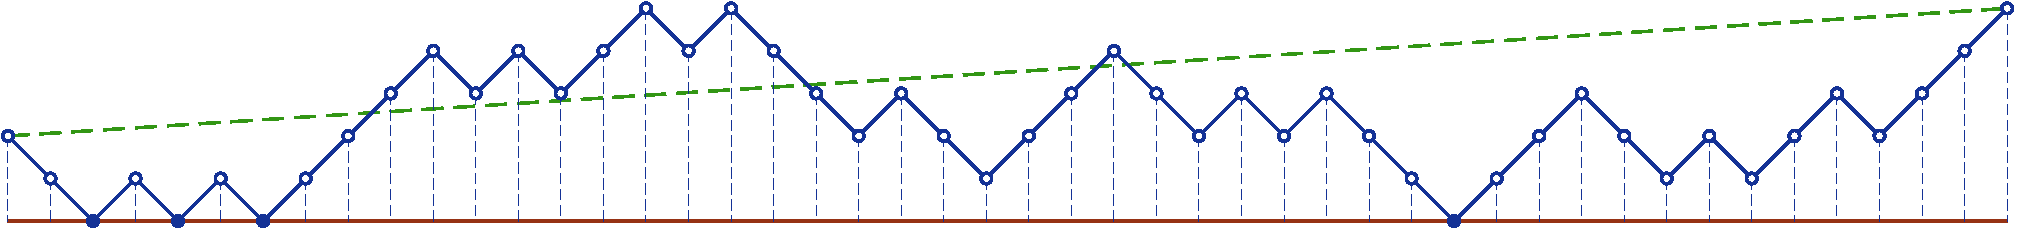
\includegraphics[width=\textwidth]{images/complex_dyck_path.pdf}
    \caption{Generalized Dyck path with $U = 25$, $D = 22$ and $k = 3$.
             Note that the boundary is $k-1 = 2$ units below the starting height.} \label{fig:complex_dyck}
\end{figure}

We will denote the set of such \emph{generalized Dyck paths} as $\mathbb C_k(U,D)$ and the number of paths as $C_k(U,D) = |\mathbb C_k(U,D)|$,
which is an entry in the \textit{Catalan Trapezoid} of order $k$ \cite{trap}.
We also use $\mathsf C_k(U,D)$ to denote the uniform distribution over $\mathbb C_k(n,m)$.
Now, we state a result from \cite{trap} without proof:
\begin{align}
    \label{eq:catalan_trapezoid}
    C_k(U,D)=
    \begin{cases}
    \binom{U+D}{D} &0\le D<k\\
    \binom{U+D}{D} - \binom{U+D}{D-k} &k\le D\le U+k-1\\
    0 &D>U+k-1
    \end{cases}
\end{align}
For $k = 1$ and $n=m$, these represent the vanilla Catalan numbers i.e. $C_n = C_1(n,n)$ (number of simple Dyck paths).
Our goal is to sample from the distribution $\mathsf C_1(n,n)$.

Consider the situation after a sequence of \func{Height} queries to the Dyck path at various locations $\langle x_1, x_2,\cdots, x_m \rangle$,
such that the corresponding heights were sampled to be $ \langle y_1, y_2,\cdots, y_m \rangle$.
These revealed locations partition the path into disjoint \emph{intervals} $[x_i,x_{i+1}]$,
where the heights of the endpoints of each interval have been determined (as $y_i = \func{Height}(x_i)$).
We notice that these intervals can be generated independently of each other.
Specifically, the path within the interval $[x_i, x_{i+1}]$ will be sampled from $\mathsf C_k(U,D)$,
where $k - 1 = y_i$, $U + D = x_{i+1} - x_i$, and $U-D = y_{i+1} - y_i$.
Moreover, since the heights of the endpoints $y_i$ and $y_{i+1}$ are known, this choice is independent of any samples outside the interval.
Next, in Section~\ref{sec:implementing_height_queries}, we will show how one can determine heights within such an interval,
and in Section~\ref{sec:supporting_first_return_queries} we will move on to the more complicated $\func{First-Return}$ queries.

%We also maintain a threshold $\mathcal T = \Theta(\log^4 n)$.
%If a query lands in an interval that has length less than $\mathcal T$, then we brute force  the entire interval one step at a time.
%Assuming that the probabilities of these events can be approximated efficiently (Lemma~\ref{lem:probability_approximation_oracle},
%this take $\poly(\log n)$ time.



\subsection{Implementing \func{Height} queries}
\label{sec:implementing_height_queries}
We implement $\func{Height}(t)$ by showing how to efficiently determine the height of the path
at the midpoint of an existing interval $[x_i, x_{i+1}]$ (with corresponding endpoint heights $y_i, y_{i+1}$),
which results in two sub-intervals that are half the size.
Next, we extend this strategy to determine the heights of arbitrary positions by recursively sub-dividing the relevant interval (binary search).
If the interval in question has odd length, we sample a single step from an endpoint, and proceed with a shortened even length interval.
Sampling a single step is easy since there are only two outcomes (see proof of Theorem~\ref{thm:dyck_midpoint_sampling}).
\begin{figure}[htpb]
    \centering
    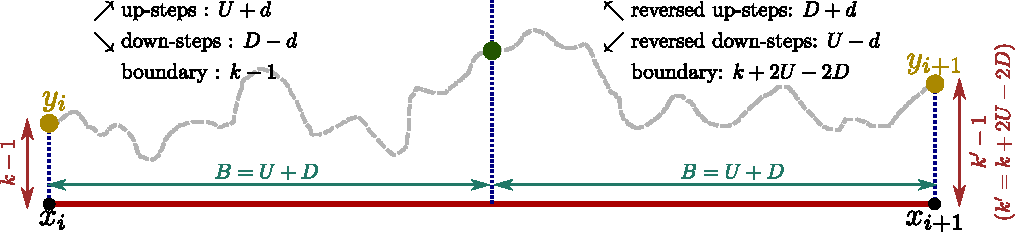
\includegraphics[width=\textwidth]{images/dyck_height_sampling.pdf}
    \caption{The $2B$-interval is split into two equal parts resulting in two separate Dyck problems.
             The green node (center) is the sampled height of the midpoint parameterized by the value of $d$.
             The path considered in both sub-intervals starts at a yellow node (left and right edges) and ends at the green node.
             From this perspective, the path on the right is reversed with up and down steps being swapped.
             A possible path is shown in gray.}
    \label{fig:dyck_height_sampling}
\end{figure}

Our general recursive step is as follows.
We consider an interval of length $2B$ comprising of $2U$ up-steps and $2D$ down-steps where the sum of any prefix cannot be less than $k-1$
i.e. the path within this interval should be sampled from $\mathsf C_k(2U,2D)$.
In order to make the analysis simpler, we have assumed that the number of up and down steps are both even.
The case of sampling according to $\mathsf C_k(2U+1, 2D+1)$ works similarly with slightly different formulae.
Without loss of generality, we assume that $D\le U$; if this were not the case, we could simply flip the interval,
swap the up and down steps, and modify the prefix constraint to $k'=k+2U-2D$ (Figure~\ref{fig:dyck_height_sampling}).
This ensures that the overall path in the interval is non-decreasing in height, which will simpify our analysis.

We determine the height of the path $B = U+D$ steps into the interval at the midpoint (see Figure~\ref{fig:dyck_height_sampling}).
This is equivalent to finding the number of up or down steps that get assigned to the first half of the interval.
We parameterize the possibilities by $d$ and define $p_d$ to be the probability that exactly $U+d$ up-steps and $D-d$ down steps
get assigned to the first half (with the remaining $U-d$ up steps and $D+d$ down steps being assigned to the second half).
\begin{align}
\label{eq:height_sampling_probability}
p_d = \frac{S_{left}(d)\cdot S_{right}(d)}{S_{total}(d)}
\end{align}
Here, $S_{left}(d)$ denotes the number of possible paths in the first half (using $U+d$ up steps)
and $S_{right}(d)$ denotes the number of possible paths in the second half (using $U-d$ up steps).
Note that all of these paths have to respect the $k$-boundary constraint (cannot dip more than $k-1$ units below the starting height), where $k=y_i+1$.
Moving forwards, we will drop the $d$ when referring to the path counts.
We (conceptually) flip the second half of the interval,
such that the corresponding path begins from the end of the $2B$-interval and terminates at the midpoint (Figure~\ref{fig:dyck_height_sampling}).
This results in a different starting point, and the prefix/boundary constraint will also be different.
Hence, we define $k' = k + 2U - 2D$  to represent the new boundary constraint (since the final height of the $2B$-interval is $k'-1$).
Finally, $S_{total}$ is the total number of possible paths in the $2B$ interval.

We cannot directly sample from this complicated distribution $\{ p_d\}$.
Instead, we use the rejection sampling strategy from Lemma~\ref{lem:rejection_sampling}.
An important point to note is that in order to apply this lemma, we must be able to approximate the $p_d$ values.
However, we cannot naively use the formula from Equation~\ref{eq:height_sampling_probability},
since the values of $\{ S_{left},S_{right},S_{total}\}$ are too large to compute explicitly.
Lemma~\ref{lem:probability_approximation_oracle} in Section~\ref{sec:computing_probabilities}
shows how to indirectly compute the probabilty approximations.
We also use the following lemma to bound the deviation of the path with high probability.
A proof is presented in Section~\ref{sec:dyck_path_boundaries_and_deviations}.
\begin{restatable}{lemma}{DyckPathDeviationBound}
\label{lem:DyckPathDeviationBound}
Consider a contiguous \emph{sub-path} of a simple Dyck path of length $2n$
where the sub-path is of length $2B$ comprising of $U$ up-steps and $D$ down-steps (with $U + D = 2B$).
Then there exists a constant $c$ such that the quantities $|B-U|$, $|B-D|$, and $|U-D|$
are all $<c\sqrt{B\log n}$ with probability at least $1-1/n^2$ for every possible sub-path.
\end{restatable}

This lemma allows us to ignore potential midpoint heights that cause a deviation greater than $c \sqrt{B\log n}$.
A direct implication is that with high probability, the correctly sampled value for $d$ will be $\mathcal O(\sqrt{B\log n})$.
In other words, the height of the midpoint takes on one of only  $\mathcal O(\sqrt{B\log n})$ distinct values with high probability.
This immediately suggests a $\widetilde{\mathcal O}(\sqrt{B})$ time algorithm for determining the midpoint height,
by explicitly computing the probabilities of each of these potential heights, and directly sampling from the resulting distribution.
However, we can go further and obtain a $\mathcal O(poly(\log n))$ time algorithm.


\subsubsection{The Simple Case: Far Boundary}%
\label{sec:the_simple_case}
We first consider the case when the boundary constraint is far away from the starting point, i.e. $k$ is large.
The following lemma (proof in Section~\ref{sec:dyck_path_boundaries_and_deviations}) shows that in this case,
we can safely \emph{ignore} the constraint.  Intuitively, this is because the boundary is so far away,
that we do not hit it with high probability even if we choose a random \emph{unconstrained} path.
\begin{restatable}{lemma}{DyckPathIrrelevantBoundary}
\label{lem:dyck_path_irrelevant_boundary}
Given a Dyck path sampling problem of length $B$ with $U$ up, $D$ down steps, and a boundary at $k$,
there exists a constant $c$ such that if $k > c \sqrt{B\log n}$, then the distribution of paths sampled without a boundary $\mathsf C_{\infty}(U,D)$
is $\mathcal O(1/n^2)$-close in $L_1$ distance to the distribution of Dyck paths $\mathsf C_k(U+D)$.
\end{restatable}
By Lemma~\ref{lem:dyck_path_irrelevant_boundary}, the problem of sampling from $C_k(2U,2D)$
reduces to sampling from the hypergeometric distribution $C_{\infty}(2U,2D)$ when $k>\mathcal{O}(\sqrt{B\log n})$
i.e. the probabilities $p_d$ can be approximated by:
\[
q_d = \frac{{{B}\choose{D-d}}\cdot{{B}\choose{D+d}}}{{{2B}\choose{2D}}}
\]
This problem of sampling from the hypergeometric distribution is implemented using $\mathcal O(poly(\log n))$ resources in \cite{huge}
%in the context of interval summable functions
(see Lemma~\ref{lem:ggn_interval_summable} in Section~\ref{sec:multivariate_hypergeometric_sampling}).
We also used this result earlier in the paper in order to find the community assignments in the Stochastic Block Model
(Section~\ref{sec:application_sbm}).

\subsubsection{The Difficult Case: Intervals Close to Zero}
\label{sec:the_difficult_case}
The difficult case is when $k = \mathcal{O}(\sqrt{B\log n})$,
and the previous approximation due to Lemma~\ref{lem:dyck_path_irrelevant_boundary} no longer works.
In this case, we cannot just ignore the boundary constraint, and instead we have to analyze the true probability distribution given by $p_d$.
We obtain an expression for $p_d$ by substituting the formula for generalized Catalan numbers as follows:
(Equation~\ref{eq:catalan_trapezoid}) into Equation~\ref{eq:height_sampling_probability}.
\begin{align}
    S_{left} = C_k(U+d,D-d)
    &&S_{right} = C_{k'}(U-d,D+d)
    &&S_{total} = C_k(2U,2D)
\end{align}
Since the right interval is flipped in our analysis, this changes the prefix/boundary constraint,
and hence, the expression for $S_{right}$ uses $k' = k+2U-2D$.
This also implies that $k' = \Bo(\sqrt{B\log n})$ (using Lemma~\ref{lem:DyckPathDeviationBound}).
We can now use Equation~\ref{eq:height_sampling_probability} to evaluate the probabilties $p_d = S_{left}\cdot S_{right}/S_{total}$.
Recall that $S_{left}$ and $S_{right}$ are the number of possible paths in the left and right half of the interval,
when exactly $U+d$ up steps are assigned to the first half, and $S_{total}$ is the total number of possible paths in the interval.

We will invoke the rejection sampling technique (Lemma~\ref{lem:rejection_sampling}), by constructing a different distribution $q_d$
that approximates $p_d$ up to logarithmic factors over the vast majority of its support
(we ignore all $|d|>\Theta(\sqrt{B\log n})$ since the associated probability mass is negligible by Lemma~\ref{lem:DyckPathDeviationBound}).
In order to perform rejection sampling, we also need good approximations of $p_d$,
which is acheved by Lemma~\ref{lem:probability_approximation_oracle} in Section~\ref{sec:computing_probabilities}.
Next, we define an appropriate $q_d$ that approximates $p_d$ and also has an \emph{efficiently computable} $CDF$.
Surprisingly, as in Section~\ref{sec:the_simple_case}, we will be able to use the hypergeometric distribution for $q_d$,
\[
q_d \equiv \frac{{B\choose D-d}\cdot{B\choose D+d}}{{2B\choose 2D}} = \frac{{B\choose D-d}\cdot{B\choose U-d}}{{2B\choose 2D}}
\]
However, the argument for why this $q_d$ is a good approximation to $p_d$ is far less straightforward.

First, we consider the case where $k\cdot k'\le 2U+1$.
In this case, we use loose bounds for $S_{left} < \binom{B}{D-d}$ and $S_{right} < \binom{B}{U-d}$.
These are true because $\binom{B}{D-d}$ and $\binom{B}{U-d}$ are the total number of \emph{unconstrained} paths
in the left and right half respectively, and adding the boundary constraint can only reduce the number of paths.
We also prove the following lemma in Section~\ref{sec:appendix_implementing_height_queries} to bound the value of $S_{total}$.
\begin{restatable}{lemma}{DTotalFarBoundary}
\label{lem:DTotalFarBoundary}
When $kk' > 2U + 1$, $S_{total} > \frac 12\cdot \binom{2B}{2D}$.
\end{restatable}

Combining the three bounds, we conclude that $p_d < \frac 12 q_d$.
Intuitively, in this case the Dyck boundary is far away, and therefore the number of possible paths
is only a constant factor away from the number of unconstrained paths (see Section~\ref{sec:the_simple_case}).
The case where the boundaries are closer (i.e. $k\cdot k' \le 2U+1$) is trickier,
since the individual counts need not be close to the corresponding binomial counts.
However, in this case we can still ensure that the sampling probability is within poly-logarithmic factors of the binomial sampling probability.
We use the following lemmas to bound $S_{left}$ and $S_{right}$ (proofs in Section~\ref{sec:appendix_implementing_height_queries}).
\begin{restatable}{lemma}{DLeftBound}
\label{lem:DLeftBound}
$S_{left} \le c_1 \frac{ k\cdot\sqrt{\log n}}{\sqrt{B}}\cdot{{B}\choose{D-d}}$ for some constant $c_1$.
\end{restatable}
\begin{restatable}{lemma}{DRightBound}
\label{lem:DRightBound}
$S_{right} \le c_2 \frac{k'\cdot \sqrt{log n}}{\sqrt{B}}\cdot{{B}\choose{U-d}}$ for some constant $c_2$.
\end{restatable}

Finally, we obtain a diferent bound on $S_{total}$ for the \emph{near boundary} case.
\begin{restatable}{lemma}{DTotalNearBoundary}
\label{lem:DTotalNearBoundary}
When $kk' \le 2U + 1$, $S_{total} \ge c_3 \frac{k\cdot k'}{B}\cdot{{2B}\choose{2D}}$ for some constant $c_3$.
\end{restatable}

Multiplying these inequalities together allows us to bound $p_d = S_{left}\cdot S_{right}/S_{total} \le \Theta(q_d\log n)$,
implying $p_d/q_d \le \Theta(\log n)$.
Consequently, we can leverage Lemma~\ref{lem:rejection_sampling} to obtain a sample from $\{ p_d\}$
using $\mathcal O(\log^{\mathcal O(1)}n)$ samples from $\{ q_d\}$,
thus determining the height of the Dyck path at the midpoint of the interval.

\begin{theorem}
\label{thm:dyck_midpoint_sampling}
Given an interval $[x_i,x_{i+1}]$ (and the associated endpoint heights $y_i, y_{i+1}$) in a Dyck path of length $2n$,
with the guarantee that no position between $x_i$ and $x_{i+1}$ has been sampled yet,
there is an algorithm that returns the height of the path at the midpoint of $x_i$ and $x_{i+1}$ (or next to the midpoint if $x_{i+1}-x_i$ is odd).
Moreover, this algorithm only uses $\mathcal O(poly(\log n))$ resources.
\end{theorem}
\begin{proof}
If $x_{i+1}-x_i$ is even, we can set $B = (x_{i+1}-x_i)/2$.
Otherwise, we first sample a single step from $x_i$ to $x_i+1$, and then set $B = (x_{i+1}-x_i-1)/2$.
Since there are only two possibilities for a single step, we can explicitly approximate the corresponding probabilities
using the strategy outlined in the proof of Lemma~\ref{lem:probability_approximation_oracle} (see Section~\ref{sec:computing_probabilities}),
and then sample accordingly.
This allows us to apply the rejection sampling from Lemma~\ref{lem:rejection_sampling}
using $\{ q_d\}$ to obtain samples from $\{ p_d\}$ as defined above.
%Now, if $B > \Theta(\log^2 n)$ we can simply use the rejection sampling procedure described above
%to obtain a $\mathcal O(poly(\log n))$ algorithm.
%Otherwise, we sample each step induividually.
%Since there are only $2B = \Theta(\log^2 n)$ steps, the sampling is still efficient.
\end{proof}

\begin{theorem}
\label{thm:dyck_height_sampling}
There is an algorithm that provides sample access to a Dyck path of length $2n$,
by answering queries of the form \func{Height}$(x)$ with the correctly sampled height of the Dyck path at position $x$
using only $\mathcal O(poly(\log n))$ resources per query.
\end{theorem}
\begin{proof}
The algorithm maintains a successor-predecessor data structure (e.g. Van Emde Boas tree) to store all positions $x$ that have already been determined.
Each newly determined position is added to this structure.
Given a query \func{Height}$(x)$, the algorithm first finds the successor and predecessor (say $a$ and $b$) of $x$ among the already queried positions.
This provides us the guarantee required to apply Theorem~\ref{thm:dyck_midpoint_sampling},
which allows us to query the height at the midpoint of $a$ and $b$.
We then binary search by updating either the successor or predecessor of $x$ and repeat until we determine the height of position $x$.
\end{proof}




\subsection{Supporting ``First Return'' Queries}%
\label{sec:supporting_first_return_queries}
In this section, we discuss more complex queries to a Dyck path.
Specifically, we implement $\func{First-Return}(x)$ to allow the user to query the next time the path returns to \func{Height}$(x)$.
The utility of this kind of query is illustrated through bijections to other random Catalan objects
in Section~\ref{sec:bijections_to_other_catalan_objects}.
An important detail here is that if the first step from $x$ to $x+1$ is an down-step, there is no well defined \func{First-Return}.
%In case of trees, this would correspond to a leaf which has no children.

%We will use the following asymptotic formula for \emph{close-to-central} binomial coefficients
%which will allow us the approximate the probabilities in Section~\ref{sec:estimating_the_cdf}.
%\begin{restatable}{lemma}{CentralBinomialCoefficients}
%\label{lem:CentralBinomialCoefficients}
%(From \cite{asymptopia}) If $k = \frac{n \pm c\sqrt n}{2}$ where $c = o(n^{1/6})$,
%we can approximate $\binom{n}{k}$ up to constant factors by the expression $\frac{2^n}{\sqrt n}\cdot \mathlarger e^{-c^2/2}$.
%\end{restatable}

%Recall that we maintain a threshold $\mathcal T = \Theta(\log^4 n)$ such that
%By setting $\mathcal T = \Theta(\log^4 n)$, we see that for intervals with length $B > \mathcal T$,
%the maximum deviations are bounded by $\mathcal O(\sqrt{B\log n}) = \mathcal O(\log^{2.5}n)$ with high probability.
%This means that if we write the deviation as $c\sqrt B$, we see that $c = \mathcal O(\sqrt{\log n})$ which is $o(B^{1/6})$,
%thus satisfying the condition of Lemma~\ref{lem:CentralBinomialCoefficients}.


\subsubsection{Maintaining a Boundary Invariant}
\label{sec:maintaining_a_boundary_invariant}
Notice that after performing a set of $\func{Height}$ queries $\langle x_1, x_2,\cdots, x_m \rangle$ to the Dyck path,
many different positions are revealed (possibly in adversarial locations).
This partitions the path into at most $m+1$ disjoint and independent \emph{intervals} with known boundary conditions.
The first step towards finding the $\func{First-Return}$ from position $t$ would be to locate the \emph{interval} where the first return occurs.
Even if we had an efficient technique to filter intervals, we would want to avoid considering all $\Theta(m)$ intervals to find the correct one.
In addition, the fact that a specific interval \emph{does not} contain the first return implies dependencies for all subsequent samples.

We resolve these difficulties by maintaining a new invariant.
Consider all positions whose heights have have already been determined, either directly as a result of user given $\func{Height}$ queries,
or indirectly due to recursive $\func{Height}$ calls; $\langle x_1, x_2,\cdots, x_m \rangle$ in increasing order i.e. $x_i<x_{i+1}$.
Let the corresponding heights be $ \langle y_1, y_2,\cdots, y_m \rangle$ i.e. $\func{Height}(x_i) = y_i$.
\begin{invariant}
\label{inv:boundary_invariant}
For any interval $[x_i,x_{i+1}]$ where the heights  of the endpoints have been determined to be $y_i$ and $y_{i+1}$,
and every other height in the interval has yet to determined,
the section of the Dyck path between positions $x_i$ and $x_{i+1}$ is constrained to lie above $min(y_i, y_{i+1})$.
\end{invariant}
\begin{figure}[htpb]
    \centering
    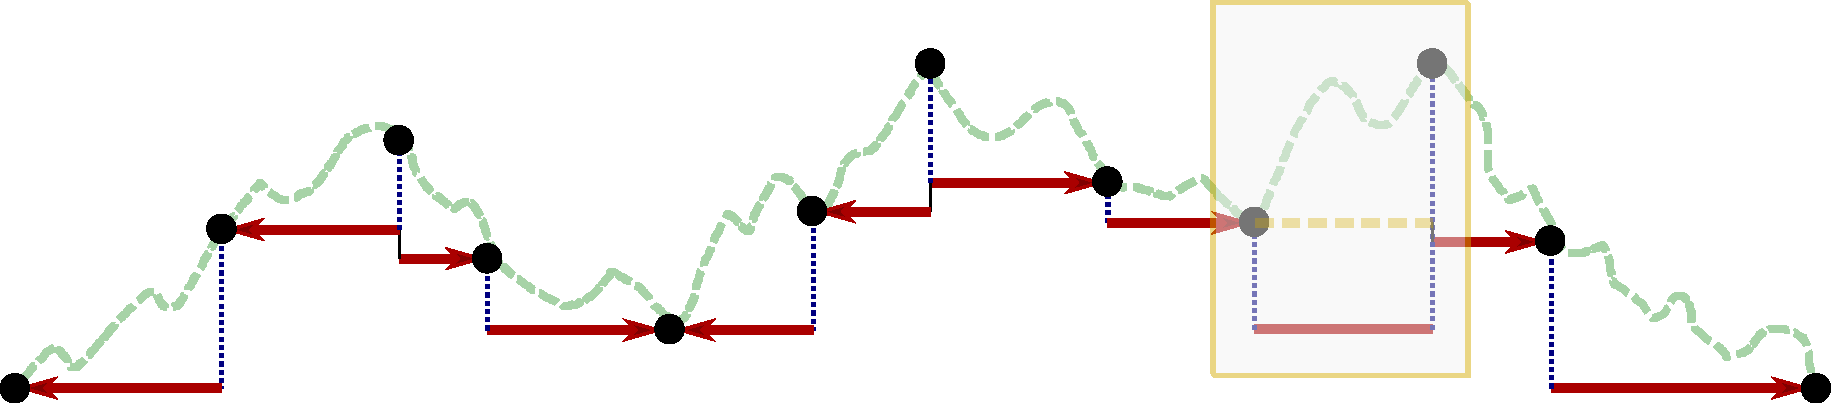
\includegraphics[width=\textwidth]{images/dyck_boundary_invariant.pdf}
    \caption{The set of intervals formed by a set of height samples.
        Each interval also has its own boundary constraint (red).
        Invariant~\ref{inv:boundary_invariant} implies that each boundary must coincide with one of the interval endpoints.
        Note that the only interval which violates the invariant is the third last one (shown in yellow box).}
    \label{fig:dyck_boundary_invariant}
\end{figure}

How can one maintain such an invariant?
After determining the height of a particular position $x_i$ as $y_i$ (with $x_{i-1} < x_i < x_{i+1}$),
the invariant is potentially broken on either side of $x_i$.
We re-establish the invariant by determining the height of an additional point on either side
(see Section~\ref{sec:maintaining_height_queries_under_invariant} for details).
Specifically, we use the following \emph{two step strategy} to find the additional point for some violating interval $[x_i, x_{i+1}]$
(example violation in Figure~\ref{fig:dyck_boundary_invariant}):
\begin{enumerate}
    \item Sample the lowest height $h$ achieved by the walk between $x_i$ and $x_{i+1}$ according to
    the uniform distribution over all possible paths that respect the current boundary constraint
    (see Section~\ref{sec:sampling_the_lowest_achievable_height}).
    \item Find an intermediate position $x$ such that $x_i < x < x_{i+1}$ and $\func{Height}(x) = h$
    (see Section~\ref{sec:sampling_first_position_touching_mandatory_boundary}).
\end{enumerate}
The newly determined position $x$ produces two sub-intervals $[x_i, x]$ and $[x, x_{i+1}]$.
Since $h = \func{Height}(x)$ has been determined to be the minimum height in the overall range $[x_i, x_{i+1}]$,
the invariant is preserved in the new intervals (see Figure~\ref{fig:dyck_invariant_preserve}).
Lemma~\ref{lem:first_return_interval} in Section~\ref{sec:finding_the_correct_interval}
shows how this invariant can help us efficiently search for the interval containing the first return.
\begin{figure}[htpb]
    \centering
    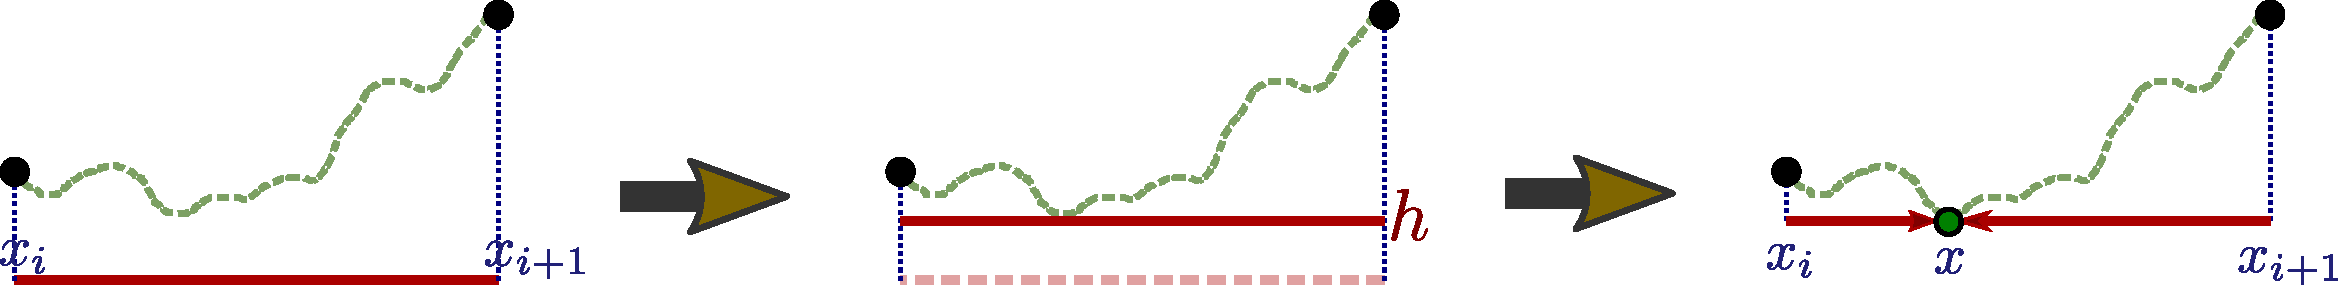
\includegraphics[width=\textwidth]{images/dyck_invariant_preserve.pdf}
    \caption{An interval $[x_i, x_{i+1}]$ that violates the invariant is ``fixed'' by first sampling the lowest height $h$ achieved within the interval,
    and then generating a position $x\in [x_i, x_{i+1}]$ such that $Height(x) = h$.}
    \label{fig:dyck_invariant_preserve}
\end{figure}


\subsubsection{Sampling the Lowest Achievable Height: Mandatory Boundary}
\label{sec:sampling_the_lowest_achievable_height}
First, we need to sample the lowest height $h$ of the walk between $x_i$ and $x_{i+1}$ (with corresponding heights $y_i$ and $y_{i+1}$).
We will refer to $h$ as the \emph{``mandatory boundary''} in this interval;
i.e. no height in the interval may be lower than the boundary, but at least one point \emph{must} touch the boundary (have height $h$).
We assume that $y_i\le y_{i+1}$ without loss of generality; if this is not the case, swap $x_i$ and $x_{i+1}$ and consider the reversed path.
Say this interval defines a generalized Dyck problem with $U$ up steps, $D$ down steps, and a boundary that is $k-1$ units below $y_i$.

Given any two boundaries $k_{lower}$ and $k_{upper}$ on this interval (with $k_{lower} < k_{upper} \le y_i$),
we can count the number of possible generalized Dyck paths that violate the $k_{upper}$ boundary but \emph{not} the $k_{lower}$ boundary as follows
(see Figure~\ref{fig:dyck_mandatory_boundary}):
\[
P_{k_{lower}}^{k_{upper}} = C_{k_{lower}}(U,D) - C_{k_{upper}}(U,D)
\]
\begin{wrapfigure}[16]{r}{0.6\textwidth}
\vspace{-1.5em}
\begin{framed}
    \renewcommand\figurename{Algorithm}
    \caption{Finding the Mandatory boundary}
    \label{alg:mandatory_boundary}
    \begin{algorithmic}[1]
        \Function{Mandatory-Boundary}{$U, D, k$}
            \State {$k_{low}\gets k$}
            \State {$k_{up}\gets 0$}
            \While {$k_{low} < k_{up} - 1$}
                \vspace{.3em}
                \State {$k_{mid}\gets \floor{\frac{(k_{low} + k_{up})}{2}}$}
                \vspace{.3em}
                \State {$P_{total}\gets C_{k_{low}}(U,D) - C_{k_{up}}(U,D)$}
                \vspace{.3em}
                \State {$P_{k_{low}}^{k_{mid}}\gets C_{k_{low}}(U,D) - C_{k_{mid}}(U,D)$}
                \vspace{.3em}
                \State {\textbf{with probability} $P_{k_{low}}^{k_{mid}}/P_{total}$}
                    \State {\hspace{\algorithmicindent}$k_{up}\gets k_{mid}$}
                \State {\textbf{else}}
                    \State {\hspace{\algorithmicindent}$k_{low}\gets k_{mid}$}
            \EndWhile
            \State \Return $k_{low}$
        \EndFunction
    \end{algorithmic}
\end{framed}
\end{wrapfigure}
We define the current lower and upper boundaries as $k_{low} = k, k_{up} = 0$, and set $k_{mid} = (k_{low} + k_{up})/2$.
Since we can compute the quantities $P_{k_{mid}}^{k_{up}}$, $P_{k_{low}}^{k_{mid}}$, and $P_{total} = P_{k_{low}}^{k_{up}}$,
we can sample a single bit to decide if the \emph{``lower boundary''} should move up or if the \emph{``upper boundary''} should move down.
We then repeat this binary search until we find $k' = k_{low} = k_{up}-1$ and $k'$ becomes the \emph{``mandatory boundary''}
(i.e. the walk reaches the height exactly $k'-1$ units below $y_i$ but no lower.
\vspace{2.5em}
\begin{figure}[htpb]
    \centering
    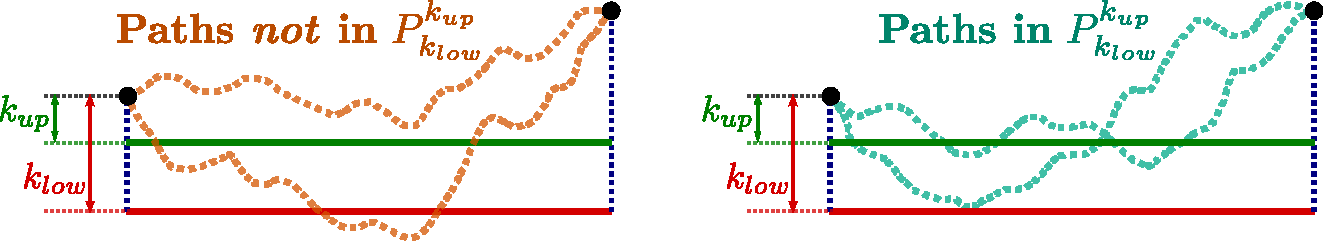
\includegraphics[width=0.9\textwidth]{images/dyck_mandatory_boundary.pdf}
    \caption{$P_{k_{low}}^{k^{up}}$ counts all the paths that dip at least $k_{up}$ units below the starting point,
    but \textbf{do not} dip $k_{low}$ units below the starting point. $k_{mid}$ would lie halfway between these boundaries.}
    \label{fig:dyck_mandatory_boundary}
\end{figure}



\subsubsection{Determining First Position that Touches the \emph{``Mandatory Boundary''}}
\label{sec:sampling_first_position_touching_mandatory_boundary}

Now that we have a ``\emph{mandatory boundary}'' $k$, we just need to generate a position $x\in[x_i,x_{i+1}]$ with $\func{Height}(x) = y_i-k+1$,
according to the uniform distribution over all paths that touch, but do not violate the boundary at $k$.
In fact, we will do something stronger by determining the \emph{first} time the walk touches the boundary after $x_i$.
As before, we assume that this interval contains $U$ up steps and $D$ down steps.
\begin{figure}[htpb]
    \centering
    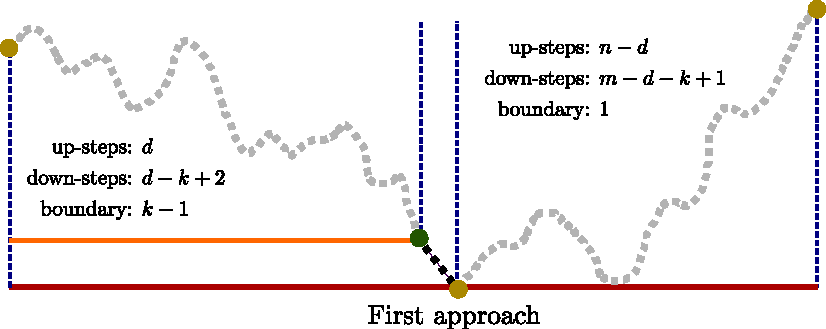
\includegraphics[width=\textwidth]{images/dyck_first_approach_sampling.pdf}
    \caption{Zooming into the error in Figure~\ref{fig:dyck_boundary_invariant}.
        We generate a position $x$ (yellow) on the boundary (red),
        such that the section of the path to the left of $x$ never approaches the red boundary (it respects the orange boundary).}
    \label{fig:dyck_mandatory_boundary_sampling}
\end{figure}

We will parameterize the position $x$ the number of up-steps $d$ between $x_i$ and $x$ (See Figure~\ref{fig:dyck_mandatory_boundary_sampling}).
implying that $x = x_{i} + 2d + k - 1$.
Given a specific $d$, we want to compute the number of valid paths that result in
$d$ up-steps before the first approach to the boundary.
Note that unlike Section~\ref{sec:implementing_height_queries}, $d$ is used here to parameterize the (horizontal) $x$-position of the desired point.
We will calculate the probability $p_d$ associated with a particular position
by counting the total number of paths to the left and right of the first approach and multiplying them together.

As in Section~\ref{sec:the_difficult_case}, we define
$S_{left}$ to be the number of paths in the sub-interval before the first approach (left side of Figure~\ref{fig:dyck_mandatory_boundary_sampling}),
$S_{right}$ to be the number of paths following the first approach,
and $S_{total}$ to be the total number of paths that touch the ``mandatory boundary'' at $k$
(note that these quantities are functions of $U,D,k$ and $d$, but we drop the parameters for the sake of clarity):
{\small
\begin{align*}
    S_{left} = C_{k}(d, d+k-2)
    &&S_{right} = C_1(U-d, D-d-k+1)
    &&S_{total} = C_k(U,D) - C_{k-1}(U,D)
\end{align*}}
Our goal is to generate $d$ from the distribution $\{ p_d\}$ where $p_d = S_{left}\cdot S_{right}/S_{total}$.
The application of Lemma~\ref{lem:rejection_sampling} requires us to approximate $\{p_d\}$
with a ``well behaved'' $\{q_d\}$ (one whose CDF can be efficiently estimated).
Since $q_d$ only needs to approximate $p_d$ up to $\poly(\log n)$ factors,
we focus on obtaining $\poly(\log n)$ approximations to the path counts $\{ S_{left},S_{right},S_{total}\}$.
Using Equation~\ref{eq:catalan_trapezoid}, we obtain approximations for $S_{left}$ and $S_{right}$
(Lemma~\ref{lem:ReturnDLeftBound} and Lemma~\ref{lem:ReturnDRightBound} with proofs in Section~\ref{sec:omitted_supporting_first_return_queries}).
\begin{restatable}{lemma}{ReturnDLeftBound}
\label{lem:ReturnDLeftBound}
If $d > \log^4 n$, then $S_{left}(d)
= \Theta\left( \frac{2^{2d+k}}{\sqrt{d}}\mathlarger e^{-r_{left}(d)}\cdot \frac{k-1}{d+k-1}\right)$
where $r_{left}(d) = \frac{(k-2)^2}{2(2d+k-2)}$.
Furthermore, $r_{left}(d)=\mathcal O(\log^2 n)$.
\end{restatable}

\begin{restatable}{lemma}{ReturnDRightBound}
\label{lem:ReturnDRightBound}
If $U+D-2d-k > \log^4 n$, then $S_{right}(d)
= \Theta\left( \frac{2^{U+D-2d-k}}{\sqrt{U+d-2d-k}}\mathlarger e^{-r_{right}(d)}\cdot \frac{U-D+k}{U-d+1}\right)$
where $r_{right}(d) = \frac{(U-D-k-1)^2}{4(U+D-2d-k+1)}$.
Furthermore, $r_{right}(d)=\mathcal O(\log^2 n)$.
\end{restatable}

Our general strategy will be to integrate continuous versions of these approximations in order to obtain a CDF of some approximating distribution.
Unfortunately, the continuous approximation functions obtained do not admit closed form integrals.
The main culprit is the exponential term in both expressions.
We tackle this issue by noticing that the values of the exponents are bounded by $\mathcal O(\log^2 n)$ over the majority of the range of $d$.
Within this range of $d$ values, the exponential term may be further simplified by taking a piecewise constant approximation,
where each of the pieces corresponds to a fixed value of the \emph{floor of the corresponding exponent}.
This technique is elaborated in Section~\ref{sec:estimating_the_cdf}.

We start by considering the \emph{``problematic''} values of $d$ that are outside the range of the two preceding lemmas.
These values are the ones where $d < \log^4 n$ or $2d > U+D-k-\log^4 n$.
Since $d$ is the number of up steps in the left sub-interval, $d \ge 0$.
Further, since the length of the right sub-interval nust be non-negative (see Figure~\ref{fig:dyck_mandatory_boundary_sampling}),
we get $U+D-2d-k+1 \ge 0$.
Thus, we define the \emph{``problematic''} set:
\begin{align}
\label{eq:SetDefinition}
    \mathcal R = \left\{ d\ \mathlarger|\ 0\le d < \log^4 n \textrm{\textbf{\ or\ }} -1 < 2d-U-D+k < \log^4 n \right\}
\end{align}
Clearly, we can bound the size of this set as $|\mathcal R| = \mathcal O(\log^4 n)$.
An immediate consequence of Lemma~\ref{lem:ReturnDLeftBound} and Lemma~\ref{lem:ReturnDRightBound} is the following.

\begin{restatable}{corollary}{ReturnProbabilityBoundNotNormalized}
\label{cor:ReturnProbabilityBoundNotNormalized}
When $d\not \in \mathcal R$,
$S_{left}(d)\cdot S_{right}(d)
= \Theta\left( \frac{2^{U+D}}{\sqrt{d(U+D-2d-k)}}\cdot \mathlarger e^{-r(d)} \cdot \frac{k-1}{d+k-1}\cdot\frac{U-D+k}{U-d+1}\right)$
where $r(d)=\mathcal O(\log^2 n)$.
\end{restatable}



\subsubsection{Estimating the CDF}
\label{sec:estimating_the_cdf}
We use these observations to construct a suitable $\{q_d\}$ that can be used to invoke the rejection sampling lemma (Lemma~\ref{lem:rejection_sampling}).
We will achieve this by constructing a piecewise continuous function $\hat q$,
such that $\hat q(\delta)$ approximates $p_{\floor\delta}$, and then use the integral of $\hat q$ to define the discrete distribution $\{q_d\}$.
As stated in the previous section, we can leverage the fact that when $d \not \in \mathcal R$,
the floor of the exponent $\floor{r(d)}$ only takes $\mathcal O(\log^2 n)$ distinct values
(consequence of Corollary~\ref{cor:ReturnProbabilityBoundNotNormalized}).
Since the ``problematic'' set $\mathcal R$ only has $\mathcal O(\log^4 n)$ values,
we can also deal with these remaining values by simply creating $|\mathcal R|$ additional continuous pieces in the function $\hat q$.
We begin by rewriting $p_d = \Theta\left(\mathcal K \cdot f(d)\cdot e^{-r(d)}\right)$ where:
{\small
    \begin{align}
    \label{eq:dyck_integrable_function}
        \mathcal K = \frac{2^{U+D}}{S_{total}} = \frac{2^{U+D}}{C_k(U,D)-C_{k-1}(U,D)}\ \ \ \
        &&f(d) = \frac{(k-1)(U-D+k)}{\sqrt{d(U+D-2d-k)}(d+k-1)(U-d+1)}
    \end{align}}
Notice that $\mathcal K$ is a constant and $f(d)$ is a function whose integral has a closed form.
Using the fact that $r(d) = \mathcal O(\log^2 n)$ (Corollary~\ref{cor:ReturnProbabilityBoundNotNormalized}),
and $|\mathcal R| = \mathcal O(\log^4 n)$, we obtain the following lemma:

\begin{lemma}
\label{lem:ReturnProbabilityPiecewiseContinuous}
Given the piecewise continuous function
\begin{align*}
    \hat q(\delta) &=
    \begin{cases}
        p_{\floor\delta} &\mbox{if } \floor\delta \in \mathcal R \\ 
        \mathcal K\cdot f(\delta)\cdot exp\left(-\lfloor{r({\scriptstyle\floor\delta})}\rfloor\right)
        & \mbox{if } \floor\delta \not\in \mathcal R
    \end{cases}
    && \mathlarger \implies
    && p_d = \Theta\left( \int\limits_d^{d+1} \hat q(\delta)\right)
\end{align*}
Furthermore, $\hat q(\delta)$ has $\mathcal O(\log^4 n)$ continuous pieces.
%Note that this integral has a closed form for a fixed value of $\floor{r(d)}$.
\end{lemma}
\begin{proof}
For $d \in \mathcal R$, the integral trivially evaluates to exactly $p_d$.
For $d\not\in \mathcal R$, it suffices to show that $p_d = \Theta\left( \hat q(\delta)\right)$ for all $\delta\in [d,d+1)$.
We already know that $p_d = \Theta\left( \mathcal K\cdot f(d)\cdot e^{-r(d)}\right)$.
Moreover, for any $\delta\in [d,d+1)$, the exponential term $e^{-\floor{r(\floor\delta)}}$ in $\hat q(\delta)$
is within a factor of $e$ of the original $e^{-r(\floor\delta)}$ term.

For all $\mathcal O(\log^4 n)$ values $d\in \mathcal R$, $\hat q(\delta)$ is constant on the interval $[d,d+1]$.
Since $r(d) = \mathcal O(\log^2 n)$ by Corollary~\ref{cor:ReturnProbabilityBoundNotNormalized},
the exponential term $e^{-\floor{r(\floor\delta)}}$ in $\hat q(\delta)$ taken on at most $\mathcal O(\log^2 n)$ values.
Thus, $\hat q$ is continuous for a range of $\delta$ correspoding to a fixed value of $\floor{r(\floor\delta)}$,
and so, we conclude that $\hat q$ is piecewise continuous with $\mathcal O(\log^2 n)$ pieces.
\end{proof}

Now, we have everything in place to define the distribution $\{ q_d\}$ that we will be sampling from.
Specifically, we will define $q_d$ and it's CDF $Q_d$ as follows ($\mathcal N$ is the normalizing factor):
{\small
    \begin{align}
        q_d = \left(\int\limits_d^{d+1} \hat q(\delta)\right)\cdot \frac{1}{\mathcal N}
        && Q_d = \left(\int\limits_0^{d+1} \hat q(\delta)\right)\cdot \frac{1}{\mathcal N}
        && \textrm{where }\ \mathcal N = \int\limits_0^{d_{max}+1} \hat q(\delta)
    \end{align}}
%Here the normalizing factor $\mathcal N$ is $\int_0^{d_{max}+1} \hat q(\delta)$.
To show that these can be computed efficiently, it suffices to show that any integral of $\hat q(\delta)$ can be efficiently evaluated.
This follows from the fact that $\hat q$ is piecewise continuous with $\mathcal O(\log^4)$ pieces (Lemma~\ref{lem:ReturnProbabilityPiecewiseContinuous}),
each of which has a closed form integral (since $f(d)$ defined in Equation~\ref{eq:dyck_integrable_function} has an integral).

%However, we also need to be able to compute the constant $\mathcal K = 2^{U+D} = 2^{U+D}S_{total}$.
%The issue is that this value could be too large to compute.
%We mitigate this by fixing a threshold $\mathcal T = \Theta(\log^4 n)$, and ensuring that $U+D > \mathcal T$.
%In the case that $U+D \le \mathcal T$, we directly compute the $p_d$ values, and sample from the explicit distribution.
%Otherwise, we obtain the following lemma:}
%\begin{lemma}
%\label{lem:ReturnProbabilityConstant}
%If $U+D > \Theta(\log^4 n)$, the quantity $\mathcal K = 2^{U+D} = 2^{U+D}S_{total}$ is bounded
%and can be computed efficiently.
%\end{lemma}
%\begin{proof}
%First, notice that $S_{total} = C_k(U,D) - C_{k-1}(U,D)$ is the number of paths with $U$ up steps and $D$ down steps with a boundary at $k$
%First, we compute a $\left( 1\pm 1/n^2\right)$ multiplicative approximation to $\log_2 S_{total}$,
%by using the strategy in Lemma~\ref{lem:probability_approximation_oracle} (Section~\ref{sec:computing_probabilities}).
%Now, we claim that 
%\end{proof}

\begin{lemma}
\label{lem:ReturnProbabilityPiecewiseContinuousIntegral}
Given the function $\hat q_d$ defined in Lemma~\ref{lem:ReturnProbabilityPiecewiseContinuous},
it is possible to approximate the integral $\int_{d_1}^{d_2+1} \hat q(\delta)$ to a multiplicative factor of $\left( 1\pm \frac{1}{n^2} \right)$,
in $\poly(\log n)$ time for any valid $d_1, d_2\in \mathbb Z$ (the bounds must be such that $d_i \ge 0$ and $U+D-2d_i-k+1 \ge 0$).
\end{lemma}
\begin{proof}
We will compute the integral by splitting it up into $\mathcal O(\log^4 n)$ continuous pieces and then approximating the integral over each piece.
The pieces corresponding to values of $d\in \mathcal R$ can be explicitly computed as $\int_d^{d+1} \hat q(\delta) = p_d$
(recall that we can compute $p_d$ using Lemma~\ref{lem:probability_approximation_oracle} from Section~\ref{sec:computing_probabilities}).

The more interesting pieces are over the range of $\delta$ where $\floor\delta\not\in \mathcal R$.
Such a piece is given by a continuous range of values $[\delta_{min}, \delta_{max}]\subseteq [d_1, d_2+1]$,
such that for any $\delta\in [\delta_{min}, \delta_{max}]$, the value of $\floor{r(\floor{\delta})}$ is a constant $E$.
We begin the calculation of $\hat q(\delta) = \mathcal K\cdot f(\delta)\cdot exp(-E)$,
by first computing a $\left( 1\pm 1/n^3\right)$ multiplicative approximation to $\ln \mathcal K = (U + D)\ln 2 - \ln S_{total}$,
using the strategy in Lemma~\ref{lem:probability_approximation_oracle} (Section~\ref{sec:computing_probabilities}).
Since $f(\delta)$ has a closed form integral (Equation~\ref{eq:dyck_integrable_function}),
we can also compute $F = \int_{\delta_{min}}^{\delta_{max}} f(\delta)$.
Using the fact that the exponent is constant over the range $[\delta_{min},\delta_{max}]$, we can write the logarithm of the integral as:
\[
\ln\left(\ \int\limits_{d_{min}}^{d_{max}} \hat q(\delta)\right) = \ln \left( \mathcal K\cdot e^{-E}\cdot F\cdot\right)
= (U + D)\cdot \ln 2 - \ln S_{total} + \ln F - E
\]
If this value is smaller than $-3\ln n$, we can safely ignore it since it contrbuted less than $1/n^3$ to the probability mass.
On the flipside, the logarithm is guaranteed to be bounded by $\mathcal O(1)$.
This upper bound is a result of the fact that $\int \hat q(\delta) = \mathcal O(\sum p_d) = \mathcal O(1)$,
where both the sum and the integral are taken over the entire \emph{valid} range of $d$.
This means that we can exponentiate to obtain the true value of the piecewise integral up to a multiplicative approximation of $(1\pm 1/n^3)$.
Adding the integrals of all the $\mathcal O(\log^4 n)$ pieces together produces the final desired value of the integral.
\end{proof}


Now, we are finally ready to use Lemma~\ref{lem:rejection_sampling} to sample $d$ from the distribution $\{p_d\}$,
using the efficient sampling procedure for $\{q_d\}$.
The only other requirement is the ability to approximate the $p_d$ values, which follows from Lemma~\ref{lem:probability_approximation_oracle}.
\begin{theorem}
\label{thm:first_return_in_interval}
Given a sub-interval $[x_{i},x_{i+1}]$ of a random Dyck path of length $2n$,
such that the only determined heights in the interval are $y_i=\func{Height}(x_i)$ and $y_{i+1}=\func{Height}(x_{i+1})$,
and a mandatory boundary constraint at $k$,
there exists an algorithm that generates a point $x$ within the interval such that $\func{Height}(x) = y_i-k+1$,
using $\poly(\log n)$ time, random bits, and additional space.
\end{theorem}



\subsubsection{Finding the Correct Interval: $\func{First-Return}$ Query}
\label{sec:finding_the_correct_interval}
As before, consider all positions that have been queried already $ \langle x_1, x_2,\cdots, x_m \rangle$ (in increasing order)
along with their corresponding heights $ \langle y_1, y_2,\cdots, y_m \rangle$.
We wish to find the first return to height $y_i$ after $x_i$ (where $y_i = \func{Height}(x_i)$).
Our strategy begins by using Invariant~\ref{inv:boundary_invariant} to find the interval $\mathcal I = [x_k, x_{k+1}]$
containing $\func{First-Return}(x_i)$.
\begin{figure}[htpb]
    \centering
    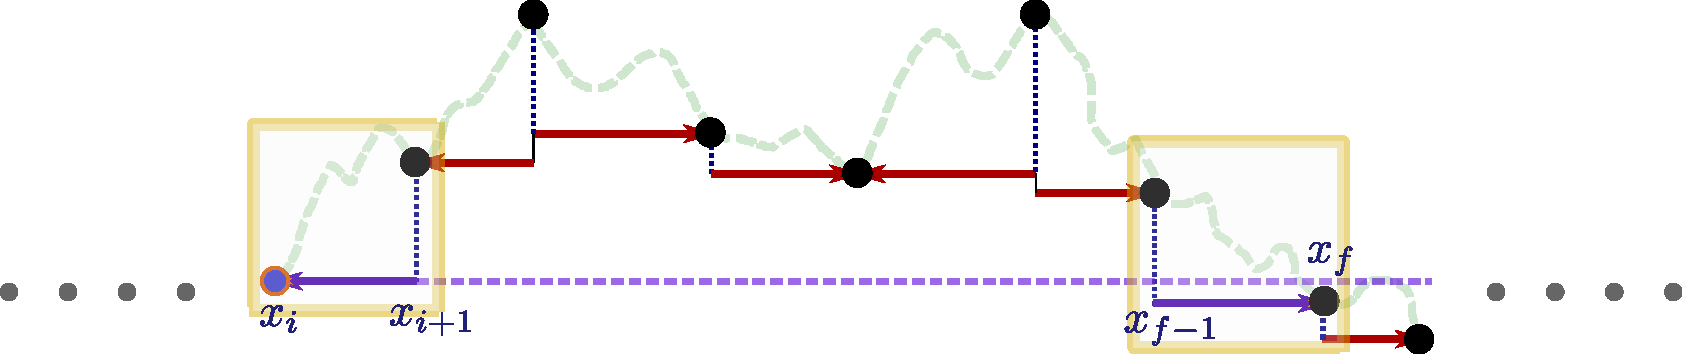
\includegraphics[width=\textwidth]{images/dyck_finding_correct_interval.pdf}
    \caption{There are only two possible intervals (yellow boxes) that could contain $\func{First-Return}(x_i)$;
    either the interval adjacent to $x_i$, or the interval $[x_{f-1}, x_f]$, where $f$ is the smallest index such that $y_f < x_i$.
    }
    \label{fig:dyck_finding_correct_interval}
\end{figure}
\begin{restatable}{lemma}{FirstReturnInterval}
\label{lem:first_return_interval}
Assuming that Invariant~\ref{inv:boundary_invariant} holds, the interval $(x_{j-1},x_{j}]$ containing $\func{First-Return}(x_i)$
is obtained by setting $j$ to be either the smallest index $f>i$ such that $y_f\le y_i$ or setting $j-1=i$.
\end{restatable}
\begin{proof}
We assume the contrary i.e. there exists some $k\not=f$ and $k\not=i+1$ such that the correct interval is $(x_{k-1},x_k]$.
Since $y_f<y_i$, the position of first return to $y_i$ happens in the range $(x_i,x_f]$.
So, the only possibility is $i+1 < k \le f-1$.
By the definition of $y_f$, we know that both $y_k$ and $y_{k-1}$ are strictly larger than $y_i$.
Invariant~\ref{inv:boundary_invariant} implies that the boundary for this interval $(y_{k-1},y_k]$ is at $\min(y_{k-1},y_k) > y_i$.
So, it is not possible for the first return to be in this interval.
\end{proof}

The good news is that there are only two intervals that we need to worry about, one of which is just the adjacent one $[x_i, x_{i+1}]$.
The problem of finding the other interval that may contain the first return boils down to finding the smallest index $f>i$ such that $y_f\le y_i$.
To this end, we define $M_{[a,b]}$ as the minimum determined height in the range of positions $[a,b]$.
%(lowest $y$-value) of any sampled boundary in the range of positions $[a,b]$ along the Dyck path.

One solution is to maintain a range tree $\mathbf R$ \cite{comp_geo} over the range $[2n]$.
Assuming that $2n = 2^l$, we can view $\mathbf R$ as a complete binary tree with depth $r$.
Every non-leaf node is denoted by $\mathbf R_{[a,b]}$, and corresponds to a range $[a,b]\subseteq[2n]$ that is the union of the ranges of its children.
Each $\mathbf R_{[a,b]}$ stores the value $M_{[a,b]}$ which is is the minimum determined height
in the range of positions $[a,b]$, or $\infty$ if none of the heights have been revealed.
%the height of the last boundary update that affected the entire range $[a,b]$.
The leaf nodes are denoted as $\{\mathbf R_i\}_{i\in[2n]}$, and correspond to the singleton range corresponding to position $i\in [2n]$.
%and by definition, this is the min of the values stored at the children of $\mathbf R_{[a,b]}$.
Note that a node at depth $l'$ will correspond to a range of size $2^{l-l'}$, with the root being associated with the entire range $[2n]$.

We say that the range $[a,b]$ is \emph{canonical} if it corresponds to a range of some $\mathbf{R}_{[a,b]}$ in $\mathbf R$.
By the property of range trees, any arbitrary range can be decomposed into a disjoint union of $O(\log n)$ canonical ranges.
We implement $\mathbf{R}$ to support the following operations:
\begin{itemize}
    \item \func{Update}$(x,y)$: Update the height of the position $x$ to $y$.\\
    This update affects all ranges $[a_i,b_i]$ containing $x$.
    So, for each $[a_i,b_i]$ we set $M_{[a_i,b_i]} = \min\left( M_{[a_i,b_i]}, y\right)$.
    \item \func{Query}$(a,b)$: Return the minimum boundary height in the range $[a,b]$.\\
    We decompose $[a,b]$ into $\mathcal O(\log n)$ \emph{canonical} ranges $ \langle r_1, r_2,\cdots\rangle$,
    %For each $r_i$, we compute $M_{r_i}$ as the minimum over all $R_r$ such that the \emph{canonical} range $r$ contains $r_i$.
    %Equivalently, we set $M_{r_i}$ to be the minimum of all values on the path from $\mathbf R_{r_i}$ to the root of $\mathbf R$,
    %which takes $\mathcal O(\log n)$ time.
    %Note that the values stores in the sub-tree rooted at $\mathbf R_{r_i}$ do not affect $M_{r_i}$,
    %since the coreesponding boundary updates did not affect the \emph{entire} range $r_i$ (these updates only affected canonical sub-ranges of $r_i$).
    and return the minimum of all the $M_{r_i}$ values as $M_{[a,b]}$ (since $[a,b]$ is the union of all $r_i$).
\end{itemize}

Now, we can binary search for $f$ by guessing a value $f'$ and checking if $\func{Query}(x_i,x_{f'}) \le y_i$.
Overall, this requires $\mathcal O(\log n)$ calls to $\func{Query}$, each of which makes $\mathcal O(\log n)$ probes to the range tree.
To avoid an initialization overhead, we only create the node $\mathbf{R}_{[a,b]}$ during the first $\func{Update}$ affecting a position $x\in[a,b]$.
Since a call to $\func{Update}$ can create at most $\mathcal O(\log n)$ new nodes in $\mathbf R$,
the additional space required for each $\func{Height}$ or $\func{First-Return}$ query is still bounded.

\begin{theorem}
\label{thm:dyck_first_return_sampling}
There is an algorithm using $\mathcal O(\log^{\mathcal O(1)} n)$ resources per query that provides access to a random Dyck path of length $2n$,
by answering queries of the form \func{First-Return}$(x_i)$ with the correctly sampled smallest position $x'>x_i$,
where the Dyck path first returns to $\func{Height}(x_i)$.
\end{theorem}
\begin{proof}
In order to make the presentation simpler, we ensure that the next determined position after $x_i$ is $x_i+1$ (in other words $x_{i+1} = x_i + 1$).
This can be done by invoking $\func{Height}(x_i+1)$, if needed.
If $\func{Height}(x_i+1) = y_{i+1} < y_i$, we can terminate because $\func{First-Return}(x_i)$ is not defined.
Otherwise, we notice that in this setting, the first return cannot lie in the adjacent interval $[x_i,x_{i+1}] = [x_i, x_i+1]$.

Hence, we proceed to finding the smallest value $f$ such that $y_f \le y_i$, by using the range tree data structure described above.
Since $\func{Height}(x_{f-1}) > y_i \le \func{Height}(x_f)$ by definition,
the interval $(x_{f-1},x_f]$ must contain at least one position at height $y_i$.
We determine the height at the midpoint of this interval,
and then fix the potential violation of Invariant~\ref{inv:boundary_invariant} by finding another point along with its height.
This essentially breaks up the interval $[x_{f-1},x_f]$ into $\mathcal O(1)$ sub-intervals, each at most half the size of the original.
Based on the newly revealed heights, we again find the (newly created) sub-interval containing the first return in $\mathcal O(1)$ time.
We repeat up to $\mathcal O(\log n)$ times, reducing the size of the intervals in consideration, until the position of the first return is revealed.
\end{proof}

\subsubsection{Maintaining \func{Height} Queries under Invariant~\ref{inv:boundary_invariant}}
\label{sec:maintaining_height_queries_under_invariant}
Finally, we show that the boundary constraints introduced in order to maintain Invariant~\ref{inv:boundary_invariant}
do not interfere with the implementation of \func{Height} queries.
As before, we consider the currently revealed heights $ \langle y_1, y_2,\cdots, y_m \rangle$,
along with the corresponding positions $ \langle x_1, x_2,\cdots, x_m \rangle$ (in increasing order).
Say that we are now presented with a a query $\func{Height}(x)$, where $x_i < x < x_{i+1}$.
As in Section~\ref{sec:implementing_height_queries}, we swap $x_i$ and $x_{i+1}$ if necessary in order to ensure that $y_i < y_{i+1}$.
Due to Invariant~\ref{inv:boundary_invariant}, we know that the lowest achievable height in the interval $[x_i, x_{i+1}]$ is $y_i$,
i.e. the boundary constraint for the left half becomes $k = 1$ instead of $k = y_i + 1$, since the constrained boundary is at height $y_i$.
Similarly, the boundary constraint for the right half becomes $k' = 2U - 2D + 1$.

The algorithm for determining the height at the midpoint $x_{mid}$ of $[x_i,x_{i+1}]$
can proceed as described in Section~\ref{sec:implementing_height_queries}.
Of course, in this scenario, the boundary is never far away, and therefore we should always use the strategy in Section~\ref{sec:the_difficult_case}.
The second step is to re-establish Invariant~\ref{inv:boundary_invariant} in the newly created sub-interval $[x_{mid},x_{i+1}]$\footnote{
Note that the invariant is not broken for the $[x_i,x_{mid}]$ sub-interval since $y_i+1$ was the original boundary constraint.
In general, the invariant will be automatically preserved for one of the sub-intervals; the side corresponding to $\min(y_i,y_{i+1})$.},
using the two step strategy from Section~\ref{sec:maintaining_a_boundary_invariant}.
This involves determining the height of one additional point $x'\in [x_{mid},x_{i+1}]$.
Finally, we can continue with the height sampling algorithm from Theorem~\ref{thm:dyck_height_sampling},
by recursively halving one of the newly created intervals (the one containing $x$).
Figure~\ref{fig:dyck_invariant_height_queries} illustrates the aforementioned three steps.
\begin{figure}[htpb]
    \centering
    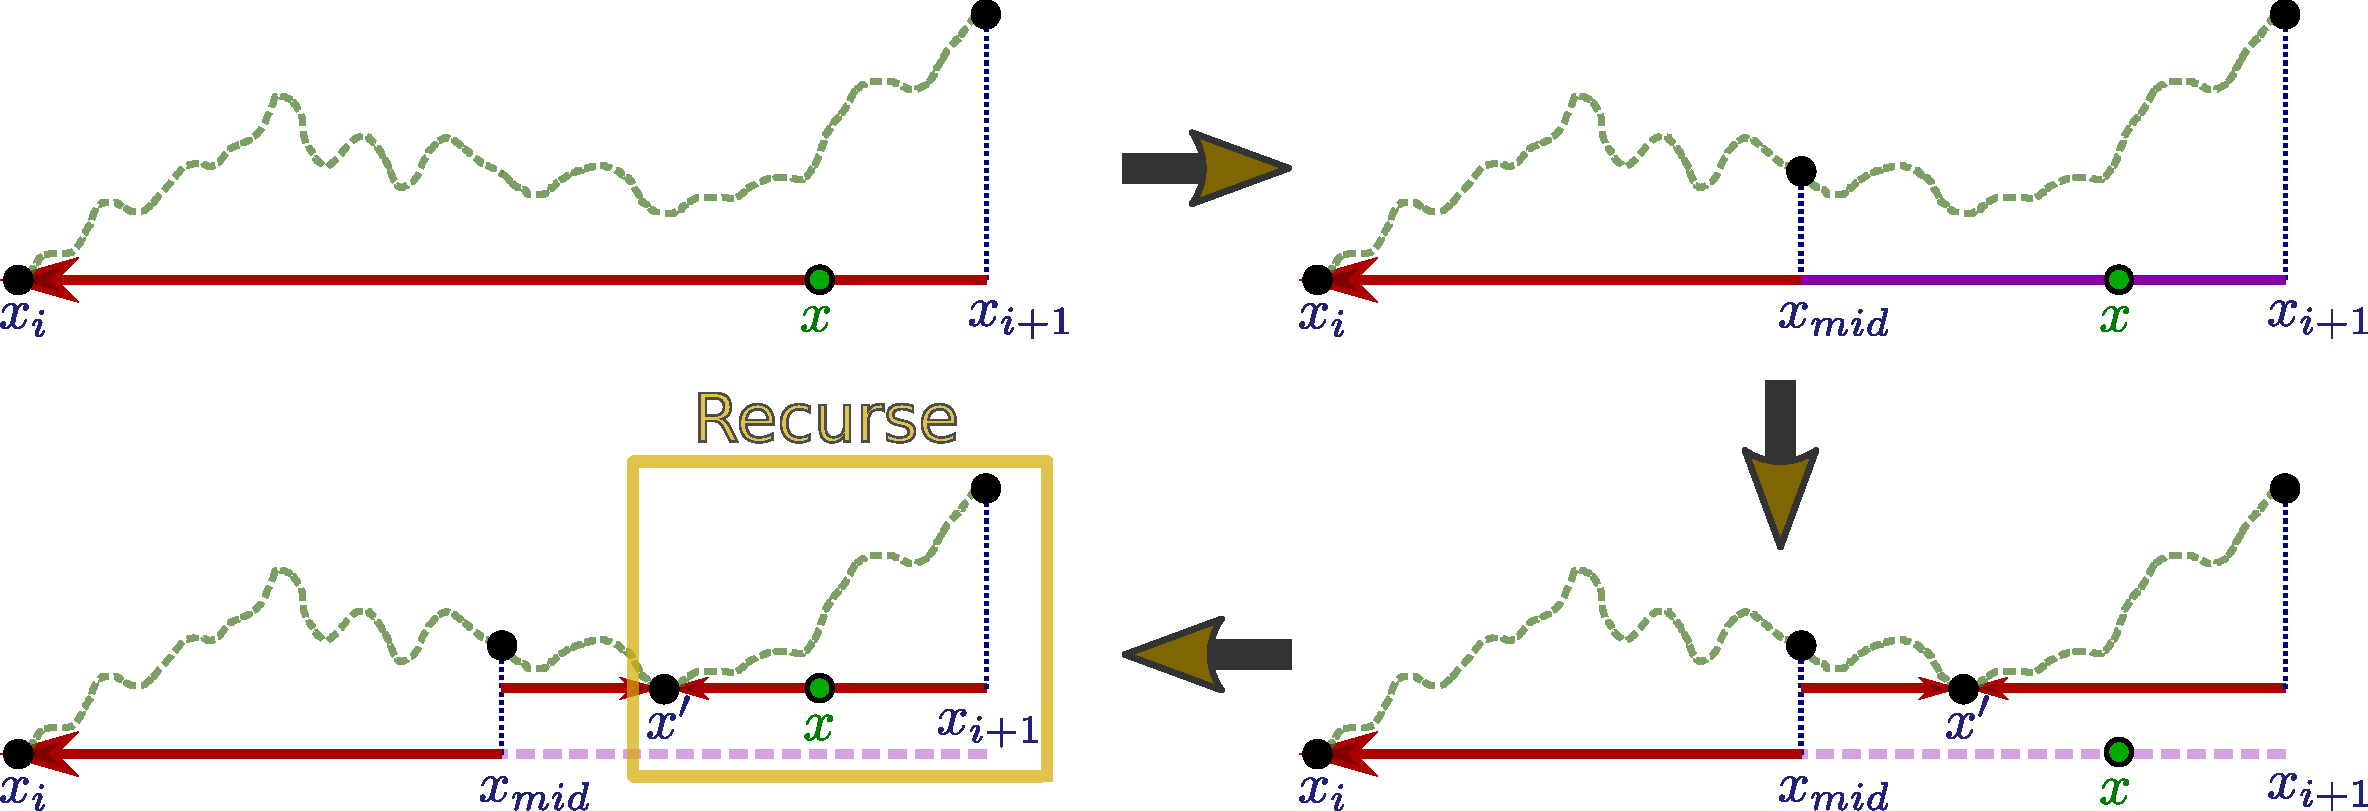
\includegraphics[width=\textwidth]{images/dyck_invariant_height_queries.pdf}
    \caption{Performing \func{Height} queries while maintaining Invariant~\ref{inv:boundary_invariant}.
    The first step is to determine the height at the midpoint $x_{mid}$ of an existing interval $[x_i,x_{i+1}]$ that contains $x$.
    Next, we re-establish Invariant~\ref{inv:boundary_invariant} by sampling an additional point $x'$ within the violating interval
    Finally, we recurse on the appropriate sub-interval (yellow box).
    }
    \label{fig:dyck_invariant_height_queries}
\end{figure}

Hence, we can combine results from Theorem~\ref{thm:dyck_height_sampling} and Theorem~\ref{thm:dyck_first_return_sampling} to obtain the following:
\CatalanGrand*


\subsubsection{\func{Reverse-First-Return} Queries}
\label{sec:reverse_first_return_queries}
For the sake of completeness, we also sketch how to implement a \func{Reverse-First-Return} query,
which is just a standard \func{First-Return} query on the reversed Dyck path.
This type of query was motivated in Section~\ref{sec:bijections_to_other_catalan_objects},
and can be applied to positions $x$ where $\func{Height}(x-1) = \func{Height}(x)+1$.

Note that Invariant~\ref{inv:boundary_invariant} remains unchanged as it is symmetric to reversal of the Dyck path.
Specifically, the invariant on a particular interval does not change if we swap the endpoints of the interval.
First, we can find the correct interval containing $\func{Reverse-First-Return}(x)$, by using an analog of Lemma~\ref{lem:first_return_interval}.
\begin{restatable}{lemma}{ReverseFirstReturnInterval}
\label{lem:reverse_first_return_interval}
Assuming Invariant~\ref{inv:boundary_invariant}, the interval $[x_{j},x_{j+1})$ containing $\func{Reverse-First-Return}(x_i)$
is obtained by setting $j$ to be either the largest index $f<i$ such that $y_f\le y_i$ or setting $j+1=i$.
\end{restatable}
Since the range tree defined in Section~\ref{sec:finding_the_correct_interval} allows us to query the minimum in arbitrary contiguous ranges,
we can also use it to find the appropriate $f$ for Lemma~\ref{lem:reverse_first_return_interval} through binary search.
Once we have found an interval that is known to contain the \func{Reverse-First-Return},
we can follow the strategy from the proof of Theorem~\ref{thm:dyck_first_return_sampling};
recursively sub-dividing the relevant interval and finding the newly created sub-interval that contains the return,
until we converge on the correct return position.

\section{Domino Tiling the $2\times n$ grid}
We will consider the problem of tiling a square grid with dominos.
This problem has a long history and various importtant applications in statistical physics.
Specifically, we will focus on the local generation of domino tilings of a $2\times n$ grid from the uniform distribution.
The queries will be as an index, and the generator should report the orientation of the domino at the $i^{th}$ position in the grid.
%\begin{figure}[htbp]
    %\centering
    %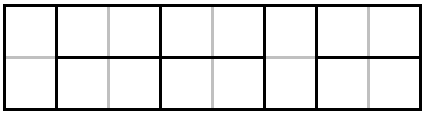
\includegraphics[width=\textwidth]{images/domino2.png}
    %\caption{}
    %\label{fig:dom2}
%\end{figure}

It is a well known result \todo{cite} that the number of tilings of a $2\times n$ grid is exactly $F_n$.
To aid with generalization, we will instead allow the generator to respond with the splitting boundary of the current tiling instead.
For example, in Figure~\ref{fig:b20}, the boundary is a vertical line at the specified position.
In Figure~\ref{fig:b21}, the boundary is horizontal, indicating that there are two horizontal dominos at that location.
Note that Figure~\ref{fig:b22} is impossible for a $2\times n$ grid.
It should be clear that this query model is equivalent.

\begin{figure}[h]
    \centering
    \begin{subfigure}[b]{0.4\textwidth}
        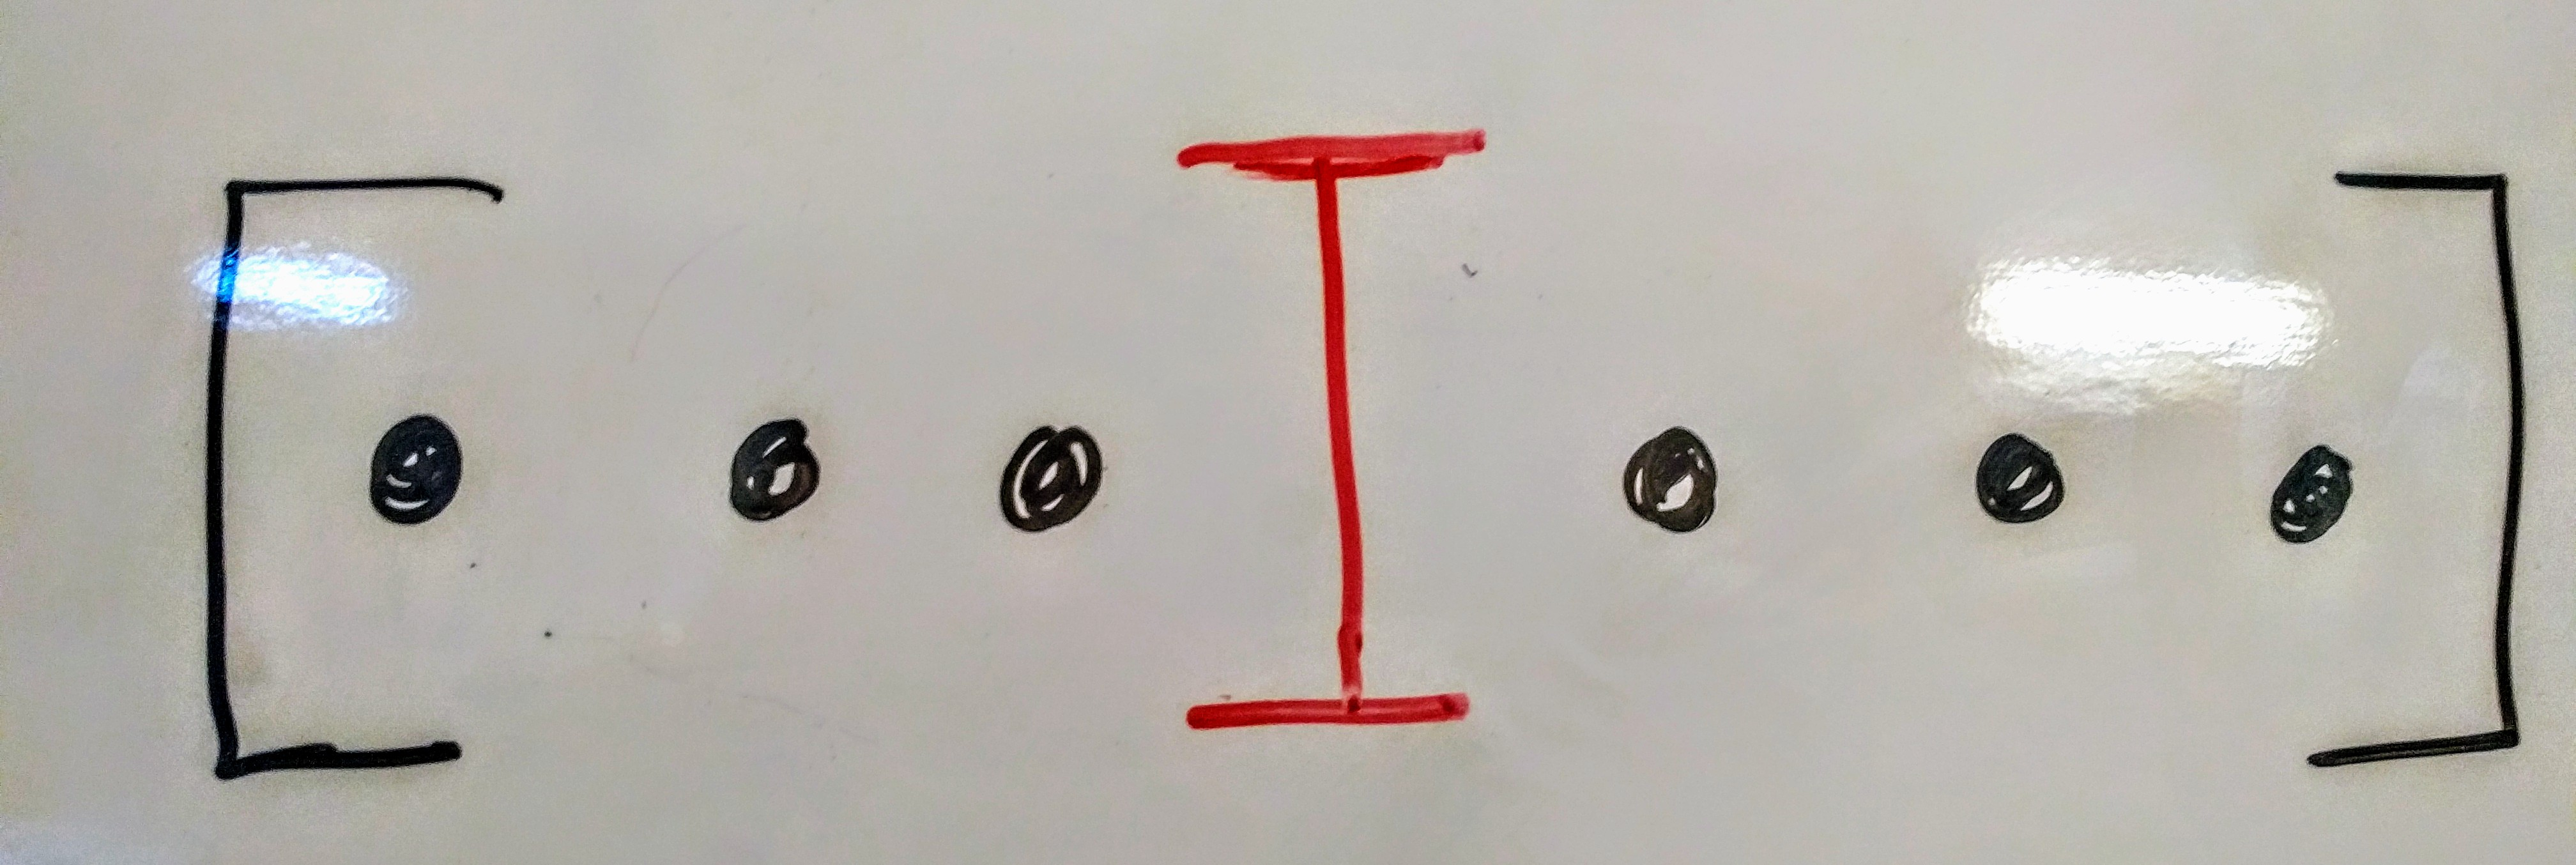
\includegraphics[width=\linewidth]{images/tile2-0.jpg}
        \label{fig:b20}
    \end{subfigure}
    \begin{subfigure}[b]{0.4\textwidth}
        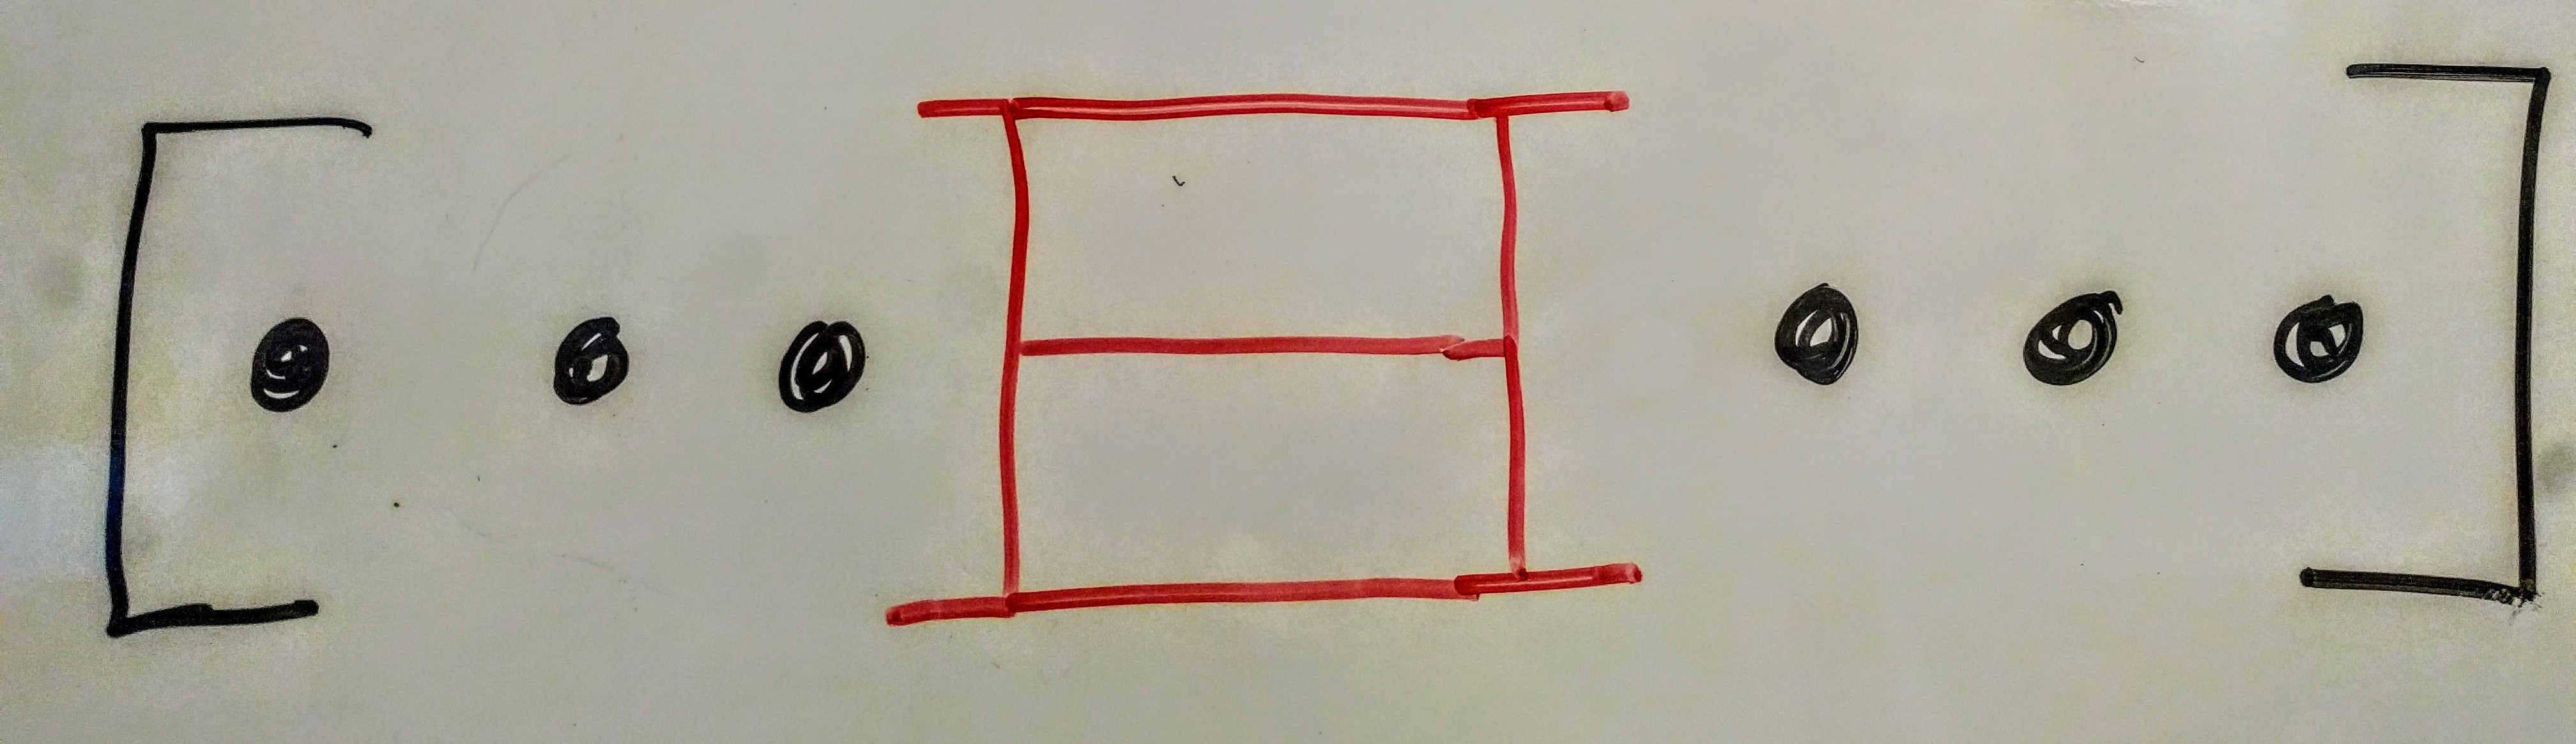
\includegraphics[width=\linewidth]{images/tile2-1.jpg}
        \label{fig:b21}
    \end{subfigure}

    \begin{subfigure}[b]{0.5\textwidth}
        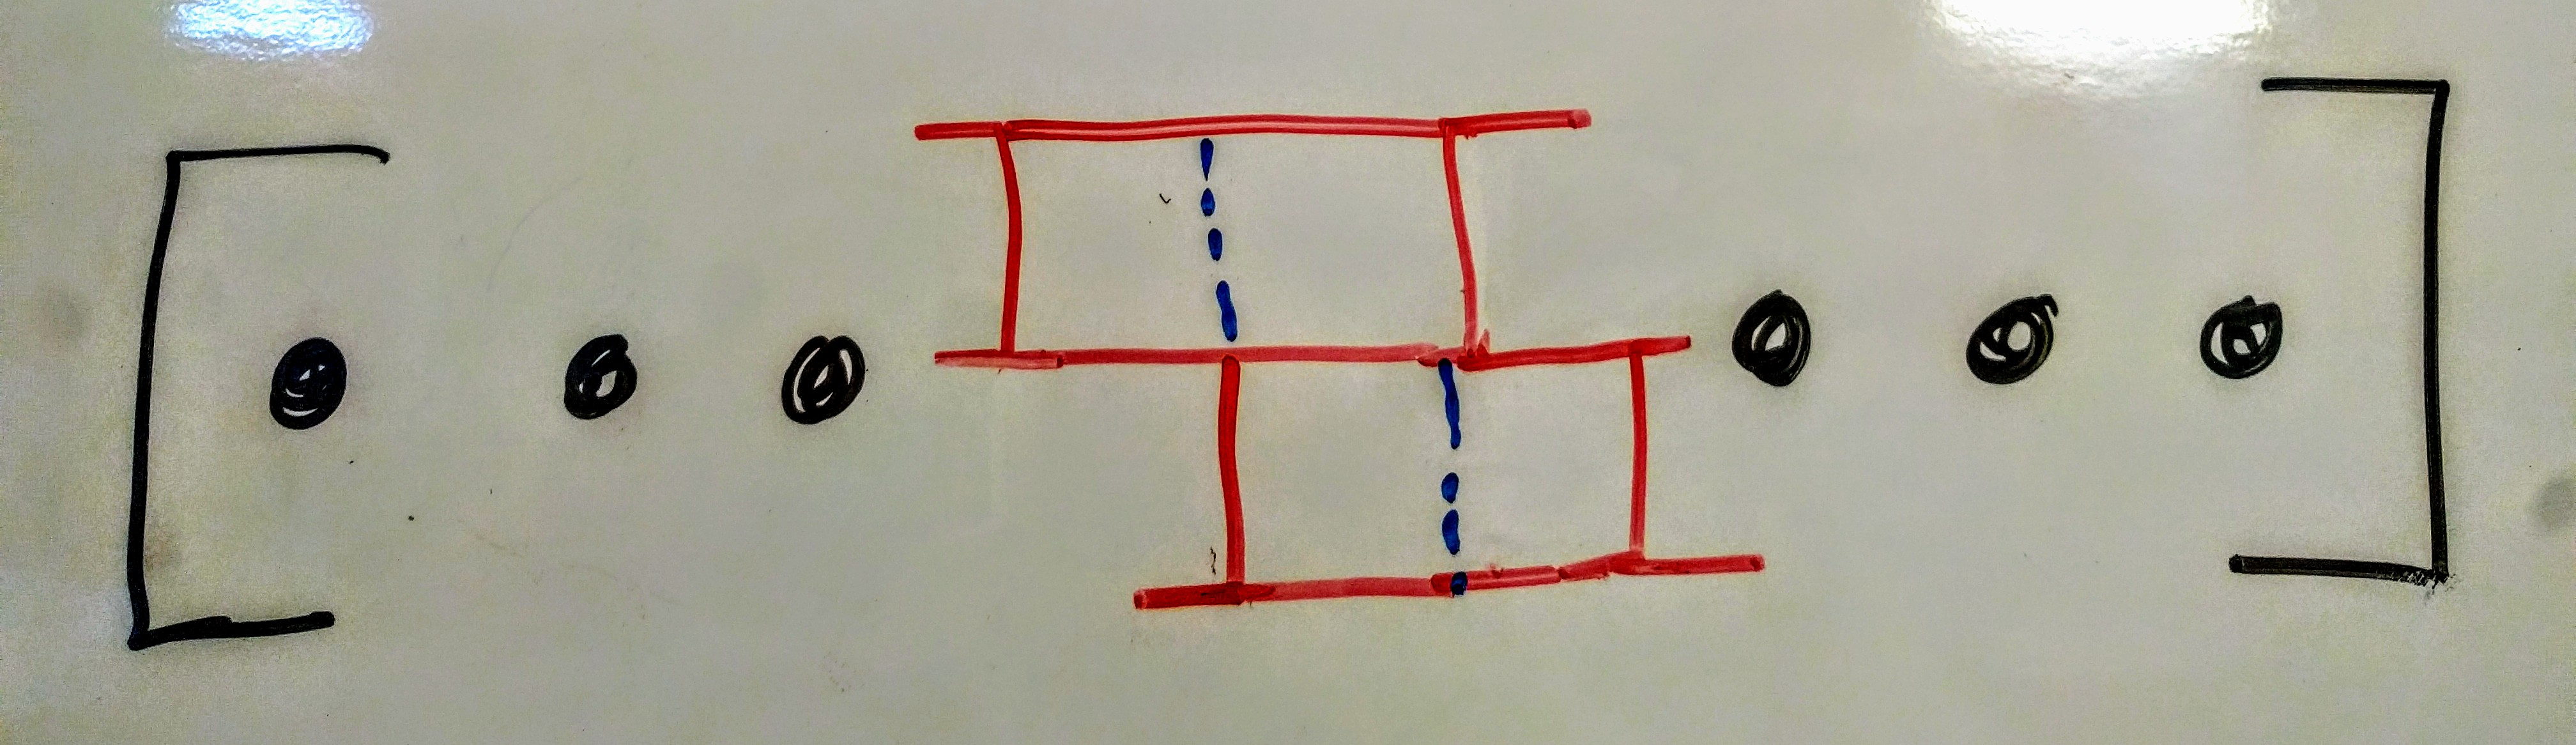
\includegraphics[width=\linewidth]{images/tile2-2.jpg}
        \label{fig:b22}
    \end{subfigure}
    \caption{Caption for this figure with two images}
    \label{fig:boundary2}
\end{figure}

Now, consider a query to the location $i$, such that all positions between $i-a$ and $i+b$ have not been queriesd so far.
So, there is a blank $2\times(a+b)$ size sub-grid that we have to sample from.
Let us consider the number of possible tilings resulting from each possible splitting boundary.
\begin{enumerate}
    \item Vertical Boundary -- This indicates that we divide the region into two sub-grids with sizes
          $2\times a$ and $2\times b$.
          So, the total number of possible tilings is exactly $F_a\cdot F_b$.
    \item Horizontal Boundary -- This indicates that we divide the region into two sub-grids with sizes
          $2\times (a-1)$ and $2\times (b-1)$.
          So, the total number of possible tilings is exactly $F_{a-1}\cdot F_{b-1}$.
\end{enumerate}

So the probabilities are computed as $\frac{F_a\cdot F_b}{F_a\cdot F_b + F_{a-1}\cdot F_{b-1}}$
and $\frac{F_{a-1}\cdot F_{b-1}}{F_a\cdot F_b + F_{a-1}\cdot F_{b-1}}$.
Now, we face the issue of approximating these fractions.
If either of the values $a$ or $b$ are less than $\Theta(\sqrt n)$,
then we can compute the exact value of the corresponding $F_a$ or $F_b$.
Otherwise, we use Lemma~\ref{lem:rat_conv} to approximate $F_a=\phi\cdot F_{a-1}$ and $F_b=\phi\cdot F_{b-1}$.
So, the probability of the vertical boundary becomes
$$
\frac{F_a\cdot F_b}{F_a\cdot F_b + F_{a-1}\cdot F_{b-1}} = \frac{\phi^2}{\phi^2+1}
$$
Similarly, the probability of a horizontal split with a top and bottom domino becomes $1/(\phi^2+1)$.
Note that this also determines the two adjacent boundaries.

The only information we needed to make this query was the extent of the un-queried interval $[i-a, i+b]$.
We can use any standard data-structure that allows insertion in positions $\{1, 2\cdots,n+1\}$,
and provides successor and predecessor queries.

Here's we can be fancy and use Van-Emde-Boas trees to get a $\Bo(\log\log n)$ query time.
However, in some cases, the exact value of a Fibonacci number still needs to be computed, and this takes $\Bo(\log n)$ time.
The faster queries only work when the new query is "far enough" ($\Bo(\log n)$ distance) away from all previous queries.


\section{Random Coloring of a Graph}%
\label{sec:random_coloring_of_a_graph}

\todo{Query access}
We wish to locally sample an uniformly random coloring of a graph.
A $q$-coloring of a graph $G = (V, E)$ is a function $\sigma : V\rightarrow [q]$,
such that for all $(u,v)\in E$, $\sigma_u \not= \sigma_v$.
We will consider only bounded degree graphs, i.e. graphs with max degree $\le \Delta$.
Otherwise, the coloring problem becomes NP-hard\todo{cite}.

Using the technique of path-coupling, Vigoda \todo{cite} showed that for $q > 2\Delta$,
one can sample an uniformly random coloring by using a MCMC algorithm.

The Markov Chain proceeds in $T$ steps. The state of the chain at time $t$ is given by $\vec X^t\in [q]^{|V|}$.
Specifically, the color of vertex $v$ at step $t$ is $\vec X^t_v$.

In each step of the Markov process, a pair $(v, c)\in V\times [q]$ is sampled uniformly at random.
Subsequently, if the recoloring of vertex $v$ with color $c$ does not result in a conflict with $v$'s neighbors,
i.e. $c\not\in \left\{ X^t_u : u\in \Gamma(v)\right\}$, then the vertex is recolored i.e. $X_v^{t+1}\leftarrow c$.

After running the MC for $T = \mathcal{O}(n\log n)$ steps we reach the stationary distribution ($\epsilon$ close),
and the coloring is an uniformly random one.

\textbf{Exact Bound:}
$t_{mix}(\epsilon) \le \left( \frac{q-\Delta}{q-2\Delta}\right)n\left( \log n + \log(1/\epsilon)\right)$
\todo{cite book (Peres, Lyons)}



\subsection{Modified Glauber Dynamics}%
\label{sec:modified_glauber_dynamics}

Now we define a modified Markov Chain as a special case of the \emph{Local Glauber Dynamics} presented in \cite{mohsen}.
The modified Markov chain procceds in epochs.
We denote the initial coloring of the graph by $\vec X^0$ and the state of the coloring after the $k^{th}$ epoch by $\vec X^k$.
In the $k^{th}$ epoch $\mathcal E_k$:
\begin{itemize}
    \item Sample $|V|$ colors $ \langle c_1, c_2,\cdots, c_n \rangle$ from $[q]$, where $c_v$ is the proposed color for vertex $v$.
    \item For each vertex $v$, we set $\vec X^k_v$ to $c_v$ if for all neighbors $w$ of $v$, $\vec X^k_w\not=c_v$ and $\vec X^{k-1}_w\not=c_v$.
\end{itemize}
%\begin{itemize}
    %\item Pick a random permutation $\pi^{(i)}$ of the vertices $V$.
    %\item Sample $n = |V|$ colors $ \langle c_1, c_2,\cdots, c_n \rangle$ from $[q]$.
    %\item Perform the standard update using the pairs $\left\langle (\pi^{(i)}_1, c_1), (\pi^{(i)}_2, c_2), \cdots, (\pi^{(i)}_n, c_n)\right\rangle$.
%\end{itemize}

This procedure is a special case of the \emph{Local Glauber Dynamics} presented in \cite{mohsen}.
The goal in \cite{mohsen} is to find a simultaneous update rule that causes few conflicts among neighbors (and converges to the correct distribution).
Notice that we \emph{can} have adjacent nodes update in the same epoch.
However for the sake of succinctness we use their update rule and avoid a tedious path coupling argument.

\todo{Cite Path Coupling}

We can directly use the path coupling argument from \cite{mohsen} which be briefly describe below.
Given two colorings $\vec X$ and $\vec Y$, we define $d(\vec X,\vec Y)$ as the number of vertices $v$ such that $\vec X_v\not= \vec Y_v$.
We define the coupling $(\vec X,\vec Y)\rightarrow(\vec X',\vec Y')$ where $\vec X$ and $\vec Y$
differ only at a single vertex $v$ such that $\vec X_v = c_X$ and $\vec Y_v = c_Y$.
Now, we pick a random permutation of the vertices along with uniformly sampled colors:
\[
\left\langle (v_1, c_1), (v_2, c_2), \cdots, (v_n, c_n)\right\rangle
= \left\langle (\pi_1, c_1), (\pi_2, c_2), \cdots, (\pi_n, c_n)\right\rangle
\]
Now, for each $(v_i, c_i)$ in order, we update the coloring of $X$ and $Y$ as follows:
\begin{itemize}
    \item If the current color of $v_i$ as well as $c_i$ are both in $\{c_X,c_Y\}$,
    then the $\vec X$ chain picks the color $c_i$ and the $\vec Y$ chain picks the other color.
    \item Otherwise, both chains pick the same color $c_i$ for the vertex $v_i$.
\end{itemize}
We use the following result from \cite{mohsen} that bounds the coupled distance.
\begin{lemma}
\label{lem:mohsen_single_epoch_distance}
If $q = 2\alpha\Delta$ and $d(\vec X, \vec Y) = 1$,
then $\mathbb E[d(\vec X',\vec Y')] \le 1-\left( 1-\frac1{2\alpha}\right)e^{-3/\alpha} + \frac{1/2\alpha}{1-1/\alpha}$
\end{lemma}
\begin{corollary}
\label{cor:single_epoch_distansce}
If $q \ge 9\Delta$ and $d(\vec X, \vec Y) = 1$, then $\mathbb E[d(\vec X',\vec Y')] < \frac1{e^{1/3}}$
\end{corollary}

\begin{theorem}
\label{thm:modified_mixing_time}
If $q\ge 9\Delta$, then the chain is mixed after $\tau_{mix}(\epsilon) = 3\left( \ln n + \ln(\frac1{\epsilon})\right)$ epochs.
\end{theorem}
\begin{proof}
Starting for a maximum distance of $n$, the distance decreases to $1$ after at most $3\ln n$ epochs,
and it takes a further $3\ln\left( \frac{1}{\epsilon} \right)$ to reduce the distance to $\epsilon$.
\end{proof}




\subsection{Local Coloring Algorithm}%
\label{sec:local_coloring_algortihm}
Given query access to the adjacency matrix of a graph $G$ with maximum degree $\Delta$ and a vertex $v$,
the algorithm has to output the color of $v$ after running $t = \mathcal O(\ln n)$ epochs of \emph{Modified Glauber Dynamics}.
We will define the number of colors as $q = 2\alpha\Delta$ where $\alpha > 1$.

The proposals at each epoch are a vector of color samples $\vec C^{t} \thicksim_{\mathcal U} [q]^n$,
where $\vec C^t_v$ is the color proposed by $v$ in the $t^{th}$ epoch.
Note that these values are fully independent and as such any $\vec C^t_v$ can be sampled trivially.
We also use $\vec X^t$ to denote the final vector of vertex colors at the end of the $t^{th}$ epoch.
Finally, we define indicator variables $\bm \chi^t_v$ to denote if the color $\vec C^t_v$ proposed by vertex $v$ was accepted at the $t^{th}$ epoch;
$\bm \chi^t_v = 1$ if and only if for all neighbors $w\in \Gamma(v)$,
we satisfy the condition $\vec C^t_v\not= \vec X^{t-1}_w$ and $\vec C^t_v\not= \vec C^t_w$.
So, the color of a vertex $v$ after the $t^{th}$ epoch $\vec X^t_v$ is set to be $\vec C^i_v$
where $i\le t$ is the largest index such that $\bm \chi^i_v=1$.
While the proposals $\vec C^t_v$ are easy to sample, it is much less clear how we can sample the $\bm \chi^t_v$ values.
Note that we can compute $\vec X^t_v$ quite easily if we know the values $\bm\chi^i_v$ for all $i\le t$.
So, we focus our attention on the query $\func{Accepted}(v,t)$ that returns $\bm\chi^t_v$.


\subsubsection{Naive Coloring Implementations}%
\label{sec:naive_coloring_implementations}
The general strategy to sample $\bm\chi^t_v$ is to iterate over all neighbors $w$ of $v$,
and for each of them check if they conflict with $v$'s proposed color in the $t^{th}$ epoch.
Given a neighbor $w$, one naive way to do this is to iterate backwards from epoch $t$ querying to find if $w$'s proposal was accepted
until the first accepted proposal (from the latest epoch $t' < t$) is found.
At this point, if $\vec C^{t'}_w =\vec C^t_v$, then the current color of $w$ conflicts with $v$'s proposal.
Otherwise there is no conflict and we can proceed to the next neighbor.
However, this process potentially makes $\Delta$ recursive calls to a sub-problem that is only slightly smaller i.e. $T(t) \le \Delta\cdot T(t-1)$.
This leads to a running time upper bound of $\Delta^{t}$ which is superlinear for the desired mixing time $t = \Omega(\log n)$.

We can prune the number of recursive calls by only processing the neighbors $w$ which actually proposed the color $\vec C^t_v$ during \emph{some} epoch.
In this case, the expected number of neighbors that have to be probed recursively is $\le t\Delta/q$
(since the total number of neighbor proposals over $t$ epochs is at most $t\Delta$).
So, the overall runtime is upper bounded by $(t\Delta/q)^{t}$.
For this algorithm, if we allow $q > t\Delta = \Omega(\Delta\log n)$ colors, the runtime becomes sublinear.
This lower bound on $q$ is however asymptotically worse that the sequential requirement $q > 2\Delta = \mathcal O(\Delta)$.


\subsubsection{Jumping Back to Past Epochs}
\label{sec:jumping_back_to_past_epochs}
\begin{wrapfigure}[19]{r}{0.48\textwidth}
\vspace{-1.5em}
\begin{framed}
    \renewcommand\figurename{Algorithm}
    \caption{Generator}
    \label{alg:coloring}
    \begin{algorithmic}[1]
        \Procedure{Accepted}{$v, t$}
            \State {$c\gets\vec C^t_v$}
            \For{$w \gets \Gamma(v)$}
                \If {$\vec C_w^t = c$}
                    \State \Return 0
                \EndIf
                \For{$t' \gets [t, t-1, t-2, \cdots, 1]$}
                    \If {$\mathcal\vec C^{t'}_w = c$ \textbf{and} \func{Accepted}($w, t'$)}
                        \State $flag\gets \ONE$
                        \While{$t' < t-1$}
                            \State $t'\gets t' + 1$
                            \If {\func{Accepted}($w, t'$)}
                                \State $flag\gets \ZERO$
                                \State \textbf{break}
                            \EndIf
                        \EndWhile
                        \If {$flag = \ONE$}
                            \State \Return $\ZERO$
                        \EndIf
                        \State \textbf{break}
                   \EndIf
                \EndFor
            \EndFor
            \State \Return $\ONE$
        \EndProcedure
    \end{algorithmic}
\end{framed}
\end{wrapfigure}
The expected number of neighbors that need to be checked can always be $t\Delta$ in the worst case.
The crucial observation is that even though these recursive calls seem unavoidable,
we can aim to reduce the size of the recursive sub-problem and thus bound the number of levels of recursion.
Because of the more complex structure of this epoch jumping process, the main challenge is to analyze the runtime.

Algorithm~\ref{alg:coloring} shows our final procedure for sampling $\bm\chi^t_v$ where $c =\vec C^t_v$ is the color proposed by $v$ in epoch $t$.
As before, we iterate through all neighbors $w$ of $v$.
The condition $c\not=\vec C^t_w$ is can easily be checked by sampling $\vec C^t_w$ in the current epoch.
If no conflict is seen, the next step is to check whether $c\not= \vec X^{t-1}_w$.

To achieve this, we iterate through all the epochs in reverse order (without making recursive calls)
to check whether the color $c$ was ever proposed for vertex $w$.
If not, we can ignore $w$, and otherwise let's say that the last proposal for $c$ was at epoch $t'$ i.e. $\vec C^{t'}_w = c$.
Now, we directly ``jump'' to the $t'^{th}$ epoch and recursively check if this proposal was accepted.
If the proposal $\vec C^{t'}_w$ was not accepted, we keep iterating back until we find another epoch when $c$ was proposed $w$, or we run out of epochs.
Otherwise if $c$ was accepted i.e. $\bm\chi^{t'}_w = 1$,
we successively consider epochs $t'+1, t'+2, t'+3, \cdots, t-1$ to see whether the color $c$ was replaced by an accepted proposal in a future epoch,
by recursively invoking $\func{Accepted}(w,t'+i)$ in order to sample $\bm\chi^{t'+i}_w$.
At this point we have seen that $\bm\chi^{t'}_w = 1$ (color $c$ was accepted) and every subsequent proposal until the current epoch was rejected,
implying that color $c$ \emph{survived}, i.e. $\vec X^{t-1}_w = c$.
This leads to a conflict with $v$'s current proposal for color $c$ and hence $\bm\chi^t_v = 0$.
If at any of the iterations, we see that a different proposal was accepted, then $w$ does not cause a conflict and we can move on to the next neighbor.
If we exhaust all the neighbors and don't find any conflicts then $\bm\chi^t_v = 1$.

Now we analyze the runtime of $\func{Accepted}$ by constructing and solving a recurrence relation.
We will use the following lemma to evaluate the expectation of products of relevant random variables.

\begin{lemma}
\label{lem:color_reject_probability}
The probability that any given proposal is rejected $\mathbb P[\bm\chi^t_v=0]$ is at most $1/\alpha$.
Moreover, this upper bound holds even if we condition on all the values in $\vec C$ except $\vec C^t_v$.
\end{lemma}
\begin{proof}
A rejection can occur due to a conflict with at most $2\Delta$ possible values in $\{\vec C^t_w, X^{t-1}_w | w\in\Gamma(v)\}$.
Since there are $2\alpha\Delta$ colors, the rejection probability is at most $1/\alpha$.
\end{proof}

\begin{definition}
\label{def:coloring_recursions}
We define $T_t$ to be a random variable indicating the number of recursive calls performed during the execution of $\func{Accepted}(v,t)$
while sampling a single $\bm \chi_v^t$.
\end{definition}
So, the number of probes required to check whether a color $c$ (assigned at epoch $t'$) was overwritten at some epoch before $t$ is:
\begin{align}
\label{eq:color_overwrite}
\Biggl[T_{t'+1} + \mathcal B\left(\frac{1}{\alpha}\right)\cdot T_{t'+2}
+ \mathcal B\left(\frac{1}{\alpha^2}\right)\cdot T_{t'+3} + \cdots
+ \mathcal B\left(\frac{1}{\alpha^{t-t'-2}}\right)\cdot T_{t-1} \Biggr]
\end{align}

\begin{lemma}
\label{lem:coloring_recurrence}
\todo{Given graph G and q colors ...}
For $\alpha > 4.5$, the expected number of recursive calls to the procedure $\func{Accepted}$ while sampling a single $\bm\chi^t_v$
is $\mathbb E[T_t] = \mathcal{O}\left(e^{1.02t/\alpha}\right)$.
\end{lemma}
\begin{proof}
We start with the recurrence for the expected number of probes to $\{\bm\chi^{t'}\}_{t'\in[t]}$
(equivalently calls to $\func{Accepted}$) used by the algorithm.
We will use $\mathcal B(p)$ to refer to the Bernoulli random variable with bias $p$.
When checking a single neighbor $w$, the algorithm iterates through all the epochs $t'$ such that $\vec C^{t'}_w = c$
(in reality, only the last occurence matters, but we are looking for an upper bound).
If such a $t'$ is found (this happens with probability $1/q$ independently for each trial), there is one recursive call to $T_{t'}$.
Regardless of what happens, let's say the algorithm queries $T_{t'+1}, T_{t'+2}, \cdots, T_{t-1}$ until an $\func{Accepted}$ proposal is found.
Adding an extra $T_{t'}$ term to Equation~\ref{eq:color_overwrite} and summing up over all neighbors and epochs we get the following:
\begin{align}
T_{t} &\le \Delta \cdot \mathlarger\sum\limits_{t'=1}^{t} \mathbb P[C^{t'}_w = c]\cdot
\Biggl[ T_{t'} + T_{t'+1} + \mathcal B\left(\frac{1}{\alpha}\right)\cdot T_{t'+2}
+ \mathcal B\left(\frac{1}{\alpha^2}\right)\cdot T_{t'+3} + \cdots\\
&\hspace{23em}
\cdots + \mathcal B\left(\frac{1}{\alpha^{t-t'-2}}\right)\cdot T_{t-1} \Biggr]\\
&\le \Delta\cdot\mathcal B\left( \frac{1}{q}\right) \Biggl[
\mathlarger\sum\limits_{t'=1}^{t-1} T_{t'} +
\mathlarger\sum\limits_{t'=1}^{t-1} T_{t'}\cdot \left(1 + \mathcal B\left(\frac1\alpha\right) + \mathcal B\left(\frac1{\alpha^2}\right) + \cdots\right)
\Biggr]
\end{align}
In the second step, we just group all the terms from the same epoch together.
Using Lemma~\ref{lem:color_reject_probability} and the fact that $\mathbb P[C^{t'}_w = c]$ is independent of all other events,
we can write a recurrence for the expected number of probes.
\begin{align}
\mathbb E[T_t] \le \Delta\cdot\frac{1}{2\alpha\Delta}
\left[
\mathlarger\sum\limits_{t'=1}^{t-1} T_{t'} + \mathlarger\sum\limits_{t'=1}^{t-1} T_{t'}\cdot \left(1 + \frac1\alpha + \frac1{\alpha^2} + \cdots\right)
\right]
\le \frac{1}{2\alpha}\cdot \mathlarger\sum\limits_{t'=1}^{t-1} T_{t'}\cdot \left[1 + \frac{\alpha}{\alpha-1} \right]
\end{align}
Now, we make the assumption that $\mathbb E[T_{t'}]\le e^{\hagu t/\alpha}$,
and show that this satisfies the expectation recurrence for the desired value of $k$.
First, we sum the geometric series:
\[
\mathlarger\sum\limits_{t'=1}^{t-1} \mathbb E[T_{t'}] = \mathlarger\sum\limits_{t'=1}^{t-1} e^{\hagu t'/\alpha}
< \frac{e^{\hagu t/\alpha}-1}{e^{\hagu/\alpha}-1} < \frac{e^{\hagu t/\alpha}}{e^{\hagu/\alpha}-1}
\]
The expectation recurrence to be satisfied then becomes:
\[
\mathbb E[T_t]\le \frac 1{2\alpha}\cdot \frac{e^{\hagu t/\alpha}}{e^{\hagu/\alpha}-1}\cdot \left[ 1+ \frac{\alpha}{\alpha-1} \right]
= e^{\hagu t/\alpha}\cdot \frac{2\alpha-1}{2\alpha(\alpha-1)(e^{\hagu/\alpha}-1)} = e^{\hagu t/\alpha}\cdot f(\alpha, k)
\]
We notice that for $k=1.02$ and $\alpha > 4.5$, $f(\alpha) < 1$.
This can easily be verified by checking that $f(\alpha,1.02)$ decreases monotonically with $\alpha$ in the range $\alpha > 4.5$.
Thus, our recurrence is satisfied for $k=1.02$, and therefore the expected number of calls is $\mathcal O(e^{1.02t/\alpha})$.

Finally, we note that each probe potentially takes time $\mathcal O(t\Delta)$ to iterate through all the neighbors in all epochs
resulting in a total runtime of $\mathcal O(t\Delta e^{\hagu t/\alpha})$.
\end{proof}

%\begin{corollary}
%\label{cor:coloring_improved_probes}
%Instead of looking through all the epochs in order, we can use the coloring generator \todo{where?} to find the locations directly.
%\end{corollary}

\begin{theorem}
\label{thm:coloring_generator_main}
\todo{probes?}
Given adjacency list query access to a graph with $n$ nodes, maximum degree $\Delta$, and $q=2\alpha\Delta \ge 9\Delta$ colors,
we can sample the color of any given node in an ($1/n$-approximate) uniformly random coloring of the graph in a consistent manner
using only $\mathcal O(n^{6.12/\alpha}\Delta\log n)$ time space and random bits.
This is sublinear for $\alpha > 6.12$ and the sampled coloring is $1/n$-close to the uniform distribution in $L_1$ distance.
\end{theorem}
\begin{proof}
We compute the mixing time from Theorem~\ref{thm:modified_mixing_time} to obtain $\tau_{mix}(1/n) = 6\ln n$ (this is valid since $q > 9\Delta$).
Since $\alpha > 4.5$, we can invoke Lemma~\ref{lem:coloring_recurrence} to conclude that
the number of calls to $\func{Accepted}$ is $\mathcal O(n^{6.12/\alpha}\Delta\log n)$  which is sublinear for $\alpha > 6.12$.
Each call to $\func{Accepted}(v,t)$ potentially spends $t\Delta$ time looking for neighbors in each epoch before $t$.
Since $t \le 6\ln n$, the overall runtime becomes $\mathcal O(n^{6.12/\alpha}\Delta\log n)$.
\end{proof}




\bibliography{bob}

\clearpage
\appendix
\label{sec:appendix}

\section{Further Analysis and Extensions of Algorithm~\ref{alg:oblivious-coin-toss}}
\label{sec:reroll-cont}

\subsection{Performance Guarantee}
This section is devoted to showing the following lemma that bounds the required resources per query of Algorithm~\ref{alg:oblivious-coin-toss}. We note that we only require efficient computation of $\prod_{u \in [a,b]} (1-p_{v,u})$ (and not $\sum_{u \in [a,b]} p_{v,u}$), and that for the $G(n,p)$ model, the resources required for such computation is asymptotically negligible.

\begin{restatable}{theorem}{res:ER-rand-iterations}\label{thm:ER-rand-iterations}
Each execution of Algorithm~\ref{alg:oblivious-coin-toss} (the \func{next-neighbor} query), with high probability,
\begin{itemize}
\item terminates within $\bo(\log n)$ iterations (of its \textup{\textbf{repeat}} loop);
\item computes $\bo(\log^2 n)$ quantities of $\prod_{u \in [a,b]} (1-p_{v,u})$;
\item aside from the above computations, uses $\bo(\log^2 n)$ time, $\bo(\log n)$ random $N$-bit words, and $\bo(\log n)$ additional space.
\end{itemize}
\end{restatable}

\begin{proof}
We focus on the number of iterations as the remaining results follow trivially. This proof is rather involved and thus is divided into several steps.

\paragraph{Specifying random choices} The performance of the algorithm depends on not only the random variables $X_{v,u}$'s, but also the unused coins $C_{v,u}$'s. We characterize the two collections of Bernoulli variables $\{X_{v,u}\}$ and $\{Y_{v,u}\}$ that cover all random choices made by Algorithm~\ref{alg:oblivious-coin-toss} as follows.

\begin{itemize}
\item Each $X_{v,u}$ (same as $X_{u,v}$) represents the result for the \emph{first} coin-toss corresponding to cells $\ADJ[v][u]$ and $\ADJ[u][v]$, which is the coin-toss obtained when $X_{v,u}$ becomes decided: either $C_{v,u}$ during a \func{next-neighbor}$(v)$ call when $\ADJ[v][u] = \PHI$, or $C_{v,u}$ during a \func{next-neighbor}$(u)$ call when $\ADJ[u][v] = \PHI$, whichever occurs first.
This description of $X_{v,u}$ respects our invariant that, if the generation process is executed to completion, we will have $\ADJ[v][u]=X_{v,u}$ in all entries.
\item Each $Y_{v,u}$ represents the result for the \emph{second} coin-toss corresponding to cell $\ADJ[v][u]$, which is the coin-toss $C_{v,u}$ obtained during a \func{next-neighbor}$(v)$ call when $X_{v,u}$ is already decided. In other words, $\{Y_{v,u}\}$'s are the coin-tosses that should have been skipped but still performed in Algorithm~\ref{alg:oblivious-coin-toss} (if they have indeed been generated). Unlike the previous case, $Y_{v,u}$ and $Y_{u,v}$ are two independent random variables: they may be generated during a \func{next-neighbor}$(v)$ call and a \func{next-neighbor}$(u)$ call, respectively.
\end{itemize}
As mentioned earlier, we allow any sequence of probabilities $p_{v,u}$ in our proof. The success probabilities of these indicators are therefore given by $\pp[X_{v,u}=\ONE] = \pp[Y_{v,u}=\ONE] = p_{v,u}$.

%\anak{Consider improving paragraph below.}
\paragraph{Characterizing iterations}
Suppose that we compute \func{next-neighbor}$(v)$ and obtain an answer $u$. Then $X_{v,\LAST[v]+1} = \cdots = X_{v, u-1} = \ZERO$ as none of $u' \in (\LAST[v], u)$ is a neighbor of $v$. The vertices considered in the loop of Algorithm~\ref{alg:oblivious-coin-toss} that do not result in the answer $u$, are $u' \in (\LAST[v], u)$ satisfying $\ADJ[v][u'] = \ZERO$ and $Y_{v,u'} = \ONE$; we call the iteration corresponding to such a $u'$ a \emph{failed iteration}. Observe that if $X_{v,u'} = \ZERO$ but is undecided ($\ADJ[v][u'] = \PHI$), then the iteration is not failed, even if $Y_{v,u'} = \ONE$ (in which case, $X_{v,u'}$ takes the value of $C_{v,u'}$ while $Y_{v,u'}$ is never used). Thus we assume the worst-case scenario where all $X_{v,u'}$ are revealed: $\ADJ[v][u']=X_{v,u'}=\ZERO$ for all $u'\in(\LAST[v], u)$. The number of failed iterations in this case stochastically dominates those in all other cases.\footnote{There exists an adversary who can enforce this worst case. Namely, an adversary that first makes \func{next-neighbor} queries to learn all neighbors of every vertex except for $v$, thereby filling out the whole $\ADJ$ in the process. The claimed worst case then occurs as this adversary now repeatedly makes \func{next-neighbor} queries on $v$. In particular, a committee of $n$ adversaries, each of which is tasked to perform this series of calls corresponding to each $v$, can always expose this worst case.}

Then, the upper bound on the number of failed iterations of a call \func{next-neighbor}$(v)$ is given by the maximum number of cells $Y_{v, u'} = 1$ of $u' \in(\LAST[v], u)$, over any $u \in(\LAST[v], n]$ satisfying $X_{v,\LAST[v]+1} = \cdots = X_{v,u} = \ZERO$. Informally, we are asking ''of all consecutive cells of $\ZERO$'s in a single row of $\{X_{v,u}\}$-table, what is the largest number of cells of $\ONE$'s in the corresponding cells of $\{Y_{v,u}\}$-table?''

\paragraph{Bounding the number of iterations required for a fixed pair $(v, \LAST[v])$}
We now proceed to bounding the number of iterations required over a sampled pair of $\{X_{v,u}\}$ and $\{Y_{v,u}\}$, from any probability distribution. For simplicity we renumber our indices and drop the index $(v,\LAST[v])$ as follows. Let $p_1, \ldots, p_L \in [0, 1]$ denote the probabilities corresponding to the cells $\ADJ[v][\LAST[v]+1 \ldots n]$ (where $L = n-\LAST[v]$), then let $X_1, \ldots, X_L$ and $Y_1, \ldots, Y_L$ be the random variables corresponding to the same cells on $\ADJ$.

For $i=1, \ldots, L$, define the random variable $Z_i$ in terms of $X_i$ and $Y_i$ so that
\begin{itemize}
\item $Z_i = 2$ if $X_i = 0$ and $Y_i = 1$, which occurs with probability $p_i(1-p_i)$. \\
This represents the event where $i$ is not a neighbor, and the iteration fails.
\item $Z_i = 1$ if $X_i = Y_i = 0$, which occurs with probability $(1-p_i)^2$.\\
 This represents the event where $i$ is not a neighbor, and the iteration does not fail.
\item $Z_i = 0$ if $X_i = 1$, which occurs with probability $p_i$. \\
This represents the event where $i$ is a neighbor.
\end{itemize}

For $\ell \in [L]$, define the random variable $M_\ell := \prod_{i=1}^\ell Z_i$, and $M_0 = 1$ for convenience. If $X_i = 1$ for some $i \in [1, \ell]$, then $Z_i = 0$ and $M_\ell = 0$. Otherwise, $\log M_\ell$ counts the number of indices $i \in [\ell]$ with $Y_i = 1$, the number of failed iterations. Therefore, $\log(\max_{\ell \in \{0, \ldots, L\}} M_\ell)$ gives the number of failed iterations this \func{next-neighbor}$(v)$ call.

To bound $M_\ell$, observe that for any $\ell\in[L]$, $\mathbb{E}[Z_\ell] = 2p_\ell(1-p_\ell) + (1-p_\ell)^2 = 1 - p_\ell^2 \leq 1$ regardless of the probability $p_\ell \in [0, 1]$. Then, $\mathbb{E}[M_\ell] = \mathbb{E}[\prod_{i=1}^\ell Z_i] = \prod_{i=1}^\ell \mathbb{E}[Z_i] \leq 1$ because $Z_\ell$'s are all independent. By Markov's inequality, for any (integer) $r \geq 0$, $\Pr[\log M_\ell > r] = \Pr[M_\ell > 2^r] < 2^{-r}$. By the union bound, the probability that more than $r$ failed iterations are encountered is $\Pr[\log(\max_{\ell \in \{0, \ldots, L\}} M_\ell) > r] < L\cdot 2^{-r} \leq n\cdot 2^{-r}$.

\paragraph{Establishing the overall performance guarantee}
So far we have deduced that, for each pair of a vertex $v$ and its $\LAST[v]$, the probability that the call \func{next-neighbor}$(v)$ encounters more than $r$ failed iterations is less that $n \cdot 2^{-r}$, which is at most $n^{-c-2}$ for any desired constant $c$ by choosing a sufficiently large $r = \Theta(\log n)$. As Algorithm~\ref{alg:oblivious-coin-toss} may need to support up to $\Theta(n^2)$ \func{next-neighbor} calls, one corresponding to each pair $(v, \LAST[v])$, the probability that it ever encounters more than $O(\log n)$  failed iterations to answer a single \func{next-neighbor} query is at most $n^{-c}$. That is, with high probability, $O(\log n)$ iterations are required per \func{next-neighbor} call, which concludes the proof of Theorem~\ref{thm:ER-rand-iterations}.
%For the $G(n,p)$ model, each iteration requires $O(\log n)$ time and random bits (for sampling), so this bound on the number of iterations implies that each \func{next-neighbor} call requires $O(\log^2 n)$ time, $O(1)$ additional space for the maintained data structure, and $O(\log^2 n)$ random bits with high probability. The former two offer an improvement over Algorithm~\ref{alg:exact-coin-toss}, but note also that the bounds of Algorithm~\ref{alg:exact-coin-toss} holds deterministically.
\end{proof}

\subsection{Supporting \func{vertex-pair} Queries} \label{sec:ER-pair}

We extend our generator (Algorithm~\ref{alg:oblivious-coin-toss}) to support the \func{vertex-pair} queries: given a pair of vertices $(u, v)$, decide whether there exists an edge $\{u, v\}$ in the generated graph. To answer a \func{vertex-pair} query, we must first check whether the value $X_{u,v}$ for $\{u, v\}$ has already been assigned, in which case we answer accordingly. Otherwise, we must make a coin-flip with the corresponding bias $p_{u,v}$ to assign $X_{u,v}$, deciding whether $\{u, v\}$ exists in the generated graph. If we maintained the full $\ADJ$ as done in the na\"{i}ve Algorithm~\ref{alg:naive}, we would have been able to simply set $\ADJ[u][v]$ and $\ADJ[v][u]$ to this new value. However, our more efficient Algorithm~\ref{alg:oblivious-coin-toss} that represents $\ADJ$ compactly via $\LAST$ and $P_v$'s cannot record arbitrary modifications to $\ADJ$.

Observe that if we were to apply the trivial implementation of \func{vertex-pair} in Algorithm~\ref{alg:naive}, then by Lemma~\ref{lem:cond-0}, $\LAST$ and $P_v$'s will only fail capture the state $\ADJ[v][u] = \ZERO$ when $u > \LAST[v]$ and $v > \LAST[u]$. Fortunately, unlike \func{next-neighbor} queries, a \func{vertex-pair} query can only set one cell $\ADJ[v][u]$ to $\ZERO$ per query, and thus we may afford to store these changes explicitly.\footnote{The disadvantage of this approach is that the generator may allocate more than $\Theta(m)$ space over the entire graph generation process, if \func{vertex-pair} queries generate many of these $\ZERO$'s.} To this end, we define the set $Q = \{\{u,v\}: X_{u,v}\textrm{ is assigned to }\ZERO \textrm{ during a \func{vertex-pair} query}\}$, maintained as a hash table. Updating $Q$ during \func{vertex-pair} queries is trivial: we simply add $\{u,v\}$ to $Q$ before we finish processing the query if we set $\ADJ[u][v]=\ZERO$. Conversely, we need to add $u$ to $P_v$ and add $v$ to $P_u$ if the \func{vertex-pair} query sets $\ADJ[u][v]=\ONE$ as usual, yielding the following observation. It is straightforward to verify that each \func{vertex-pair} query requires $O(\log n)$ time, $O(1)$ random $N$-bit word, and $O(1)$ additional space per query.

\begin{restatable}{lem}{cond-q}\label{lem:cond-0-q}
The data structures $\LAST$, $P_v$'s and $Q$ together provide a succinct representation of $\ADJ$ when \func{next-neighbor} queries (modified Algorithm~\ref{alg:oblivious-coin-toss}) and \func{vertex-pair} queries (modified Algorithm~\ref{alg:naive}) are allowed. In particular, $\ADJ[v][u]=\ONE$ if and only if $u \in P_v$. Otherwise, $\ADJ[v][u]=\ZERO$ if $u <\LAST[v]$, $v < \LAST[u]$, or $\{v,u\} \in Q$. In all remaining cases, $\ADJ[v][u]=\PHI$.
\end{restatable}

We now explain other necessary changes to Algorithm~\ref{alg:oblivious-coin-toss}. In the implementation of \func{next-neighbor}, an iteration is not failed when the chosen $X_{v,u}$ is still undecided: $\ADJ[v][u]$ must still be $\phi$. Since $X_{v,u}$ may also be assigned to $\ZERO$ via a \func{vertex-pair}$(v,u)$ query, we must also consider an iteration where $\{v,u\} \in Q$ failed. That is, we now require one additional condition $\{v,u\} \notin Q$ for termination (which only takes $O(1)$ time to verify per iteration). As for the analysis, aside from handling the fact that $X_{v,u}$ may also become decided during a \func{vertex-pair} call, and allowing the states of the algorithm to support \func{vertex-pair} queries, all of the remaining analysis for correctness and performance guarantee still holds. 


Therefore, we have established that our augmentation to Algorithm~\ref{alg:oblivious-coin-toss} still maintains all of its (asymptotic) performance guarantees for \func{next-neighbor} queries, and supports \func{vertex-pair} queries with complexities as specified above, concluding the following corollary.
We remark that, as we do not aim to support \func{random-neighbor} queries, this simple algorithm here provides significant improvement over the performance of \func{random-neighbor} queries (given in Corollary~\ref{cor:random_neighbor_time}).

\begin{restatable}{corollary}{res:oblivious-thm}\label{cor:oblivious-alg}
Algorithm~\ref{alg:oblivious-coin-toss} can be modified to allow an implementation of \func{vertex-pair} query as explained above, such that the resource usages per query still asymptotically follow those of Theorem~\ref{thm:ER-rand-iterations}.
\end{restatable} 



\clearpage
\section{Omitted Details from Section~\ref{sec:undirected}}
\label{sec:undirected_omitted}


\subsection{Removing the Perfect-Precision Arithmetic Assumption}
\label{sec:remove-perfect}

In this section we remove the prefect-precision arithmetic assumption. Instead, we only assume that it is possible to compute $\prod_{u=a}^b (1-p_{vu})$ and $\sum_{u=a}^b p_{vu}$ to $N$-bit precision, as well as drawing a random $N$-bit word, using polylogarithmic resources. Here we will focus on proving that the family of the random graph we generate via our procedures is statistically close to that of the desired distribution. The main technicality of this lemma arises from the fact that, not only the generator is randomized, but the agent interacting with the generator may choose his queries arbitrarily (or adversarially): our proof must handle any sequence of random choices the generator makes, and any sequence of queries the agent may make.

Observe that the distribution of the graphs constructed by our generator is governed entirely by the samples $u$ drawn from $\mathsf{F}(v,a,b)$ in Algorithm~\ref{alg:fill}. By our assumption, the CDF of any $\mathsf{F}(v,a,b)$ can be efficiently computed from $\prod_{u=a}^{u'} (1-p_{vu})$, and thus sampling with $\frac{1}{\poly(n)}$ error in the $L_1$-distance requires a random $N$-bit word and a binary-search in $\bo(\log (b-a+1)) = \bo(\log n)$ iterations. Using this crucial fact, we prove our lemma that removes the perfect-precision arithmetic assumption.

%Note that throughout the proof, we refer to the pair $\mathsf{F}(v,a,b), \mathsf{F}'(v,a,b)$ generically 

\begin{restatable}{lemma}{transition}\label{lemma:transition}
If Algorithm~\ref{alg:fill} (the \func{Fill} operation) is repeatedly invoked to construct a graph $G$ by drawing the value $u$ for at most $S$ times in total, each of which comes from some distribution $\mathsf{F}'(v,a,b)$ that is $\epsilon$-close in $L_1$-distance to the correct distribution $\mathsf{F}(v,a,b)$ that perfectly generates the desired distribution $\mathsf{G}$ over all graphs, then the distribution $\mathsf{G}'$ of the generated graph $G$ is $(\epsilon S)$-close to $\mathsf{G}$ in the $L_1$-distance.
\end{restatable}
\begin{proof}
\label{proof:transition}
For simplicity, assume that the algorithm generates the graph to completion according to a sequence of up to $n^2$ distinct buckets $\mathcal{B} = \langle B^{(u_1)}_{v_1}, B^{(u_2)}_{v_2}, \ldots \rangle$, where each $B^{(u_i)}_{v_i}$ specifies the \unfilled~bucket in which any query instigates a \func{Fill} function call. Define an \emph{internal state} of our generator as the triplet $s = (k, u, \ADJ)$, representing that the algorithm is currently processing the $k^\textrm{th}$ \func{Fill}, in the iteration (the \textbf{repeat} loop of Algorithm~\ref{alg:fill}) with value $u$, and have generated $\ADJ$ so far. Let $t_{\ADJ}$ denote the \emph{terminal state} after processing all queries and having generated the graph $G_\ADJ$ represented by $\ADJ$. We note that $\ADJ$ is used here in the analysis but not explicitly maintained; further, it reflects the changes in every iteration: as $u$ is updated during each iteration of \func{Fill}, the cells $\ADJ[v][u'] = \PHI$ for $u' < u$ (within that bucket) that has been skipped are also updated to $\ZERO$.

Let $\mathcal{S}$ denote the set of all (internal and terminal) states. For each state $s$, the generator samples $u$ from the corresponding $\mathsf{F}'(v,a,b)$ where $\|\mathsf{F}(v,a,b)-\mathsf{F}'(v,a,b)\|_1 \leq \epsilon = \frac{1}{\poly(n)}$, then moves to a new state according to $u$. In other words, there is an induced pair of collection of distributions over the states: $(\mathcal{T},\mathcal{T}')$ where $\mathcal{T}=\{\mathsf{T}_s\}_{s\in\mathcal{S}}, \mathcal{T}'=\{\mathsf{T}'_s\}_{s\in\mathcal{S}}$, such that $\mathsf{T}_s(s')$ and $\mathsf{T}'_s(s')$ denote the probability that the algorithm advances from $s$ to $s'$ by using a sample from the correct $\mathsf{F}(v,a,b)$ and from the approximated $\mathsf{F}'(v,a,b)$, respectively. Consequently, $\|\mathsf{T}_s-\mathsf{T}'_s\|_1 \leq \epsilon$ for every $s\in\mathcal{S}$.

The generator begins with the initial (internal) state $s_0 = (1, 0, \ADJ_\PHI)$ where all cells of $\ADJ_\PHI$ are $\PHI$'s, goes through at most $S=O(n^3)$ other states (as there are up to $n^2$ values of $k$ and $O(n)$ values of $u$), and reach some terminal state $t_\ADJ$, generating the entire graph in the process. Let $\pi = \langle s^\pi_0 = s_0, s^\pi_1, \ldots, s^\pi_{\ell(\pi)} = t_\ADJ \rangle$ for some $\ADJ$ denote a sequence (``path'') of up to $S+1$ states the algorithm proceeds through, where $\ell(\pi)$ denote the number of transitions it undergoes. For simplicity, let $T_{t_\ADJ}(t_\ADJ)=1$, and $T_{t_\ADJ}(s)=0$ for all state $s \neq t_\ADJ$, so that the terminal state can be repeated and we may assume $\ell(\pi) = S$ for every $\pi$. Then, for the correct transition probabilities described as $\mathcal{T}$, each $\pi$ occurs with probability $q(\pi) = \prod_{i=1}^{S} \mathsf{T}_{s_{i-1}}(s_i)$, and thus $\mathsf{G}(G_\ADJ) = \sum_{\pi:s^\pi_{S} = t_\ADJ} q(\pi)$.

Let $\mathcal{T}^{\min}=\{\mathsf{T}^{\min}_s\}_{s\in\mathcal{S}}$ where $\mathsf{T}^{\min}_s(s') = \min\{\mathsf{T}_s(s'),\mathsf{T}'_s(s')\}$, and note that each $\mathsf{T}^{\min}_s$ is not necessarily a probability distribution. Then, $\sum_{s'} \mathsf{T}^{\min}_s(s') = 1 - \|\mathsf{T}_s-\mathsf{T}'_s\|_1 \geq 1-\epsilon$. Define $q', q^{\min}, \mathsf{G}'(G_\ADJ),\mathsf{G}^{\min}(G_\ADJ)$ analogously, and observe that $q^{\min}(\pi) \leq \min\{q(\pi), q'(\pi)\}$ for every $\pi$, so $\mathsf{G}^{\min}(G_\ADJ) \leq \min\{\mathsf{G}(G_\ADJ),\mathsf{G}'(G_\ADJ)\}$ for every $G_\ADJ$ as well. In other words, $q^{\min}(\pi)$ lower bounds the probability that the algorithm, drawing samples from the correct distributions or the approximated distributions, proceeds through states of $\pi$; consequently, $\mathsf{G}^{\min}(G_\ADJ)$ lower bounds the probability that the algorithm generates the graph $G_\ADJ$.

Next, consider the probability that the algorithm proceeds through the prefix $\pi_i = \langle s^\pi_0, \ldots, s^\pi_{i}\rangle$ of $\pi$. Observe that for $i \geq 1$,
\begin{align*}\sum_{\pi} q^{\min}(\pi_i) &=\sum_{\pi} q^{\min}(\pi_{i-1})\cdot \mathsf{T}^{\min}_{s^\pi_{i-1}}(s^\pi_{i}) 
= \sum_{s,s'} \sum_{\pi:s^\pi_{i-1} = s,s^\pi_{i} = s'} q^{\min}(\pi_{i-1})\cdot \mathsf{T}^{\min}_{s}(s') \\
&= \sum_{s'} \mathsf{T}^{\min}_s(s')\cdot\sum_{s} \sum_{\pi:s^\pi_{i-1} = s} q^{\min}(\pi_{i-1})
\geq (1-\epsilon) \sum_{\pi} q^{\min}(\pi_{i-1}).\end{align*}
Roughly speaking, at least a factor of $1-\epsilon$ of the ``agreement'' between the distributions over states according to $\mathcal{T}$ and $\mathcal{T}'$ is necessarily conserved after a single sampling process. As $\sum_{\pi} q^{\min}(\pi_0)=1$ because the algorithm begins with $s_0 = (1, 0, \ADJ_\PHI)$, by an inductive argument we have $\sum_{\pi} q^{\min}(\pi)=\sum_{\pi} q^{\min}(\pi_S) \geq (1-\epsilon)^S \geq 1-\epsilon S$. Hence, $\sum_{G_\ADJ} \min\{\mathsf{G}(G_\ADJ),\mathsf{G}'(G_\ADJ)\} \geq \sum_{G_\ADJ} \mathsf{G}^{\min}(G_\ADJ) \geq 1-\epsilon S$, implying that $\|\mathsf{G}-\mathsf{G}'\|_1 \leq \epsilon S$, as desired. In particular,  by substituting $\epsilon = \frac{1}{\poly(n)}$ and $S = O(n^3)$, we have shown that Algorithm~\ref{alg:fill} only creates a $\frac{1}{\poly(n)}$ error in the $L_1$-distance. 
\end{proof}

We remark that \func{Random-Neighbor} queries also require that the returned edge is drawn from a distribution that is close to a uniform one, but this requirement applies only \emph{per query} rather then over the entire execution of the generator. Hence, the error due to the selection of a random neighbor may be handled separately from the error for generating the random graph; its guarantee follows straightforwardly from a similar analysis.





\subsection{Bounding bucket sizes}\label{sec:bounding_bucket_sizes}
\MaxBucketSize*
\begin{proof}
Fix a bucket $B_v^{(i)}$, and consider the Bernoulli RVs $\left\{ X_{vu}\right\}_{u\in B_v^{(i)}}$.
The expected number of neighbors in this bucket is
$ \textstyle\mathbb{E} \left[ |\Gamma^{(i)}(v)| \right] =\mathbb{E} \left[ \sum_{u\in B_v^{(i)}} X_{vu} \right] < L+1$.
Via the Chernoff bound,
\[
\mathbb{P} \left[ |\Gamma^{(i)}(v)|> (1+3c\log n)\cdot L \right]
\le e^{-\frac{3c\log n\cdot L}{3}} = n^{-\Theta(c)}
\]
for any constant $c > 0$.
\end{proof}

\EmptyBucket*
\begin{proof}
For $i < |B_v|$, since $ \mathbb{E} \left[ |\Gamma^{(i)}(v)| \right] =\mathbb{E} \left[ \sum_{u\in B_v^{(i)}} X_{vu} \right] > L-1$, we bound the probability that $B_v^{(i)}$ is empty:
\[
\mathbb P[B_v^{(i)}\textrm{ is empty}] = \prod_{u\in B_v^{(i)}} (1-p_{vu}) \leq e^{-\sum_{u\in B_v^{(i)}} p_{vu}} \leq e^{1-L}=c
\]
for any arbitrary small constant $c$ given sufficienty large constant $L$. Let $T_{i}$ be the indicator for the event that $B_v^{(i)}$ is \emph{not} empty, so $\mathbb E 1-c$. By the Chernoff bound, the probability that less than $|B_v|/3$ buckets are non-empty is 
\[
\textstyle
\mathbb P\left[\sum_{i\in[|B_v|]} T_i<\frac{|B_v|}{3}\right]<\mathbb P\left[\sum_{i\in[|B_v|-1]} T_i<\frac{|B_v-1|}{2}\right]\leq e^{-\Theta(|B_v|-1)} = n^{-\Omega(1)}
\] as $|B_v| = \Omega(\log n)$ by assumption.
\end{proof}

\clearpage
\section{Alternative Generator with Deterministic Performance Guarantee}\label{sec:ER-det}

In this section, we construct data structures that allow us to sample for the next neighbor directly by considering only the cells $\ADJ[v][u]=\PHI$ in the Erd\"{o}s-R\'{e}nyi model and the Stochastic Block model. This provides $\poly(\log n)$ \emph{worst-case} performance guarantee for generators supporting only the \func{Next-Neighbor} queries. We may again extend this data structure to support \func{Vertex-Pair} queries, however, at the cost of providing $\poly(\log n)$ \emph{amortized} performance guarantee instead.

In what follows, we first focus on the $G(n,p)$ model, starting with \func{Next-Neighbor} queries (Section~\ref{sec:det-er}) then extend to \func{Vertex-Pair} queries (Section~\ref{sec:det-er-pair}. We then explain how this result may be generalized to support the Stochastic Block model with random community assignment in Section~\ref{sec:det-sbm}.

\subsection{Data structure for next-neighbor queries in the Erd\"{o}s-R\'{e}nyi model}\label{sec:det-er}

\begin{wrapfigure}[17]{L}{0.5\textwidth}
    \caption{Alternative Generator}
    \label{alg:exact-coin-toss}
    \begin{algorithmic}
        \Procedure{Next-Neighbor}{$v$}
            \State{$w \gets \min K_v$, or $n+1$ if $K_v = \emptyset$}
            \State{$t \gets$ \func{count}$(v)$}
            \State{\textbf{sample} $F\sim\mathsf{ExactF}(p,t)$}
            \If{$F \leq t$}
                \State{$u \gets$ \func{pick}$(v,F)$}
                \State{$K_u \gets K_u \cup \{v\}$}
            \Else
                \State{$u \gets w$}
                \If{$u \neq n+1$}
                    \State{$K_v \gets K_v \setminus \{u\}$}
                \EndIf
            \EndIf
            \State{\func{update}$(v,u)$}
            \State{$\LAST[v] \gets u$}
            \State \Return $u$
        \EndProcedure
    \end{algorithmic}
\end{wrapfigure}

Recall that \func{Next-Neighbor}$(v)$ is given by $\min\{u > \LAST[v]: X_{vu} = 1\}$ (or $n+1$ if no satisfying $u$ exists). To aid in computing this quantity, we define:
\begin{align*}
K_v &= \{u \in (\LAST[v], n]: \ADJ[v][u]=1\},\\
w_v &= \min K_v \textrm{, or $n+1$ if $K_v = \emptyset$,} \\
T_v &= \{u \in (\LAST[v], w_v): \ADJ[v][u] = \PHI\}.
\end{align*}
The ordered set $K_v$ is only defined for ease of presentation within this section: it is equivalent to $(\LAST[v],n] \cap P_v$, recording the known neighbors of $v$ after $\LAST[v]$ (i.e., those that have not been returned as an answer by any \func{Next-Neighbor}$(v)$ query yet). The quantity $w_v$ remains unchanged but is simply restated in terms of $K_v$. $T_v$ specifies the list of candidates $u$ for \func{Next-Neighbor}$(v)$ with $\ADJ[v][u] = \PHI$; in particular, all candidates $u$'s, such that the corresponding RVs $X_{vu} = \ZERO$ are decided, are explicitly excluded from $T_v$.

Unlike the approach of Algorithm~\ref{alg:oblivious-coin-toss} that simulates coin-flips even for decided $X_{vu}$'s, here we only flip undecided coins for the indices in $T_v$: we have $|T_v|$ Bernoulli trials to simulate. Let $F$ be the random variable denoting the first index of a successful trial out of $|T_v|$ coin-flips, or $|T_v|+1$ if all fail; denote the distribution of $F$ by $\mathsf{ExactF}(p,|T|)$. The CDF of $F$ is given by $\mathbb P[F = f] = 1-(1-p)^f$ for $f \leq |T_v|$ (i.e., there is some success trial in the first $f$ trials), and $\mathbb P[F = |T_v|+1] = 1$. Thus, we must design a data structure that can compute $w_v$, compute $|T_v|$, find the $F^\textrm{th}$ minimum value in $T_v$, and update $\ADJ[v][u]$ for the $F$ lowest values $u \in T_v$ accordingly.

Let $k = \lceil \log n \rceil$. We create a range tree, where each node itself contains a balanced binary search tree (BBST), storing $\LAST$ values of its corresponding range. Formally, for $i \in [0, n/2^j)$ and $j \in [0, k]$, the $i^\textrm{th}$ node of the $j^\textrm{th}$ level of the range tree, stores $\LAST[v]$ for every $v \in (i \cdot 2^{k-j}, (i+1)\cdot 2^{k-j}]$. Denote the range tree by $\mathbf{R}$, and each BBST corresponding to the range $[a, b]$ by $\mathbf{B}_{[a,b]}$. We say that the range $[a,b]$  is \emph{canonical} if it corresponds to a range of some $\mathbf{B}_{[a,b]}$ in $\mathbf{R}$.

Again, to allow fast initialization, we make the following adjustments from the given formalization above: (1) values $\LAST[v] = 0$ are never stored in any $\mathbf{B}_{[a,b]}$, and (2) each $\mathbf{B}_{[a,b]}$ is created on-the-fly during the first occasion it becomes non-empty. Further, we augment each $\mathbf{B}_{[a,b]}$ so that each of its node maintains the size of the subtree rooted at that node: this allows us to count, in $O(\log n)$ time, the number of entries in $\mathbf{B}_{[a,b]}$ that is no smaller than a given threshold.

Observe that each $v$ is included in exactly one $\mathbf{B}_{[a,b]}$ per level in $\mathbf{R}$, so $k+1=O(\log n)$ copies of $\LAST[v]$ are stored throughout $\mathbf{R}$. Moreover, by the property of range trees, any interval can be decomposed into a disjoint union of $O(\log n)$ canonical ranges. From these properties we implement the data structure $\mathbf{R}$ to support the following operations. (Note that $\mathbf{R}$ is initially an empty tree, so initialization is trivial.)
\begin{itemize}
\item \func{count}$(v)$: compute $|T_v|$. \\
We break $(\LAST[v],w_v)$ into $O(\log n)$ disjoint canonical ranges $[a_i, b_i]$'s each corresponding to some $\mathbf{B}_{[a_i,b_i]}$, then compute $t_{[a_i,b_i]} =|\{u \in [a_i, b_i]: \LAST[u] < v\}|$, and return $\sum_i t_{[a_i,b_i]}$. The value $t_{[a_i, b_i]}$ is obtained by counting the entries of $\mathbf{B}_{[a_i, b_i]}$ that is at least $v$, then subtract it from $b_i-a_i+1$; we cannot count entries less than $v$ because $\LAST[u]=0$ are not stored.
\item \func{pick}$(v,F)$: find the $F^\textrm{th}$ minimum value in $T_v$ (assuming $F \leq |T_v|$). \\
We again break $(\LAST[v],w_v)$ into $O(\log n)$ canonical ranges $[a_i, b_i]$'s, compute $t_{[a_i, b_i]}$'s, and identify the canonical range $[a^*,b^*]$ containing the $i^\textrm{th}$ smallest element (i.e., $[a_i, b_i]$ with the smallest $b$ satisfying $\sum_{j \leq i} t_{[a_j,b_j]} \geq F$ assuming ranges are sorted). Binary-search in $[a^*,b^*]$ to find exactly the $i^\textrm{th}$ smallest element of $T$. This is ccomplished by traversing $\mathbf{R}$ starting from the range $[a^*,b^*]$ down to a leaf, at each step computing the children's $T_{[a,b]}$'s and deciding which child's range contains the desired element.
\item \func{update}$(v,u)$: simulate coin-flips, assigning $X_{vu} \leftarrow 1$, and $X_{v,u'} \leftarrow 0$ for $u' \in (\LAST[v], u) \cap T_v$. \\
This is done implicitly by handling the change $\LAST[v] \leftarrow u$: for each BBST $\mathbf{B}_{[a,b]}$ where $v \in [a, b]$, remove the old value of $\LAST[v]$ and insert $u$ instead.
\end{itemize}
It is straightforward to verify that all operations require at most $O(\log^2 n)$ time and $O(\log n)$ additional space per call. The overall implementation is given in Algorithm~\ref{alg:exact-coin-toss}, using the same asymptotic time and additional space. Recall also that sampling $F\sim\mathsf{ExactF}(p,t)$ requires $O(\log n)$ time and one $N$-bit random word for the $G(n,p)$ model.

\subsection{Data structure for \func{Vertex-Pair} queries in the Erd\"{o}s-R\'{e}nyi model}\label{sec:det-er-pair}
Recall that we define $Q$ in Algorithm~\ref{alg:oblivious-coin-toss} as the  set of pairs $(u,v)$ where $X_{uv}$ is assigned to $\ZERO$ during a \func{Vertex-Pair} query, allowing us to check for modifications of $\ADJ$ not captured by $\LAST[v]$ and $K_v$. Here in Algorithm~\ref{alg:exact-coin-toss}, rather than checking, we need to be able to count such entries. Thus, we instead create a BBST $Q'_v$ for each $v$ defined as:
\[Q'_v = \{u: u > \LAST[v], v > \LAST[u], \textrm{ and } X_{uv}\textrm{ is assigned to }\ZERO \textrm{ during a \func{Vertex-Pair} query}\}.\]
This definition differs from that of $Q$ in Section~\ref{sec:ER-pair} in two aspects. First, we ensure that each $\ADJ[v][u] = \ZERO$ is recorded by either $\LAST$ (via Lemma~\ref{lem:cond-0}) or $Q'_v$ (explicitly), but \emph{not both}. In particular, if $u$ were to stay in $Q'_v$ when $\LAST[v]$ increases beyond $u$, we would have double-counted these entries $\ZERO$ not only recorded by $Q'_v$ but also implied by $\LAST[v]$ and $K_v$. By having a BBST for each $Q'_v$, we can compute the number of $\ZERO$'s that must be excluded from $T_v$, which cannot be determined via $\LAST[v]$ and $K_v$ alone: we subtract these from any counting process done in the data structure $\mathbf{R}$.

Second, we maintain $Q'_v$ separately for each $v$ as an ordered set, so that we may identify non-neighbors of $v$ within a specific range -- this allows us to remove non-neighbors in specific range, ensuring that the first aspect holds. More specifically, when we increase $\LAST[v]$, we must go through the data structure $Q'_v$ and remove all $u < \LAST[v]$, and for each such $u$, also remove $v$ from $Q'_u$. There can be as many as linear number of such $u$, but the number of removals is trivially bounded by the number of insertions, yielding an amortized time performance guarantee in the following theorem. Aside from the deterministic guarantee, unsurprisingly, the required amount of random words for this algorithm is lower than that of the algorithm from Section~\ref{sec:reroll-cont} (given in Theorem~\ref{thm:ER-rand-iterations} and Corollary~\ref{cor:oblivious-alg}).

\begin{theorem}
Consider the Erd\"{o}s-R\'{e}nyi $G(n,p)$ model. For \func{Next-Neighbor} queries only, Algorithm~\ref{alg:exact-coin-toss} is a generator that answers each query using $O(\log^2 n)$ time, $O(\log n)$ additional space, and one $N$-bit random word. For \func{Next-Neighbor} and \func{vertex pair} queries,an extension of Algorithm~\ref{alg:exact-coin-toss} answers each query using $O(\log^2 n)$ amortized time, $O(\log n)$ additional space, and one $N$-bit random word.
\end{theorem}

\subsection{Data structure for the Stochastic Block model}\label{sec:det-sbm}

We employ the data structure for generating and counting the number of vertices of each community in a specified range from Section~\ref{sec:app_sbm}. We create $r$ different copies of the data structure $\mathbf{R}$ and $Q'_v$, one for each community, so that we may implement the required operations separately for each color, including using the \func{count} subroutine to sample $F\sim\mathsf{ExactF}$ via the corresponding CDF, and picking the next neighbor according to $F$. Recall that since we do not store $\LAST[v] = 0$ in $\mathbf{R}$, and we only add an entry to $K_v$, $P_v$ or $Q'_v$ after drawing the corresponding $X_{uv}$, the communities of the endpoints, which cover all elements stored in these data structures, must have already been determined. Thus, we obtain the following corollary for the Stochastic Block model.

\begin{restatable}{corollary}{res:sbm-corol}
Consider the Stochastic Block model with randomly-assigned communities. For \func{Next-Neighbor} queries only, Algorithm~\ref{alg:exact-coin-toss} is a generator that answers each query using $O(r\,\poly(\log n))$ time, random words, and additional space per query. For \func{Next-Neighbor} and \func{Vertex-Pair} queries, Algorithm~\ref{alg:exact-coin-toss} answers each query using $O(r\,\poly(\log n))$ amortized time, $O(r\,\poly(\log n))$ random words, and $O(r\,\poly(\log n))$ additional space per query additional space, and one $N$-bit random word.
\end{restatable}


\clearpage
\section{Sampling from the Multivariate Hypergeometric Distribution}
\label{sec:multivariate_hypergeometric_sampling}

Consider the following random experiment. Suppose that we have an urn containing $B \leq n$ marbles (representing vertices), each occupies one of the $r$ possible colors (representing communities) represented by an integer from $[r]$. The number of marbles of each color in the urn is known: there are $C_k$ indistinguishable marbles of color $k \in [r]$, where $C_1 + \cdots + C_r = B$. Consider the process of drawing $\ell \leq B$ marbles from this urn \emph{without replacement}. We would like to sample how many marbles of each color we draw.

More formally, let $\vec{C} = \langle c_1, \ldots, c_r \rangle$, then we would like to (approximately) sample a vector $\mathbf{S}^\vec{C}_\ell$ of $r$ non-negative integers such that
\[\Pr[\mathbf{S}^\vec{C}_\ell = \langle s_1, \ldots, s_r \rangle]
= \frac{{C_1\choose s_1}\cdot{C_2\choose s_2}\cdots{C_r\choose s_r}}{{B \choose C_1+C_2+ \cdots +C_r}}\]

where the distribution is supported by all vectors satisfying $s_k \in \{0, \ldots, C_k\}$ for all $k \in [r]$ and $\sum_{k=1}^{r} s_k = \ell$. This distribution is referred to as the \emph{multivariate hypergeometric distribution}.

The sample $\mathbf{S}^\vec{C}_\ell$ above may be generated easily by simulating the drawing process, but this may take $\Omega(\ell)$ iterations, which have linear dependency in $n$ in the worst case: $\ell = \Theta(B) = \Theta(n)$. Instead, we aim to generate such a sample in $O(r\,\poly(\log n))$ time with high probability. We first make use of the following procedure from \cite{huge}.

\begin{restatable}{lemma}{res:ggn-marble}\label{claim:ggn}
Suppose that there are $T$ marbles of color $1$ and $B-T$ marbles of color $2$ in an urn,
where $B \leq n$ is even. There exists an algorithm that samples $\langle s_1, s_2 \rangle$,
the number of marbles of each color appearing when drawing $B/2$ marbles from the urn without replacement,
in $O(\poly(\log n))$ time and random words.
Specifically, the probability of sampling a specific pair $\langle s_1, s_2 \rangle$ where $s_1 + s_2 = T$
is approximately ${B/2 \choose s_1}{B/2 \choose T-s_1}/{B \choose T}$ with error of at most $n^{-c}$ for any constant $c>0$.
\end{restatable}

In other words, the claim here only applies to the two-color case,
where we sample the number of marbles when drawing exactly half of the marbles from the entire urn ($r=2$ and $\ell = B/2$).
First we generalize this claim to handle any desired number of drawn marbles $\ell$ (while keeping $r=2$).

\begin{restatable}{lemma}{res:new-marble2}\label{thm:sampling_two_colors}
Given $C_1$ marbles of color $1$ and $C_2 = B-C_1$ marbles of color $2$,
there exists an algorithm that samples $\langle s_1, s_2 \rangle$,
the number of marbles of each color appearing when drawing $\ell$ marbles from the urn without replacement,
in $O(\poly(\log B))$ time and random words.
\end{restatable}
\begin{proof}
For the base case where $B=1$, we trivially have $\mathbf{S}^\vec{C}_1=\vec{C}_1$ and $\mathbf{S}^\vec{C}_0=\vec{C}_2$.
Otherwise, for even $B$, we apply the following procedure.
\begin{itemize}
\item If $\ell \leq B/2$, generate $\vec{C}'=\mathbf{S}^\vec{C}_{B/2}$ using Claim~\ref{claim:ggn}.
\begin{itemize}
\item If $\ell = B/2$ then we are done.
\item Else, for $\ell < B/2$ we recursively generate $\mathbf{S}^\vec{C'}_{\ell}$.
\end{itemize}
\item Else, for $\ell > B/2$, we generate $\mathbf{S}^\vec{C'}_{B-\ell}$ as above, then output $\vec{C}-\mathbf{S}^\vec{C'}_{B-\ell}$.
\end{itemize}
On the other hand, for odd $B$, we simply simulate drawing a single random marble
from the urn before applying the above procedure on the remaining $B-1$ marbles in the urn.
That is, this process halves the domain size $B$ in each step, requiring $\log B$ iterations to sample $\mathbf{S}^\vec{C}_\ell$.
\end{proof}

Lastly we generalize to support larger $r$.
\SamplingManyColors*
\begin{proof}
Observe that we may reduce $r>2$ to the two-color case by sampling the number of marbles of the first color,
collapsing the rest of the colors together.
Namely, define a pair $\vec D=\langle C_1, C_2+\cdots+C_r \rangle$,
then generate $\mathbf{S}^{\vec D}_{\ell}=\langle s_1, s_2+\ldots+s_r\rangle$ via the above procedure.
At this point we have obtained the first entry $s_1$ of the desired $\mathbf{S}^{\vec{C}}_{\ell}$.
So it remains to generate the number of marbles of each color from the remaining $r-1$ colors in $\ell-s_1$ remaining draws.
In total, we may generate $\mathbf{S}^{\vec{C}}_{\ell}$ by performing $r$ iterations of the two-colored case.
The error in the $L_1$-distance may be established similarly to the proof of Lemma~\ref{lemma:transition}.
\end{proof}
\begin{theorem}
\label{thm:sampling_many_colors_contiguous}
Given $B$ marbles of $r$ different colors in $[r]$, such that there are $C_i$ marbles of color $i$ and a parameter $k\le r$,
there exists an algorithm that samples $s_1 + s_2 +\cdots + s_k$,
the number of marbles among the first $k$ colors appearing when drawing $\ell$ marbles from the urn without replacement,
in $O(\poly(\log B))$ time and random words.
\end{theorem}
\begin{proof}
Since we don't have to find the individual counts, we can be more efficient by grouping half the colors together at each step.
Formally, we define a pair $\vec  D= \langle D_1,D_2 \rangle$ where $D_1=C_1 + C_2 +\cdots + C_{r/2}$ and $D_2=C_{r/2+1}+\cdots+C_{r-1}+C_r$.
We then generate $ \langle D_1', D_2'\rangle = \mathbf S^{\vec D}_\ell$.
\begin{itemize}
    \item If $k < r/2$, we recursively solve the problem with the first $r/2$ colors, $B\gets D_1'$, and the original value of $k$.
    \item If $k > r/2$, we recurse on the last $r/2$ colors, $B$ set to $D_2'$, and $k$ set to $k-r/2$.
    In this case, we add $D_1'$ to the returned value.
    \item Otherwise, $k=r/2$ and we can return $D_1'$.
\end{itemize}
The number of recursive calls is $\mathcal O(\log r) = \mathcal O(\log B)$ (since $r\le B$).
So, the overall runtime is $\mathcal O(\poly(\log B))$.
\end{proof}

\clearpage
\section{Local-Access Generators for Random Directed Graphs}
\label{sec:small_world}

In this section, we consider Kleinberg's Small-World model \cite{kleinberg, klein}
where the probability that a \emph{directed} edge $(u,v)$ exists is $\min\{c/(\func{dist}(u,v))^2, 1\}$.
Here, $\func{dist}(u,v)$ is the Manhattan distance between $u$ and $v$ on a $\sqrt n\times\sqrt n$ grid.
We begin with the case where $c = 1$, then generalize to different values of $c = \log^{\pm\Theta(1)}(n)$. 
We aim to support $\func{All-Neighbors}$ queries using $\poly(\log n)$ resources. 
This returns the entire list of out-neighbors of $v$.

\subsection{Generator for $c=1$}

%Let $X_{u,v}$ denote the Bernoulli indicator variable for the event that that $(u,v)$ exists; all $X_{u,v}$'s are independent, and unlike the undirected case, $X_{u,v}$ and $X_{v,u}$ are different random variables. Moreover, 
Observe that since the graphs we consider here are directed, the answers to the $\func{All-Neighbor}$ queries are all independent: each vertex may determine its out-neighbors independently.
Given a vertex $v$, we consider a partition of all the other vertices of the graph into sets $\{\Gamma^v_1, \Gamma^v_2,\ldots\}$ by distance: $\Gamma^v_k = \{u: \func{dist}(v,u) = k\}$ contains all vertices at a distance $k$ from vertex $v$. Observe that $|\Gamma^v_k|\leq 4k = O(k)$. Then, the expected number of edges from $v$ to vertices in $\Gamma^v_k$ is therefore $|\Gamma^v_k|\cdot 1/k^2 = O(1/k)$.
Hence, the expected degree of $v$ is at most $\sum_{k=1}^{2(\sqrt{n}-1)}O(1/k) = O(\log n)$.
It is straightforward to verify that this bound holds with high probability (use Hoeffding's inequality).
Since the degree of $v$ is small, in this model we can afford to perform \func{All-Neighbors} queries instead of \func{Next-Neighbor} queries using an additional $\poly(\log n)$ resources.

Nonetheless, internally in our generator, we sample for our neighbors one-by-one similarly to how we process \func{Next-Neighbor} queries.
We perform our sampling in two phases.
In the first phase, we sample a distance $d$, such that the next neighbor closest to $v$ is at distance $d$.
We maintain $\LAST[v]$ to be the last sampled distance.
In the second phase, we sample all neighbors of $v$ at distance $d$, under the assumption that there must be at least one such neighbor.
For simplicity, we sample these neighbors as if there are \emph{full} $4d$ vertices at distance $d$ from $v$:
some sampled neighbors may lie outside our $\sqrt n\times\sqrt n$ grid, which are simply discarded.
As the running time of our generator is proportional to the number of generated neighbors,
then by the bound on the number of neighbors, this assumption does not asymptotically worsen the performance of the generator.

\subsubsection{Phase 1: Sample the distance $D$}
Let $a = \LAST[v] + 1$, and let $\distr{D}(a)$ to denote the probability distribution of the distance where the next closest neighbor of $v$ is located, or $\bot$ if there is no neighbor at distance at most $2(\sqrt{n}-1)$.
That is, if $D\sim\distr{D}(a)$ is drawn, then we proceed to Phase 2 to sample all neighbors at distance $D$.
We repeat the process by sampling the next distance from $\distr{D}(a+D)$ and so on until we obtain $\bot$, at which point we return our answers and terminate.

To sample the next distance, we perform a binary search: we must evaluate the CDF of $\distr{D}(a)$.
The CDF is given by $\mathbb P[D\leq d]$ where $D\sim\distr{D}(a)$, the probability that there is \emph{some} neighbor at distance at most $d$.
As usual, we compute the probability of the negation: there is \emph{no} neighbor at distance at most $d$.
Recall that each distance $i$ has exactly $|\Gamma_i^v| = 4i$ vertices, and the probability of a vertex $u \in \Gamma_i^v$ is not a neighbor is exactly $1-1/i^2$.
So, the probability that there is no neighbor at distance $i$ is $(1-1/i^2)^{4i}$.
Thus, for $D\sim\distr{D}(a)$ and $d \leq 2(\sqrt{n}-1)$,
\begin{align*}
\mathbb P[D\leq d] &= 1-\prod_{i=a}^{d} \left(1-\frac{1}{i^2}\right) = 1-\prod_{i=a}^{d} \left(\frac{(i-1)(i+1)}{i^2}\right)^{4i}
=1-\left(\frac{(a-1)^{a}}{a^{a-1}}\cdot\frac{(d+1)^{d}}{d^{d+1}}\right)^4
\end{align*}
where the product enjoys telescoping as the denominator $(i^2)^{4i}$ cancels with $(i^2)^{4(i-1)}$ and $(i^2)^{4(i+1)}$ in the numerators of the previous and the next term, respectively.
\iffalse
\begin{align}
F_a(b) = &\BPL{d=a}{b} \left[1-\frac{1}{d^2}\right] = \BPL{d=a}{b} \left[\frac{(d-1)(d+1)}{d^2}\right]^{4d} \\
= & \frac{(a-1)^{a}\cancel{(a+1)^{a}}}{a^{2a}}\cdot\frac{a^{a+1}(a+2)^{a+1}}{\cancel{(a+1)^{2(a+1)}}}
\cdot\frac{\cancel{(a+1)^{a+2}}(a+3)^{a+2}}{(a+2)^{2(a+2)}}\cdot\frac{(a+2)^{a+3}(a+4)^{a+3}}{(a+3)^{2(a+3)}}\cdot\\
&\bullet\bullet\bullet
\cdot\frac{(b-4)^{b-3}\cancel{(b-2)^{b-3}}}{(b-3)^{2(b-3)}}\cdot\frac{(b-3)^{b-2}(b-1)^{b-2}}{\cancel{(b-2)^{2(b-2)}}}
\cdot\frac{\cancel{(b-2)^{b-1}}b^{b-1}}{(b-1)^{2(b-1)}}\cdot\frac{(b-1)^{b}(b+1)^{b}}{b^{2b}} \\
= & \frac{(a-1)^{a}\cancel{(a+1)^{a}}}{a^{2a}}\cdot\frac{a^{a+1}\cancel{(a+2)^{a+1}}}{\cancel{(a+1)^{2(a+1)}}}
\cdot\frac{\cancel{(a+1)^{a+2}}\cancel{(a+3)^{a+2}}}{\cancel{(a+2)^{2(a+2)}}}
\cdot\frac{\cancel{(a+2)^{a+3}}\cancel{(a+4)^{a+3}}}{\cancel{(a+3)^{2(a+3)}}}\cdot\\
&\bullet\bullet\bullet
\cdot\frac{\cancel{(b-4)^{b-3}}\cancel{(b-2)^{b-3}}}{\cancel{(b-3)^{2(b-3)}}}
\cdot\frac{\cancel{(b-3)^{b-2}}\cancel{(b-1)^{b-2}}}{\cancel{(b-2)^{2(b-2)}}}
\cdot\frac{\cancel{(b-2)^{b-1}}b^{b-1}}{\cancel{(b-1)^{2(b-1)}}}\cdot\frac{\cancel{(b-1)^{b}}(b+1)^{b}}{b^{2b}} \\
= & \frac{(a-1)^{a}}{a^{a-1}}\cdot\frac{(b+1)^{b}}{b^{b+1}} \\
\implies & F_a(b) = 1 - \frac{(a-1)^{a}}{a^{a-1}}\cdot\frac{(b+1)^{b}}{b^{b+1}}
\end{align}
\fi
This gives us a closed form for the CDF, which we can compute with $2^{-N}$ additive error in constant time (by our computation model assumption).
Thus, we may sample for the distance $D\sim\distr{D}(a)$ with $O(\log n)$ time and one random $N$-bit word.

\subsubsection{Phase 2: Sampling neighbors at distance $D$}
After sampling a distance $D$, we now have to sample all the neighbors at distance $D$.
We label the vertices in $\Gamma_D^v$ with unique indices in $\{1, \ldots, 4D\}$.
Note that now each of the $4D$ vertices in $\Gamma_D^v$ is a neighbor with probability $1/D^2$.
However, by Phase 1, this is conditioned on the fact that there is at least one neighbor among the vertices in $\Gamma_D^v$,
which may be difficult to sample when $1/D^2$ is very small.
We can emulate this na\"{i}vely by repeatedly sampling a ``block'', composing of the $4D$ vertices in $\Gamma_D^v$, by deciding whether each vertex is a neighbor of $v$ with uniform probability $1/D^2$ (i.e., $4D$ identical independent Bernoulli trials), and then discarding the entire block if it contains no neighbor. We repeat this process until we finally sample one block that contains at least one neighbor, and use this block as our output.

For the purpose of making the sampling process more efficient, we view this process differently. Let us imagine that we are given an infinite sequence of independent Bernoulli variables, each with bias $1/D^2$.
We then divide the sequence into contiguous blocks of length $4D$ each.
Our task is to find the \emph{first} occurrence of success (a neighbor), then report the whole block hosting this variable.

This first occurrence of a successful Bernoulli trial is given by sampling from the geometric distribution, $X\sim\distr{Geo}(1/D^2)$.
Since the vertices in each block are labeled by $1, \ldots, 4D$, then this first occurrence has label $X' = {X\mathrm{\,mod\,}4D}$.
By sampling $X\sim\distr{Geo}(1/D^2)$, the first $X'$ Bernoulli variables of this block is also implicitly determined. Namely, the vertices of labels $1, \ldots, X'-1$ are non-neighbors, and that of label $X'$ is a neighbor.
The sampling for the remaining $4D-X'$ vertices can then be performed in the same fashion we sample for next neighbors in the $G(n,p)$ case: 
repeatedly find the next neighbor by sampling from $\distr{Geo}(1/D^2)$, until the index of the next neighbor falls beyond this block.

Thus at this point, we have sampled all neighbors in $\Gamma_D^v$. We can then update $\LAST[v] \leftarrow D$ and continue the process of larger distances.
Sampling each neighbor takes $O(\log n)$ time and one random $N$-bit word; the resources spent sampling the distances is also bounded by that of the neighbors.
As there are $O(\log n)$ neighbors with high probability, we obtain the following theorem.

\begin{restatable}{theorem}{res:swm-thm}\label{thm-swm}
There exists an algorithm that generates a random graph from Kleinberg's Small World model, where probability of including each directed edge $(u,v)$ in the graph is $1/(\func{dist}(u,v))^2$ where $\func{dist}$ denote the Manhattan distance,
using $O(\log^2 n)$ time and random $N$-bit words per \func{All-Neighbors} query with high probability.
\end{restatable}

\subsection{Generator for $c \neq 1$}

Observe that to support different values of $c$ in the probability function $c/(\func{dist}(u,v))^2$, we do not have a closed-form formula for computing the CDF for Phase 1, whereas the process for Phase 2 remains unchanged. To handle the change in the probability distribution Phase 1, we consider the following, more general problem. Suppose that we have a process $P$ that, one-by-one, provide occurrences of successes from the sequence of independent Bernoulli trials with success probabilities $\langle p_1, p_2, \ldots \rangle$. We show how to construct a process $\mathcal{P}^c$ that provide occurrences of successes from Bernoulli trials with success probabilities $\langle c\cdot p_1, c\cdot p_2, \ldots\rangle$ (truncated down to $1$ as needed). For our application, we assume that $c$ is given in $N$-bit precision, there are $O(n)$ Bernoulli trials, and we aim for an error of $\frac{1}{\poly(n)}$ in the $L_1$-distance.

\subsubsection{Case $c < 1$}
We use rejection sampling in order to construct a new Bernoulli process.

\begin{restatable}{lemma}{res:small-c}
Given a process $\mathcal{P}$ outputting the indices of successful Bernoulli trials with bias $\langle p_i\rangle$, there exists a process $\mathcal{P}^c$ outputting the indices of successful Bernoulli trials with bias $\langle c\cdot p_i\rangle$ where $c<1$,
using one additional $N$-bit word overhead for each answer of $\mathcal{P}$.
\end{restatable}
\begin{proof}
Consider the following rejection sampling process to generating the Bernoulli trials.
In addition to each Bernoulli variable $X_i$ with bias $p_i$, we sample another coin-flip $C_i$ with bias $c$.
Set $Y_i = X_i \cdot C_i$, then $\mathbb P[Y_i = 1] = \mathbb P[X_i = 1]\cdot\mathbb P[C_i] = c\cdot p_i$, as desired.
That is, we keep a success of a Bernoulli trial with probability $c$, or reject it with probability $1-c$.

Now, we are already given the process $\mathcal{P}$ that ``handles'' $X_i$'s, generating a sequence of indices $i$ with $X_i = 1$.
The new process $\mathcal{P}^c$ then only needs to handle the $C_i$'s. Namely, for each $i$ reported as success by $\mathcal{P}$, $\mathcal{P}^c$ flips a coin $C_i$ to see if it should also report $i$, or discard it.
As a result, $\mathcal{P}^c$ can generate the indices of successful Bernoulli trials using only one random $N$-bit word overhead for each answer from $\mathcal{P}$.
\end{proof}
Applying this reduction to the distance sampling in Phase 1, we obtain the following corollary.
\begin{restatable}{corollary}{res:small-c-corol}
There exists an algorithm that generates a random graph from Kleinberg's Small World model with edge probabilities $c/(\func{dist}(u,v))^2$ where $c<1$,
using $O(\log^2 n)$ time and random $N$-bit words per \func{All-Neighbors} query with high probability.
\end{restatable}

\subsubsection{Case $c > 1$}

Since we aim to sample with larger probabilities, we instead consider making $k\cdot c$ independent copies of each process $\mathcal{P}$, where $k>1$ is a positive integer.
Intuitively, we hope that the probability that one of these process returns an index $i$ will be at least $c\cdot p_i$, so that we may perform rejection sampling to decide whether to keep $i$ or not.
Unfortunately such a process cannot handle the case where $c\cdot p_i$ is large, notably when $c\cdot p_i > 1$ is truncated down to $1$, while there is always a possibility that none of the processes return $i$.

\begin{restatable}{lemma}{rem:large-c}
Let $k>1$ be a constant integer. Given a process $\mathcal{P}$ outputting the indices of successful Bernoulli trials with bias $\langle p_i\rangle$, there exists a process $\mathcal{P}^c$ outputting the indices of successful Bernoulli trials with bias $\langle \min\{c\cdot p_i, 1\}\rangle$ where $c>1$ and $c \cdot p_i \leq 1-\frac{1}{k}$ for every $i$,
using one additional $N$-bit word overhead for each answer of $k\cdot c$ independent copies of $\mathcal{P}$.
\end{restatable}
\begin{proof}
By applying the following form of Bernoulli's inequality, we have
\begin{align*}
(1-p_{i})^{k\cdot c} \leq 1-\frac{k\cdot c\cdot p_{i}}{1+(k\cdot c-1)\cdot p_{i}}
= 1-\frac{k\cdot c\cdot p_{i}}{1+k\cdot c\cdot p_{i}-p_{i}}
\leq 1-\frac{k\cdot c\cdot p_{i}}{1+(k-1)} = 1-c\cdot p_{i}
\end{align*}
That is, the probability that at least one of the generators report an index $i$ is $1-(1-p_{i})^{k\cdot c} \geq c\cdot p_i$, as required.
Then, the process $\mathcal{P}^c$ simply reports $i$ with probability $(c\cdot p_i) / (1-(1-p_{i})^{k\cdot c})$ or discard $i$ otherwise.
Again, we only require $N$-bit of precision for each computation, and thus one random $N$-bit word suffices.
\end{proof}

In Phase 1, we may apply this reduction only when the condition $c \cdot p_i \leq 1-\frac{1}{k}$ is satisfied.
For lower value of $p_i = 1/D^2$, namely for distance $D < \sqrt{c/(1-1/k)} = O(\sqrt{c})$, we may afford to sample the Bernoulli trials one-by-one as $c$ is $\poly(\log n)$.
We also note that the degree of each vertex is clearly bounded by $O(\log n)$ with high probability, as its expectation is scaled up by at most a factor of $c$.
Thus, we obtain the following corollary.
\begin{restatable}{corollary}{res:large-c-corol}
There exists an algorithm that generates a random graph from Kleinberg's Small World model with edge probabilities $c/(\func{dist}(u,v))^2$ where $c = \poly(\log n)$,
using $O(\log^2 n)$ time and random $N$-bit words per \func{All-Neighbors} query with high probability.
\end{restatable}


\clearpage
\section{Omitted Proofs for the Dyck Path Implementation}%
\label{sec:dyck_appendix}

\begin{theorem}
\label{thm:number_of_dyck_paths}
There are $\frac{1}{n+1}\binom{2n}{n}$ Dyck paths for length $2n$ (construction from \cite{catalan_book}).
\end{theorem}
\begin{proof}[Proof from \cite{catalan_book}]
Consider all possible sequences containing $n+1$ up-steps and $n$ down-steps with the restriction that the first step is an up-step.
We say that two sequences belong to the same \emph{class} if they are cyclic shifts of each other.
Because of the restriction, the total number of sequences is $\binom{2n}{n}$ and each class is of size $n+1$.
Now, within each class, exactly one of the sequences is such that the prefix sums are \emph{strictly greater} than zero.
From such a sequence, we can obtain a Dyck sequence by deleting the first up-step.
Similarly, we can start with a Dyck sequence, add an initial up-step and consider all $n+1$ cyclic shifts to obtain a \emph{class}.
This bijection shows that the number of Dyck paths is $ \frac{1}{n+1} \binom{2n}{n}$.
\end{proof}



\subsection{Approximating Close-to-Central Binomial Coefficients}%
\label{sec:approximating_close_to_central_binomial_coefficients}
We start with Stirling's approximation which states that
\[
m! = \sqrt{2\pi m}\left( \frac me\right)^m\left( 1 + \mathcal O\left( \frac 1m\right)\right)\\
\]
We will also use the logarithm approximation when a better approximation is required:
\begin{align}
    \label{eq:log_factorial_approximation}
\log (m!) = m\log m -m + \frac 12 \log(2\pi m) + \frac{1}{12m} - \frac{1}{360m^3} + \frac{1}{1260m^5} - \cdots
\end{align}

This immediately gives us an asymptotic formula for the central binomial coefficient as:
\begin{lemma}
\label{lem:central_binomial_coefficient}
The central binomial coefficient can be approximated as:
\[
\binom{n}{n/2} = \sqrt{\frac{2}{\pi n}}2^n\left( 1 + \mathcal O\left( \frac 1n\right)\right)
\]
\end{lemma}

Now, we consider a ``off-center'' Binomial coefficient $\binom{n}{k}$ where $k = \frac{n+c\sqrt n}{2}$.
\begin{lemma}
\label{lem:close_to_central_binomial_coefficient}
\[
\binom{n}{k} = \binom{n}{n/2} e^{-c^2/2}exp\left( \mathcal O(c^3/\sqrt n)\right)
\]
\end{lemma}
\begin{proof}[Proof from \cite{asymptopia}]
We consider the ratio: $R = \binom{n}{k}/\binom{n}{n/2}$:
\begin{align}
R &= \frac{\binom{n}{k}}{\binom{n}{n/2}}
= \frac{(n/2)!(n/2)!}{k!(n-k)!} = \mathlarger\prod\limits_{i=1}^{c\sqrt n/2}\frac{n/2-i+1}{n/2+i}\\
\implies \log R &= \mathlarger\sum\limits_{i=1}^{c\sqrt n/2}\log\left(\frac{n/2-i+1}{n/2+i} \right)\\
&= \mathlarger\sum\limits_{i=1}^{c\sqrt n/2} - \frac{4i}{n} + \mathcal O\left( \frac{i^2}{n^2}\right)
= - \frac{c^2n}{2n} + \mathcal O\left( \frac{(c\sqrt n)^3}{n^2}\right)
= - \frac{c^2}{2} + \mathcal O\left( \frac{c^3}{\sqrt n}\right)\\
\implies \binom{n}{k} &= \binom{n}{n/2} e^{-c^2/2}exp\left( \mathcal O(c^3/\sqrt n)\right)
\end{align}
\end{proof}



\subsection{Dyck Path Boundaries and Deviations}%
\label{sec:dyck_path_boundaries_and_deviations}
\begin{lemma}
\label{lem:random_walk_deviation_bound}
Given a random walk of length $2n$ with exactly $n$ up and down steps,
consider a contiguous \emph{sub-path} of length $2B$ that comprises of $U$ up-steps and $D$ down-steps i.e. $U + D = 2B$.
Both $|B-U|$ and $|B-D|$ are $\mathcal O(\sqrt{B\log n})$ with probability at least $1-1/n^4$.
\end{lemma}
\begin{proof}
We consider the random walk as a sequence of unbiased random variables $\{X_i\}_{i=1}^{2n}\in \{0,1\}^{2n}$
with the constraint $\sum\limits_{i=1}^{2n}X_i = n$.
Here, $1$ corresponds to an up-step and $0$ corresponds to a down step.
Because of the constraint, $X_i, X_j$ are negatively correlated for $i \not= j$ which allows us to apply Chernoff bounds.
Now we consider a sub-path of length $2B$ and let $U$ denote the sum of the $X_i$s associated with this subpath.
Using Chernoff bound with $\mathbb E[X] = B$, we get:
\[
\mathbb P\left[ |U-B| < 3\sqrt{B \log n}\right]
= \mathbb P\left[ |U-B| < 3\frac{\sqrt{\log n}}{\sqrt B}B\right] < e^{\frac{9\log n}{3}} \approx \frac{1}{n^3}
\]
Since $U$ and $D$ are symmetric, the same argument applies.
\end{proof}

\begin{corollary}
\label{cor:random_walk_deviation_bound}
With high probability, every contiguous sub-path in the random walk (with $U$ up and $D$ down steps) satisfies the property with high probability.
Specifically, if $U+D = 2B$, then $|B-U|$ and $|B-D|$ are upper bounded by $c\sqrt{B\log n}$ w.h.p. $1-1/n^2$
for all contiguous sub-paths (for some constant $c$).
\end{corollary}
\begin{proof}
We can simply apply Lemma~\ref{lem:random_walk_deviation_bound} and union bound over all $n^2$ possible contiguous sub-paths.
\end{proof}

\DyckPathDeviationBound*
\begin{proof}
As a consequence of Theorem~\ref{thm:number_of_dyck_paths}, we can sample a Dyck path
by first sampling a \emph{balanced} random walk with $n$ up steps and $n$ down steps and adding an initial up step.
We can then find the corresponding Dyck path by taking the unique cyclic shift that satisfies the Dyck constraint (after removing the initial up-step).
Any interval in a cyclic shift is the union of at most two intervals in the original sequence.
This affects the bound only by a constant factor.
So, we can simply use Corollary~\ref{cor:random_walk_deviation_bound} to finish the proof.
Notice that since $|U-D| \le |B-U|+|B-D|$, $|U-D| = \mathcal O(\sqrt{B\log n})$ comes for free.
\end{proof}

\DyckPathIrrelevantBoundary*
\begin{proof}
We use $\mathcal D$ and $\mathcal R$ to denote the set of all valid Dyck paths and all random sequences respectively.
Clearly, $\mathcal D\subseteq \mathcal R$. Let $c$ be a constant satisfying Corollary~\ref{cor:random_walk_deviation_bound}.
Since the random walk/sequence distribution is uniform on $\mathcal R$, and by Corollary~\ref{cor:random_walk_deviation_bound}
we see that at least $1-1/n^2$ fraction of the elements of $\mathcal R$ do not violate the boundary constraint.
Therefore, $|\mathcal D|\ge (1-1/n^2)|\mathcal R|$ and so the $L_1$ distance between
$\mathcal U_{\mathcal D}$ and $\mathcal U_{\mathcal R}$ is $\mathcal O(1/n^2)$.
\end{proof}



\subsection{Estimating Probabilities}%
\label{sec:computing_probabilities}
Oracle for estimating probabilities:
\begin{lemma}
\label{lem:probability_approximation_oracle}
Given a Dych sub-path problem within a global Dyck path of size $2n$ and a probability expression of the form
$p_d = \frac{S_{left}\cdot S_{right}}{S_{total}}$, there exists a $\poly(\log n)$ time oracle that returns a
$\left( 1\pm 1/n^2\right)$ multiplicative approximation to $p_d$ if $p_d = \Omega(1/n^2)$ and returns $0$ otherwise.
\end{lemma}
\begin{proof}
We first compute a $1+1/n^3$ multiplicative approximation to $\ln p_d$.
Using $\mathcal O(\log n)$ terms of the series in Equation~\ref{eq:log_factorial_approximation},
it is possible to estimate the logarithm of a factorial up to $1/n^c$ additive error.
So, we can use the series expansion from Equation~\ref{eq:log_factorial_approximation} up to $\mathcal O(\log n)$ terms.
The additive error can also be cast as multiplicative since factorials are large positive integers.

The probability $p_d$ can be written as an arithmetic expression involving sums and products of a constant number of factorial terms.
Given a $1\pm1/n^c$ multiplicative approximation to $l_a = \ln a$ and $l_a = \ln b$, we wish to approximate $\ln(ab)$ and $\ln(a+b)$.
The former is trivial since $\ln(ab) = \ln a + \ln b$.
For the latter, we assume $a>b$ and use the identity $\ln(a+b) = \ln a + \ln(1+b/a)$ to note that it suffices to approximate $\ln(1+b/a)$.
We define $\hat l_a = l_a\cdot(1\pm \mathcal O(1/n^c))$ and $\hat l_b = l_b\cdot(1\pm \mathcal O(1/n^c))$.
In case $\hat l_b-\hat l_a <c\ln n\implies b/a < 1/n^c$, we approximate $\ln(a+b)$ by $\ln a$ since $\ln(1+b/a) = \mathcal O(1/n^c)$ in this case.
Otherwise, using the fact that $l_a-l_b = o(n^2)$, we compute:
\[
1+e^{\hat l_b-\hat l_a} = 1+\frac ba\cdot \mathlarger e^{\mathcal O\left( \frac{l_b-l_a}{n^c}\right)}
= 1+\frac ba\cdot\left( 1 \pm \mathcal O\left( \frac{1}{n^{c-2}} \right)\right)
= \left( 1+\frac ba\right)\cdot\left( 1 \pm \mathcal O\left( \frac{1}{n^{c-2}} \right)\right)
\]
In other words, the value of $c$ decreases every time we have a sunm operation.
Since there are only a constant number of such arithmetic operations in the expression for $p_d$,
we can set $c$ to be a high enough constant (when approximating the factorials) and obtain the desired $1\pm1/n^3$ approximation to $\ln p_d$.
If $\ln p_d < -3\ln n$, we approximate $p_d = 0$.
Otherwise, we can exponentiate the approximation to obtain $p_d\cdot e^{-\mathcal O(\ln n/n^3)} = p_d\left( 1 \pm \mathcal O(1/n^2)\right)$.
\end{proof}



\subsection{Sampling the Height}%
\label{sec:sampling_the_height}
\begin{lemma}
\label{lem:taylor_bound}
For $x < 1$ and $k\ge 1$, we claim that $1-kx < (1-x)^k < 1 - kx + \frac{k(k-1)}{2}x^2$
\end{lemma}


\DLeftBound*
\begin{proof}
This involves some simple manipulations.
\begin{align}
S_{left} &= {{B}\choose{D-d}}-{{B}\choose{D-d-k}}\\
&= {{B}\choose{D-d}}\cdot \left[1-\frac{(D-d)(D-d-1)\cdots(D-d-k+1)}{(B-D-d+k)(B-D-d+k-1)\cdots(B-D-d+1)}\right]\\
&\le {{B}\choose{D-d}}\cdot \left[1-\left(\frac{D-d-k+1}{B-D+d+k}\right)^k\right]\\
&\le {{B}\choose{D-d}}\cdot \left[1-\left(\frac{U+d+k-(U-D+d+k-1)}{U+d+k}\right)^k\right]\\
&\le {{B}\choose{D-d}}\cdot \left[1-\left(\frac{U+d+k-\Bo(\sqrt{B\log n})}{U+d+k}\right)^k\right]\\
&\le \Theta \left( \frac{k\sqrt{\log n}}{\sqrt{B}} \right) \cdot{{B}\choose{D-d}}
\end{align}
\end{proof}

\DRightBound*
\begin{proof}
\begin{align}
S_{right} &= {{B}\choose{U-d}}-{{B}\choose{U-d-k'}}\\
&= {{B}\choose{U-d}}\cdot \left[1-\frac{(U-d)(U-d-1)\cdots(U-d-k'+1)}{(B-U-d+k')(B-U-d+k'-1)\cdots(B-U-d+1)}\right]\\
&\le {{B}\choose{U-d}}\cdot \left[1-\left(\frac{U-d-k'+1}{B-U+d+k'}\right)^{k'}\right]\\
&\le {{B}\choose{U-d}}\cdot \left[1-\left(\frac{2D-U-d-k+1}{2U-D+k+d}\right)^{k'}\right]\\
&\le {{B}\choose{U-d}}\cdot \left[1-\left(\frac{U+k+d - (2U-2D+2d+2k-1)}{U+k+d}\right)^{k'}\right]\\
&\le {{B}\choose{U-d}}\cdot \left[1-\left(\frac{U+k+d - \Bo(\sqrt{B\log n})}{U+k+d}\right)^{k'}\right]\\
&\le \Theta\left(\frac{k'\sqrt{\log n}}{\sqrt{B}}\right)\cdot{{B}\choose{U-d}}
\end{align}
\end{proof}

\begin{restatable}{lemma}{DTotalBasicBound}
\label{lem:DTotalBasicBound}
\todo{change statement}
$S_{tot} \ge {{2B}\choose{2D}}\cdot \left[1-\left(1 - \frac{k'}{2U+1}\right)^k\right]$.
\end{restatable}
\begin{proof}
\begin{align}
S_{tot} &= {{2B}\choose{2D}}-{{2B}\choose{2D-k}}\\
&= {{2B}\choose{2D}}\cdot \left[1-\frac{(2D)(2D-1)\cdots(2D-k+1)}{(2B-2D+k)(2B-2D+k-1)\cdots(2B-2D+1)}\right]\\
&\ge {{2B}\choose{2D}}\cdot \left[1-\left(\frac{2D-k+1}{2B-2D+1}\right)^k\right]\\
&\ge {{2B}\choose{2D}}\cdot \left[1-\left(\frac{2U-(2U-2D+k-1)}{2U+1}\right)^k\right]\\
&\ge {{2B}\choose{2D}}\cdot \left[1-\left(\frac{(2U+1)-k'}{2U+1}\right)^k\right]\\
&\ge {{2B}\choose{2D}}\cdot \left[1-\left(1 - \frac{k'}{2U+1}\right)^k\right]\\
\end{align}
\end{proof}

\todo{Reference previous lemma}

\DTotalFarBoundary*
\begin{proof}
When $kk' > 2U + 1 \implies k > \frac{2U+1}{k'}$,
we will show that the above expression is greater than $\frac 12 \binom{2B}{2D}$.
Defining $\nu = \frac{2U+1}{k'} > 1$, we see that $(1-\frac 1\nu)^k \le (1-\frac 1\nu)^\nu$.
Since this is an increasing function of $\nu$ and since the limit of this function is $\frac 1e$,
we conclude that
\[
1-\left(1 - \frac{k'}{2U+1}\right)^k > \frac 12
\]
\end{proof}

\DTotalNearBoundary*
\begin{proof}
Now we bound the term $1-\left(1-\frac{k'}{2U+1}\right)^k$, given that $kk'\le 2U+1\implies\frac{kk'}{2U+1} \le 1$.
Using Taylor expansion, we see that
\begin{align}
&1 - \left(1 - \frac{k'}{2U+1}\right)^k\\
&\le \frac{kk'}{2U+1} - \frac{k(k-1)}{2}\cdot\frac{k'^2}{(2U+1)^2}\\
&\le \frac{kk'}{2U+1} - \frac{k^2k'^2}{2(2U+1)^2}\\
&\le \frac{kk'}{2U+1} \left(1 - \frac{kk'}{2(2U+1)}\right)\\
&\le \frac{kk'}{2(2U+1)} \le \frac{kk'}{\Theta(B)}\\
\end{align}
\end{proof}



\subsection{Omitted Proofs from Section~\ref{sec:supporting_first_return_queries}}
\label{sec:omitted_supporting_first_return_queries}
\ReturnProbabilityBoundNotNormalized*
\begin{proof}
This follows from the fact that both $r_{left}(d)$ and $r_{right}(d)$ are $\mathcal O(\log^2 n)$.
\end{proof}

\ReturnDLeftBound*
\begin{proof}
In what follows, we will drop constant factors:
Refer to Figure~\ref{fig:dyck_mandatory_boundary_sampling} for the setup.
The left section of the path reaches one unit above the boundary (the next step would make it touch the boundary).
The number of up-steps on the left side is $d$ and therefore the number of down steps must be $d + k - 2$.
This inclues $d$ down steps to cancel out the upwards movement, and $k-2$ more to get to one unit above the boundary.
The boundary for this section is $k' = k-1$. This gives us:
\begin{align}
S_{left}(d) &= \binom{2d+k-2}{d} - \binom{2d+k-2}{d-1}\\
&= \binom{2d+k-2}{d}\left[ 1-\frac{d}{d+k-1}\right] = \binom{2d+k-2}{d}\frac{k-1}{d+k-1}
\end{align}
Now, letting $z = 2d+k-2$,  we can write $d = \frac{z-(k-2)}{2} = \frac{z-\frac{k-2}{\sqrt z}\sqrt z}{2}$.
Using Lemma~\ref{lem:DyckPathDeviationBound}, we see that $\frac{k-2}{\sqrt z}$ should be $\mathcal O(\sqrt{\log n})$.
If this is not the case, we can simply return $0$ because the probability associated with this value of $d$ is negligible.
Since $z > \log^4 n$, we can apply Lemma~\ref{lem:close_to_central_binomial_coefficient} to get:
\[
S_{left}(d) = \Theta\left( \binom{z}{z/2} e^{\frac{(k-2)^2}{2z}} \frac{k-1}{d+k-1} \right)
= \Theta\left( \frac{2^{2d+k}}{\sqrt d} e^{\frac{(k-2)^2}{2(2d+k-2)}} \frac{k-1}{d+k-1} \right)
\]
\end{proof}


\ReturnDRightBound*
\begin{proof}
The right section of the path starts from the original boundary.
Consequently, the boundary for this section is at $k' = 1$.
The number of up-steps on the right side is $U-d$ and the number of down steps is $D-d-k+1$.
This gives us:
\begin{align}
S_{right}(d) &= \binom{U+D-2d-k+1}{U-d} - \binom{U+D-2d-k+1}{U-d+1}\\
&= \binom{U+D-2d-k+1}{U-d}\left[ 1-\frac{D-d-k-1}{U-d+1}\right]\\
&= \binom{U+D-2d-k+1}{U-d}\frac{U-D+k}{U-d+1}
\end{align}
Now, letting $z = U+D-2d-k+1$,  we can write $U-d = \frac{z+(U-D+k-1)}{2} = \frac{z+\frac{U-D+k-1}{\sqrt z}\sqrt z}{2}$.
Using Lemma~\ref{lem:DyckPathDeviationBound}, we see that $\frac{k-2}{\sqrt z}$ should be $\mathcal O(\sqrt{\log n})$.
If this is not the case, we can simply return $0$ because the probability associated with this value of $d$ is negligible.
Since $z > \log^4 n$, we can apply Lemma~\ref{lem:close_to_central_binomial_coefficient} to get:
\begin{align}
S_{right}(d) &= \Theta\left( \binom{z}{z/2} e^{\frac{(U-D+k-1)^2}{2z}} \frac{U-D+k}{U-d+1} \right)\\
&= \Theta\left( \frac{2^{U+D-2d-k}}{\sqrt{U+D-2d-k}} e^{\frac{(U-D+k-1)^2}{2(U+D-2d-k+1)}} \frac{U-D+k}{U-d+1} \right)
\end{align}
\end{proof}

\clearpage
\section{Additional related work}
\label{sec:additional_related_work}

\paragraph*{Random graph models}
The Erd\"{o}s-R\'{e}nyi model, given in \cite{er}, is one of the most simple theoretical random graph model,
yet more specialized models are required to capture properties of real-world data.
The Stochastic Block model (or the planted partition model) was proposed in \cite{holland} originally for modeling social networks;
nonetheless, it has proven to be an useful general statistical model in numerous fields,
including recommender systems \cite{rec0,rec1}, medicine \cite{med0}, social networks \cite{social0,social1},
molecular biology \cite{bio0,bio1}, genetics \cite{gene0,gene1,gene2}, and image segmentation \cite{img0}.
Canonical problems for this model are the community detection and community recovery problems:
some recent works include \cite{chin2015stochastic,mossel2015reconstruction,abbe2015community,abbe2016exact};
see e.g., \cite{abbe} for survey of recent results.
The study of Small-World networks is originated in \cite{watts1998collective} has frequently been observed,
and proven to be important for the modeling of many real world graphs such as social networks \cite{small0, small1},
brain neurons \cite{bassett2006small}, among many others.
Kleinberg's model on the simple lattice topology (as considered in this paper) imposes a geographical that allows navigations,
yielding important results such as routing algorithms (decentralized search) \cite{kleinberg, klein}.
See also e.g., \cite{newman2000models} and Chapter 20 of \cite{easley2010networks}.

\paragraph*{Generation of random graphs}
The problem of local-access implementation of random graphs has been considered in the aforementioned work \cite{huge_old,sparse,reut},
as well as in \cite{mansour} that locally generates out-going edges on bipartite graphs while minimizing the maximum in-degree.
The problem of generating full graph instances for random graph models have been frequently considered in many models of computations,
such as sequential algorithms \cite{milo2003uniform,er_gen,nobari2011fast,miller2011efficient},
and the parallel computation model \cite{alam2017parallel}.

\paragraph*{Query models}
In the study of sub-linear time graph algorithms where reading the entire input is infeasible,
it is necessary to specify how the algorithm may access the input graph,
normally by defining the type of queries that the algorithm may ask about the input graph;
the allowed types of queries 
can greatly affect the performance of the algorithms.
While \func{Next-Neighbor} query is only recently considered in \cite{reut},
there are other query models providing a neighbor of a vertex,
such as asking for an entry in the adjacency-list representation \cite{goldreich1997property},
or traversing to a random neighbor. On the other hand,
the
\func{Vertex-Pair} query is common in the study of dense graphs as accessing the adjacency matrix representation \cite{goldreich1998property}.
The \func{All-Neighbors} query has recently been explicitly considered in local algorithms \cite{feige2017probe}.

Other constructions of huge pseudorandom functions that are permutations or random hash functions were given in \cite{luby_rackoff, naor, mansour}.




\end{document}
